\documentclass[]{book}
\usepackage{lmodern}
\usepackage{amssymb,amsmath}
\usepackage{ifxetex,ifluatex}
\usepackage{fixltx2e} % provides \textsubscript
\ifnum 0\ifxetex 1\fi\ifluatex 1\fi=0 % if pdftex
  \usepackage[T1]{fontenc}
  \usepackage[utf8]{inputenc}
\else % if luatex or xelatex
  \ifxetex
    \usepackage{mathspec}
  \else
    \usepackage{fontspec}
  \fi
  \defaultfontfeatures{Ligatures=TeX,Scale=MatchLowercase}
\fi
% use upquote if available, for straight quotes in verbatim environments
\IfFileExists{upquote.sty}{\usepackage{upquote}}{}
% use microtype if available
\IfFileExists{microtype.sty}{%
\usepackage{microtype}
\UseMicrotypeSet[protrusion]{basicmath} % disable protrusion for tt fonts
}{}
\usepackage{hyperref}
\hypersetup{unicode=true,
            pdftitle={CM 1110 Fundamentals of Mathematics and Statistics},
            pdfauthor={Dr.~Priyanga D. Talagala},
            pdfborder={0 0 0},
            breaklinks=true}
\urlstyle{same}  % don't use monospace font for urls
\usepackage{natbib}
\bibliographystyle{apalike}
\usepackage{longtable,booktabs}
\usepackage{graphicx,grffile}
\makeatletter
\def\maxwidth{\ifdim\Gin@nat@width>\linewidth\linewidth\else\Gin@nat@width\fi}
\def\maxheight{\ifdim\Gin@nat@height>\textheight\textheight\else\Gin@nat@height\fi}
\makeatother
% Scale images if necessary, so that they will not overflow the page
% margins by default, and it is still possible to overwrite the defaults
% using explicit options in \includegraphics[width, height, ...]{}
\setkeys{Gin}{width=\maxwidth,height=\maxheight,keepaspectratio}
\IfFileExists{parskip.sty}{%
\usepackage{parskip}
}{% else
\setlength{\parindent}{0pt}
\setlength{\parskip}{6pt plus 2pt minus 1pt}
}
\setlength{\emergencystretch}{3em}  % prevent overfull lines
\providecommand{\tightlist}{%
  \setlength{\itemsep}{0pt}\setlength{\parskip}{0pt}}
\setcounter{secnumdepth}{5}
% Redefines (sub)paragraphs to behave more like sections
\ifx\paragraph\undefined\else
\let\oldparagraph\paragraph
\renewcommand{\paragraph}[1]{\oldparagraph{#1}\mbox{}}
\fi
\ifx\subparagraph\undefined\else
\let\oldsubparagraph\subparagraph
\renewcommand{\subparagraph}[1]{\oldsubparagraph{#1}\mbox{}}
\fi

%%% Use protect on footnotes to avoid problems with footnotes in titles
\let\rmarkdownfootnote\footnote%
\def\footnote{\protect\rmarkdownfootnote}

%%% Change title format to be more compact
\usepackage{titling}

% Create subtitle command for use in maketitle
\providecommand{\subtitle}[1]{
  \posttitle{
    \begin{center}\large#1\end{center}
    }
}

\setlength{\droptitle}{-2em}

  \title{CM 1110 Fundamentals of Mathematics and Statistics}
    \pretitle{\vspace{\droptitle}\centering\huge}
  \posttitle{\par}
    \author{Dr.~Priyanga D. Talagala}
    \preauthor{\centering\large\emph}
  \postauthor{\par}
      \predate{\centering\large\emph}
  \postdate{\par}
    \date{2020-02-14}

\usepackage{booktabs}
\usepackage{amsthm}
\makeatletter
\def\thm@space@setup{%
  \thm@preskip=8pt plus 2pt minus 4pt
  \thm@postskip=\thm@preskip
}
\makeatother

\begin{document}
\maketitle

{
\setcounter{tocdepth}{1}
\tableofcontents
}
\hypertarget{course-syllabus}{%
\chapter*{Course Syllabus}\label{course-syllabus}}
\addcontentsline{toc}{chapter}{Course Syllabus}

\hypertarget{pre-requisites}{%
\section*{Pre-requisites}\label{pre-requisites}}
\addcontentsline{toc}{section}{Pre-requisites}

None

\hypertarget{learning-outcomes}{%
\section*{Learning Outcomes}\label{learning-outcomes}}
\addcontentsline{toc}{section}{Learning Outcomes}

On successful completion of this module, students will be able to apply fundamental concepts in Mathematics and Statistics for real world problem solving.

\hypertarget{outline-syllabus}{%
\section*{Outline Syllabus}\label{outline-syllabus}}
\addcontentsline{toc}{section}{Outline Syllabus}

\begin{itemize}
\tightlist
\item
  Number Systems
\item
  Sequences and Series
\item
  Introduction to Logic
\item
  Boolean Algebra
\item
  Differentiation and Integration
\item
  Descriptive Statistics
\item
  Sets and Relations
\item
  Probability
\item
  Correlation and Regression
\end{itemize}

\hypertarget{method-of-assessment}{%
\section*{Method of Assessment}\label{method-of-assessment}}
\addcontentsline{toc}{section}{Method of Assessment}

\begin{itemize}
\tightlist
\item
  Mid-semester examination
\item
  End-semester examination
\end{itemize}

\hypertarget{lecturer}{%
\section*{Lecturer}\label{lecturer}}
\addcontentsline{toc}{section}{Lecturer}

Dr.~Priyanga D. Talagala

\hypertarget{schedule}{%
\section*{Schedule}\label{schedule}}
\addcontentsline{toc}{section}{Schedule}

Lectures: TBA

Consultation times: TBA

\hypertarget{number-systems}{%
\chapter{Number Systems}\label{number-systems}}

Numbers can be classified according to how they are represented or according to the properties that they have.

\hypertarget{main-types}{%
\section{Main types}\label{main-types}}

\begin{center}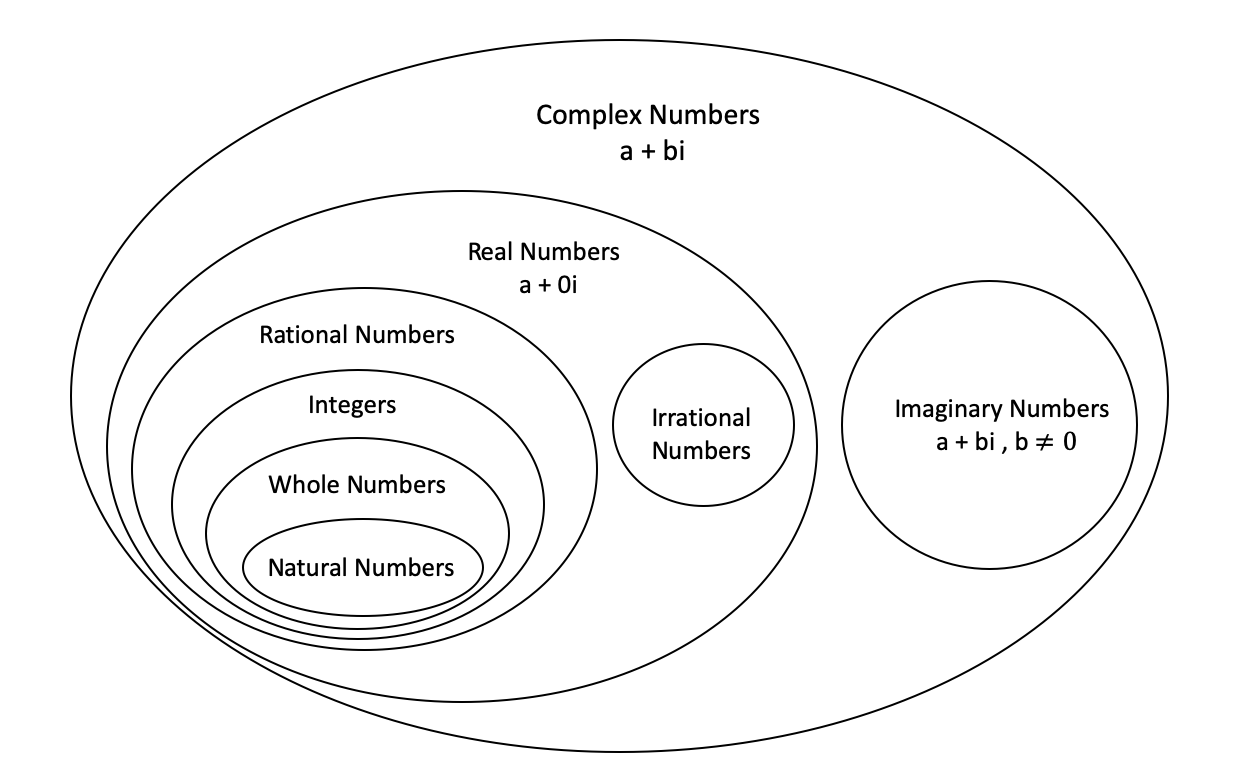
\includegraphics[width=1\linewidth]{figure/1-numbertypes} \end{center}

\hypertarget{complex-numbers}{%
\subsection{Complex numbers}\label{complex-numbers}}

\begin{itemize}
\tightlist
\item
  Every number in number system taken as a complex number
\item
  A number of the form \(a+ib\) is called a complex number when \(a\) and \(b\) are real numbers and \(i=\sqrt{-1}\).
\item
  We call `\(a\)' the real part and `\(b\)' the imaginary part of the complex number \(a+ib\).
\item
  IF \(a=0\) the number \(ib\) is said to be purely imaginary, if \(b=0\) the number \(a\) is real.
\item
  A pair of complex number \(a+ib\) and \(a-ib\) are said to be conjugate of each other.
\item
  Show that the sum and product of a complex number and its conjugate complex are both real.
\end{itemize}

Let \(x+iy\) be a complex number and \(x-iy\) its conjugate complex.

\[Sum = (x+iy)+(x-iy) = 2x\]\\
\[Product = (x+iy).(x-iy) = x^{2}+y^{2}\]

\begin{itemize}
\tightlist
\item
  Let \(a+ib\) and \(c+id\) be two complex numbers. Then
\end{itemize}

\textbf{Addition.} \((a+ib) + (c+id)= (a+c)+i(b+d)\)

\textbf{Subtraction} \((a+ib) - (c+id)= (a-c)+i(b-d)\)

\textbf{Multiplication} \((a+ib) \times (c+id)= ac-bd+i(ad+bc)\)

\textbf{Addition.} \(\frac{a+ib}{c+id}= \frac{a+ib}{c+id}.\frac{c-id}{c-id}= \frac{ac+bd}{c^2+d^2}+i\frac{bc-ad}{c^2+d^2}\)

\begin{itemize}
\tightlist
\item
  Complex numbers are denoted by \(\mathbb{C}\)
\end{itemize}

\hypertarget{imaginary-numbers}{%
\subsection{Imaginary numbers}\label{imaginary-numbers}}

\begin{itemize}
\tightlist
\item
  A number does not exist in the number line is called imaginary number.
\item
  For example square root of negative numbers are imaginary numbers. It is denoted by \(i\).
  i.e \[\sqrt{-1}=i\] \newline
  \[i^{2} = – 1\]
\item
  So there is no real number \(i\) that satisfies the above equation.
\item
  The quantity \(i\) is called the unit imaginary number.
\end{itemize}

\textbf{Geometrical Representation of imaginary numbers}

\begin{center}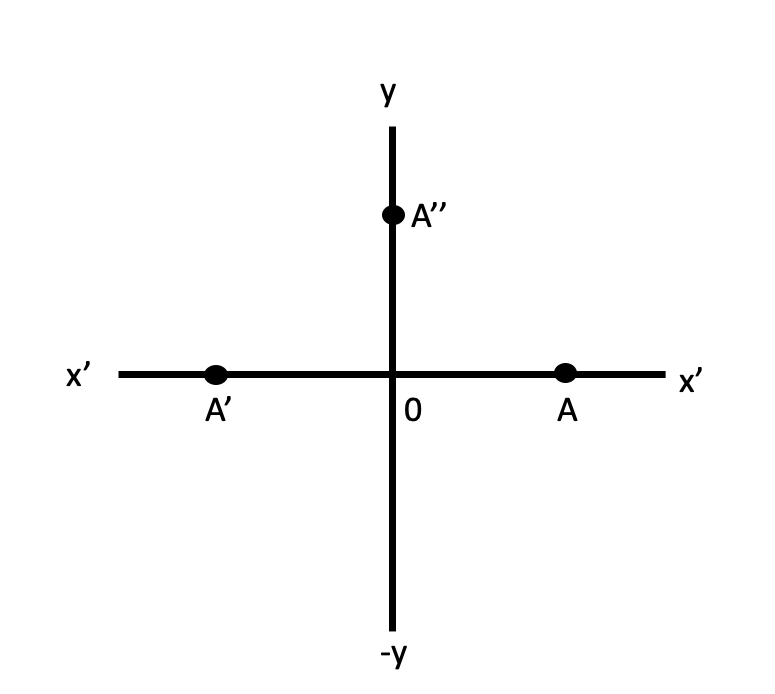
\includegraphics[width=0.5\linewidth]{figure/1-ImgNum} \end{center}

\begin{itemize}
\tightlist
\item
  Let OA be positive numbers which is represented by \(x\) and \(OA^\prime\) by \(-x\)
\item
  And \(-x= (i)^2x=i(ix)\) is on \(OX^{\prime}\)
\item
  It means that the multiplication of the real number \(x\) by \(i\) twice amounts to the rotation of OA through two right angles to reach \(OA^\prime\).
\item
  Thus, it means that multiplication of \(x\) by \(i\) is equivalent to the rotation of \(x\) through one right angle to reach \(OA^{\prime\prime}\).
\item
  Hence, y-axis is known as imaginary axis.
\item
  Multiplication by \(i\) rotates its direction through right angle.
\end{itemize}

\hypertarget{real-numbers}{%
\subsection{Real numbers}\label{real-numbers}}

\begin{itemize}
\tightlist
\item
  All numbers that can be represented on the number line are called real numbers.
\item
  The real numbers is the set of numbers containing all of the rational numbers and all of the irrational numbers.
\item
  The real numbers are ``all the numbers'' on the number line.
\item
  Real Numbers are denoted by \(\mathbb{R}\).
\end{itemize}

\hypertarget{rational-numbers}{%
\subsection{Rational numbers}\label{rational-numbers}}

\begin{itemize}
\item
  \(\mathbb{Q}\)
\item
  A rational number is defined as number of the form \(x/y\) where \(x\) and \(y\) are integers and \(y \neq 0\).
\item
  i.e Any number which can be expressed as in the form of \(p/q\) where \(p\) and \(q\) are the integers and \(q \neq 0\).
\item
  The set of rational numbers encloses the set of integers and fractions.
\item
  The rational numbers that are not integral will have decimal values. These values can be of two types

  \begin{itemize}
  \tightlist
  \item
    Terminating decimal fractions (finite decimal factors): For example \(1/5 = 0.5\) , \(13/5 = 2.6\).
  \item
    Non Terminating decimal fractions : The non terminating decimal fractions having two types.

    \begin{enumerate}
    \def\labelenumi{\roman{enumi})}
    \tightlist
    \item
      Non terminating periodic fractions
    \item
      Non terminating non periodic fractions
    \end{enumerate}
  \end{itemize}
\end{itemize}

\emph{i) Non terminating periodic fractions}

\begin{enumerate}
\def\labelenumi{\alph{enumi}.}
\item
  These are non terminating decimal fractions of the type \(a.b1b2b3b4b5 .....bmb1b2b3b4b5 .....bm\)
\item
  Examples

  \(19/6 = 3.16666666.....\)

  \(18/7 = 2.57142857142857.......\)

  \(21/9= 2.3333.......\)
\end{enumerate}

\emph{ii) Non terminating non periodic fractions}

\begin{enumerate}
\def\labelenumi{\alph{enumi}.}
\tightlist
\item
  These are non terminating and there is no periodic decimal places for that number.
\item
  i.e \(a.b1b2b3b4b5 .....bmc1c2.........\)
\item
  for example 6.789542587436512\ldots{}\ldots{}\ldots{}.
\end{enumerate}

\begin{itemize}
\tightlist
\item
  \textbf{So from above terminating and non terminating periodic fraction numbers belongs to rational numbers.}
\end{itemize}

\hypertarget{irrational-numbers}{%
\subsection{Irrational numbers}\label{irrational-numbers}}

\begin{itemize}
\tightlist
\item
  Irrational numbers are denoted by \(\mathbb{I}\)
\item
  An Irrational numbers are non terminating and non periodic fractions.
\item
  i.e irrational number is a number that cannot be written as a ratio \(x/y\) form (or fraction).
\item
  In decimal form, is never ends or repeats.
\item
  Examples for irrational numbers are \(\sqrt{2} = 1.414213......\), \(\pi = 3.14159265.......\), \(\sqrt{3}\), \(\sqrt{5}\) etc.
\end{itemize}

\hypertarget{integers}{%
\subsection{Integers}\label{integers}}

\begin{itemize}
\tightlist
\item
  All numbers that do not having the decimal places in them are called integers.
\item
  All whole numbers including Negative number + Positive number
\item
  \(\mathbb{Z} = \{...,-5,-4,-3,-2,-1,0,1,2,3,4,5,...\}\)
\item
  i.e the integer it may positive or negative or zero.
\item
  The set of integers generally written \(\mathbb{Z}\)for short.
\item
  Any integers are added, subtracted, or multiplied the result is always is an integer.
\item
  When any integers multiplied , each of the multiplied integer is called a factor or divisor of the resulting product
\end{itemize}

\hypertarget{whole-numbers}{%
\subsection{Whole numbers}\label{whole-numbers}}

\begin{itemize}
\tightlist
\item
  The set of whole numbers means narrator numbers and \(0\)
\item
  Whole numbers = \(\mathbb{W} = \{ 0,1,2,3,4,5,6,7,8,...\}\)
\end{itemize}

\hypertarget{natural-numbers}{%
\subsection{Natural numbers}\label{natural-numbers}}

\begin{itemize}
\tightlist
\item
  The counting numbers start with 1 and their end is not defined. Generally it is denoted by ``N''
\item
  i.e \(\mathbb{N} =\{1,2,3,4,...\}\)
\end{itemize}

\textbf{Reading :}

Dass, H. K. (2008). `Complex Numbers', \emph{Advanced Engineering Mathematics}. S. Chand Publishing. pp.~474-520.

\hypertarget{number-representations}{%
\section{Number representations}\label{number-representations}}

Decimal: The standard Hindu--Arabic numeral system using base ten.

Binary: The base-two numeral system used by computers.

Hexadecimal: Widely used by computer system designers and programmers, as they provide a more human-friendly representation of binary-coded values.

Octal: Occasionally used by computer system designers and programmers.

Duodecimal: The most convenient numeral system, due to twelve's divisibility by a wide range of the most elemental numbers \{1, 2, 3, 4\}.

Sexagesimal: Originated with the ancient Sumerians in the 3rd millennium BC, was passed down to the ancient Babylonians

(See positional notation for information on other bases)

Roman numerals: The numeral system of ancient Rome, still occasionally used today.

Tally marks: usually used for counting things that increase by small amounts and don't change very quickly.

Fractions: A representation of a non-integer as a ratio of two integers. These include improper fractions as well as mixed numbers.

Continued fraction: An expression obtained through an iterative process of representing a number as the sum of its integer part and the reciprocal of another number, then writing this other number as the sum of its integer part and another reciprocal, and so on.

Scientific notation: A method for writing very small and very large numbers using powers of 10. When used in science, such a number also conveys the precision of measurement using significant figures.

Knuth's up-arrow notation, Conway chained arrow notation, and Bowers's operators : Notations that allow the concise representation of some extremely large integers such as Graham's number.

\url{https://en.wikipedia.org/wiki/List_of_types_of_numbers}

\url{https://byjus.com/maths/number-system/}

\url{https://www.researchgate.net/publication/320677641_Number_System}

\url{http://www.compsci.hunter.cuny.edu/~sweiss/resources/BinaryNumbers.pdf}

\url{https://www.cs.bu.edu/courses/cs101a1/slides/CS101.Lect15.BinaryNumbers.ppt.pdf}

\url{https://www.eecs.wsu.edu/~ee314/handouts/numsys.pdf}

\url{http://www.uobabylon.edu.iq/eprints/publication_3_8400_6187.pdf}

\url{https://www.cs.princeton.edu/courses/archive/spr15/cos217/lectures/03_NumberSystems.pdf}

\href{https://www.ukessays.com/essays/social-work/number-system-is-used-in-it-applications-social-work-essay.php}{Number system is used in IT applications}

\begin{itemize}
\tightlist
\item
  Number Systems \href{https://www.topperlearning.com/ncert-solutions/cbse-class-9-mathematics/mathematics-ix/number-systems}{Rational, irrational numbers}
\end{itemize}

\hypertarget{sequences-and-series}{%
\chapter{Sequences and Series}\label{sequences-and-series}}

\hypertarget{sequences}{%
\section{Sequences}\label{sequences}}

\begin{itemize}
\tightlist
\item
  A \textbf{Sequence} can be thought of as a list of numbers written in a definite order:
  \[a_{1}, a_{2}, a_{3}, a_{4}, ..., a_{n}, ...\]
\item
  The number \(a_{1}\) is called the \emph{first term}, \(a_{2}\) is the \emph{second term}, and in general \(a_{n}\) is called the \(n^{th}\) \emph{term}.
\item
  We will deal exclusively with infinite sequences and so each term \(a_{n}\) will have a successor \(a_{n+1}\)
\item
  Notice that for every positive integer \(n\) there is a corresponding number \(a_{n}\) and so a sequence can be defined as a function whose domain is the set of positive integers.
\item
  But we usually write \(a_{n}\) instead of the function notation \(f(n)\) for the value of the function at the number \(n\).
\item
  \textbf{Notation:} The sequence \(\{a_{1}, a_{2}, a_{3},...\}\) is also denoted by
  \[\{a_{n}\}\] or \[\{a_{n}\}_{n=1}^{\infty}\]
\item
  Some sequences can be defined by giving a formula for the \(n\)th term.
\item
  In the following examples we give three descriptions of the sequences:

  \begin{enumerate}
  \def\labelenumi{\roman{enumi}.}
  \tightlist
  \item
    by using the preceding notation
  \item
    by using the defining formula
  \item
    by writing out the terms of the sequence
  \end{enumerate}
\item
  Notice that \(n\) doesn't have to start at 1.
\end{itemize}

\begin{enumerate}
\def\labelenumi{\alph{enumi})}
\item
  \(\{\frac{n}{n+1}\}_{n=1}^{\infty} \hspace{5em} a_{n} = \frac{n}{n+1}\hspace{5em}\{\frac{1}{2},\frac{2}{3}, \frac{3}{4}, \frac{4}{5},..., \frac{n}{n+1},... \}\)
\item
  \(\{\frac{(-1)^n(n+1)}{3^{n}}\}_{n=1}^{\infty} \hspace{5em} a_{n} = \frac{(-1)^n(n+1)}{3^{n}}\hspace{5em}\{-\frac{2}{3},\frac{3}{9}, -\frac{4}{27}, \frac{5}{81},..., \frac{(-1)^n(n+1)}{3^{n}},... \}\)
\item
  \(\{\sqrt{n-3}\}_{n=3}^{\infty} \hspace{5em} a_{n} = \sqrt{n-3}, n\geq3\hspace{5em}\{0,1,\sqrt{2}, \sqrt{3},..., \sqrt{n-3},...\}\)
\item
  \(\{cos\frac{n\pi}{6}\}_{n=0}^{\infty} \hspace{5em} a_{n} = cos\frac{n\pi}{6}, n\geq 0 \hspace{5em}\{1, \frac{\sqrt{3}}{2},\frac{1}{2}, 0,...,cos\frac{n\pi}{6},...\}\)
\end{enumerate}

\textbf{Example}

Find a formula for the general term \(a_{n}\) of the sequence
\[\{\frac{3}{5},-\frac{4}{25}, \frac{5}{125}, -\frac{6}{625}, \frac{7}{3125},...\}\]
assuming that the pattern of the first few terms continues.

\emph{SOLUTION}

We are given that

\hypertarget{series}{%
\section{Series}\label{series}}

Reading:

Stewart, J., Clegg, D. K., \& Watson, S. (2020). `Infinite Sequences and Series', \emph{Calculus: early transcendentals}. Cengage Learning.

\hypertarget{introduction-to-logic}{%
\chapter{Introduction to Logic}\label{introduction-to-logic}}

\hypertarget{boolean-algebra}{%
\chapter{Boolean Algebra}\label{boolean-algebra}}

\hypertarget{differentiation-and-integration}{%
\chapter{Differentiation and Integration}\label{differentiation-and-integration}}

\hypertarget{descriptive-statistics}{%
\chapter{Descriptive Statistics}\label{descriptive-statistics}}

\pagenumbering{arabic}

\hypertarget{introduction-to-statistics}{%
\section{Introduction to Statistics}\label{introduction-to-statistics}}

\hypertarget{some-basic-terminologies-used-in-statistics}{%
\subsection{Some Basic Terminologies Used in Statistics}\label{some-basic-terminologies-used-in-statistics}}

\textbf{i Population}

\begin{itemize}
\tightlist
\item
  The set of \textbf{all} possible elements in the universe of interest to the researcher
\end{itemize}

\textbf{ii Sample}

\begin{itemize}
\tightlist
\item
  A Sample is a \textbf{subset} (a portion or part) of the population of interest
\item
  The sample must be a representative of the population of interest
\end{itemize}

\textbf{iii Element}

\begin{itemize}
\tightlist
\item
  Element is an \textbf{entity or object} which the information is collected.
\item
  \emph{Eg: Student, household, farm, company, tomato plant}
\end{itemize}

\textbf{iv Variable}

\begin{itemize}
\tightlist
\item
  A variable is \textbf{a feature characteristic which has different `values' or categories for different elements} (items/subjects/individuals)
\item
  \emph{Eg: Gender of client, brand of mobile phones, risk level, number of emails received per day, age of client, income of client}
\end{itemize}

\textbf{v Data}

\begin{itemize}
\item
  Data are \textbf{measurements or facts} that are collected from a statistical unit/entity of interest
\item
  We collect data on variables
\item
  Data are raw numbers or facts that must be processed (analysed) to get useful information.
\item
  We get information from data.
\item
  \emph{Eg:}
\end{itemize}

\textbf{\emph{Variable:}} \emph{Age (in years) of client}

\textbf{\emph{Data:}} \emph{21, 45, 18, 32, 30, 22, 23, 27}

\textbf{\emph{Information:}}

\emph{The mean age is 27.25 years}

\emph{The minimum age is 18 years}

\emph{The range of ages is 18-45}

\emph{The percentage of clients below 25 years of age: 50\%}

\textbf{vi Statistic}

\begin{itemize}
\tightlist
\item
  \textbf{Characteristic} of a \textbf{sample}
\item
  The value which calculated based on sample data
\end{itemize}

\textbf{vii Parameter}

\begin{itemize}
\tightlist
\item
  \textbf{Characteristic} of a \textbf{population}
\item
  The value which calculated based on population data
\end{itemize}

\textbf{viii Census}

\begin{itemize}
\tightlist
\item
  When a researcher \textbf{gathers data from the whole population for a given measurement,} it is called a census
\end{itemize}

\textbf{ix Sampling}

\begin{itemize}
\tightlist
\item
  When a researcher \textbf{gathers data from a sample of the population for a given measurement,} it is called sampling
\item
  The process of selecting a sample is also called sampling
\end{itemize}

\textbf{Why take a sample instead of studying every member of the population ?}

\begin{itemize}
\tightlist
\item
  Prohibitive cost of census
\item
  Destruction of item being studied may be required
\item
  Not possible to test or inspect all members of a population being studied.
\end{itemize}

\hypertarget{branches-of-statistics}{%
\subsection{Branches of Statistics}\label{branches-of-statistics}}

\begin{figure}

{\centering 
\includegraphics[width=1\linewidth]{figure/box1-1} 

}

\end{figure}

\textbf{i Descriptive Statistics}

\begin{itemize}
\tightlist
\item
  Descriptive statistics consists of organizing, summarizing and presenting data in an informative way.
\item
  The main purpose of descriptive statistics is to provide an overview of the data collected.
\item
  Descriptive statistics describes the data collected through frequency tables, graphs and summary measures (mean, variance, quartiles, etc.).
\end{itemize}

\textbf{ii Inferential Statistics}

\begin{itemize}
\tightlist
\item
  In inferential statistics sample data are used to draw inferences (i.e.~derive conclusions) or make predictions about the populations from which the sample has been taken.
\item
  This includes methods used to make decisions, estimates, predictions or generalizations about a population based on a sample.
\item
  This includes point estimations, interval estimation, test of hypotheses, regression analysis, time series analysis, multivariate analysis, etc.
\end{itemize}

\hypertarget{types-of-variables}{%
\subsection{Types of Variables}\label{types-of-variables}}

\begin{figure}

{\centering 
\includegraphics[width=1\linewidth]{figure/box2-1} 

}

\end{figure}

\hypertarget{qualitative-quantitative-variables}{%
\subsubsection{Qualitative / Quantitative Variables}\label{qualitative-quantitative-variables}}

\textbf{i Qualitative variable (Categorical variable)}

\begin{itemize}
\tightlist
\item
  The characteristic is a quality.
\item
  The data are categories.
\item
  They cannot be given numerical values.
\item
  However, it may be given a numerical label
\item
  Qualitative variables are sometimes referred as categorical variables.
\item
  \emph{Eg:}
\end{itemize}

\emph{Gender:}

\emph{Age group:}

\emph{Education level:}

\emph{A/L stream:}

\emph{Degree type:}

\emph{Hair colour: }

\emph{FIT student batch:}

\emph{Undergraduate level:}

\emph{Grade that you can obtain for CM 1110/ CM1130}

\textbf{ii Quantitative variable }

\begin{itemize}
\tightlist
\item
  The characteristic is a quantity
\item
  The data are numbers
\item
  Quantitative data require numeric values that indicate how much or how many.
\item
  They are obtained by counting or measuring with some scale
\item
  \emph{Eg: }
\end{itemize}

\emph{Number of family members:}

\emph{Number of emails received per day:}

\emph{Weight of a student:}

\emph{Age:}

\emph{Credit balance in the SIM card:}

\emph{Time remaining in class:}

\emph{Temperature:}

\emph{Marks }

\hypertarget{discrete-continuous-variables}{%
\subsubsection{Discrete/ Continuous Variables}\label{discrete-continuous-variables}}

\begin{itemize}
\tightlist
\item
  Quantitative variables can be classified as either discrete or continuous.
\end{itemize}

\textbf{i Discrete Variables}

\begin{itemize}
\tightlist
\item
  Quantitative
\item
  Usually the data are obtained by counting
\item
  There are impossible values between any two possible values
\item
  \emph{Eg:}
\end{itemize}

\emph{Number of family members:}

\emph{Number of emails received per day:}

\textbf{ii Continuous Variables}

\begin{itemize}
\tightlist
\item
  Quantitative
\item
  Usually, the data are obtained by measuring with a scale
\item
  There are no impossible values between any two possible values.(any value between any two possible values is also a possible value)
\item
  i.e a continuous variable can take any value within a specified range.
\item
  \emph{Eg:}
\end{itemize}

\emph{Weight of a student:}

\emph{Age:}

\emph{Credit balance in the SIM card:}

\emph{Time remaining in class:}

\emph{Temperature:}

\emph{Marks}

\hypertarget{scales-of-measurements}{%
\subsection{Scales of Measurements}\label{scales-of-measurements}}

\begin{figure}

{\centering 
\includegraphics[width=1\linewidth]{figure/box3-1} 

}

\end{figure}

\begin{itemize}
\tightlist
\item
  There are four levels of measurements called, \textbf{nominal, ordinal, interval and ratio.}
\item
  Each levels has its own rules and restrictions
\item
  Different levels of measurement contains different amount of information with respect to whatever the data are measuring
\end{itemize}

\textbf{i Nominal Scale}

\begin{itemize}
\tightlist
\item
  Qualitative
\item
  No order or ranking in categories.
\item
  These categories have to be mutually exclusive, i.e.~it should not be possible to place an individual or object in more than one category
\item
  A name of a category can be substituted by a number, but it will be mere label and have no numerical meaning
\end{itemize}

\textbf{ii Ordinal Scale}

\begin{itemize}
\tightlist
\item
  Qualitative
\item
  Categories can be ordered or ranked
\item
  A name of a category can be substituted by a number, but such a sequence does not indicate absolute quantities.
\item
  Difference between any two numbers on the scale does not have a numerical meaningful.
\item
  It cannot be assumed that the differences between adjacent numbers on the scale are equal.
\end{itemize}

\textbf{iii Interval Scale}

\begin{itemize}
\tightlist
\item
  Quantitative
\item
  Data can be ordered or ranked
\item
  There is no absolute zero point. Zero is only an arbitrary point with which other values can compare
\item
  Difference between two numbers is a meaningful numerical value
\item
  Ration of two numbers is not a meaningful numerical value.
\end{itemize}

\textbf{iv Ratio Scale}

\begin{itemize}
\tightlist
\item
  Quantitative
\item
  Highest level of measurement
\item
  There exist an absolute zero point (It has a true zero point)
\item
  Ratio between different measurements is meaningful
\end{itemize}

\newpage

\hypertarget{presentation-of-data}{%
\section{Presentation of Data}\label{presentation-of-data}}

The sinking of the Titanic is one of the most infamous shipwrecks in history.

On April 15, 1912, during her maiden voyage, the widely considered ``unsinkable'' RMS Titanic sank after colliding with an iceberg. Unfortunately, there weren't enough lifeboats for everyone onboard, resulting in the death of 1502 out of 2224 passengers and crew

\footnote{Data source: \url{https://www.kaggle.com/varimp/a-mostly-tidyverse-tour-of-the-titanic}}

Here's a quick summary of our variables:

\begin{longtable}[]{@{}ll@{}}
\toprule
\begin{minipage}[b]{0.49\columnwidth}\raggedright
Variable Name\strut
\end{minipage} & \begin{minipage}[b]{0.45\columnwidth}\raggedright
Description\strut
\end{minipage}\tabularnewline
\midrule
\endhead
\begin{minipage}[t]{0.49\columnwidth}\raggedright
PassengerID\strut
\end{minipage} & \begin{minipage}[t]{0.45\columnwidth}\raggedright
Passenger ID (just a row number, so obviously not useful for prediction)\strut
\end{minipage}\tabularnewline
\begin{minipage}[t]{0.49\columnwidth}\raggedright
Survived\strut
\end{minipage} & \begin{minipage}[t]{0.45\columnwidth}\raggedright
Survived (1) or died (0)\strut
\end{minipage}\tabularnewline
\begin{minipage}[t]{0.49\columnwidth}\raggedright
Pclass\strut
\end{minipage} & \begin{minipage}[t]{0.45\columnwidth}\raggedright
Passenger class (first, second or third)\strut
\end{minipage}\tabularnewline
\begin{minipage}[t]{0.49\columnwidth}\raggedright
Name\strut
\end{minipage} & \begin{minipage}[t]{0.45\columnwidth}\raggedright
Passenger name\strut
\end{minipage}\tabularnewline
\begin{minipage}[t]{0.49\columnwidth}\raggedright
Gender\strut
\end{minipage} & \begin{minipage}[t]{0.45\columnwidth}\raggedright
Passenger Gender\strut
\end{minipage}\tabularnewline
\begin{minipage}[t]{0.49\columnwidth}\raggedright
Age\strut
\end{minipage} & \begin{minipage}[t]{0.45\columnwidth}\raggedright
Passenger age\strut
\end{minipage}\tabularnewline
\begin{minipage}[t]{0.49\columnwidth}\raggedright
SibSp\strut
\end{minipage} & \begin{minipage}[t]{0.45\columnwidth}\raggedright
Number of siblings/spouses aboard\strut
\end{minipage}\tabularnewline
\begin{minipage}[t]{0.49\columnwidth}\raggedright
Parch\strut
\end{minipage} & \begin{minipage}[t]{0.45\columnwidth}\raggedright
Number of parents/children aboard\strut
\end{minipage}\tabularnewline
\begin{minipage}[t]{0.49\columnwidth}\raggedright
Ticket\strut
\end{minipage} & \begin{minipage}[t]{0.45\columnwidth}\raggedright
Ticket number\strut
\end{minipage}\tabularnewline
\begin{minipage}[t]{0.49\columnwidth}\raggedright
Fare\strut
\end{minipage} & \begin{minipage}[t]{0.45\columnwidth}\raggedright
Fare\strut
\end{minipage}\tabularnewline
\begin{minipage}[t]{0.49\columnwidth}\raggedright
Cabin\strut
\end{minipage} & \begin{minipage}[t]{0.45\columnwidth}\raggedright
Cabin\strut
\end{minipage}\tabularnewline
\begin{minipage}[t]{0.49\columnwidth}\raggedright
Embarked\strut
\end{minipage} & \begin{minipage}[t]{0.45\columnwidth}\raggedright
Port of embarkation (S = Southampton, C = Cherbourg, Q = Queenstown)\strut
\end{minipage}\tabularnewline
\bottomrule
\end{longtable}

\hypertarget{tabular-presentations-of-data}{%
\subsection{Tabular Presentations of Data}\label{tabular-presentations-of-data}}

\textbf{Raw Data}

\begin{itemize}
\tightlist
\item
  Raw data are collected data that have not been organized numerically
\item
  Eg: Passenger age
\end{itemize}

\begin{verbatim}
##   PassengerId Survived Pclass
## 1           1        0      3
## 2           2        1      1
## 3           3        1      3
## 4           4        1      1
## 5           5        0      3
## 6           6        0      3
##                                                  Name    Sex Age SibSp Parch
## 1                             Braund, Mr. Owen Harris   male  22     1     0
## 2 Cumings, Mrs. John Bradley (Florence Briggs Thayer) female  38     1     0
## 3                              Heikkinen, Miss. Laina female  26     0     0
## 4        Futrelle, Mrs. Jacques Heath (Lily May Peel) female  35     1     0
## 5                            Allen, Mr. William Henry   male  35     0     0
## 6                                    Moran, Mr. James   male  NA     0     0
##             Ticket    Fare Cabin Embarked
## 1        A/5 21171  7.2500              S
## 2         PC 17599 71.2833   C85        C
## 3 STON/O2. 3101282  7.9250              S
## 4           113803 53.1000  C123        S
## 5           373450  8.0500              S
## 6           330877  8.4583              Q
\end{verbatim}

\begin{verbatim}
##  [1] 22 38 26 35 35 NA 54  2 27 14  4 58 20 39 14 55  2 NA 31 NA 35 34 15 28  8
## [26] 38 NA 19 NA NA 40 NA NA 66 28 42 NA 21 18 14
\end{verbatim}

\textbf{An array}

\begin{itemize}
\tightlist
\item
  An array is an arrangement of raw numerical data in ascending or descending order of magnitude.
\item
  Eg: Passenger age
\end{itemize}

\begin{verbatim}
##  [1]  2  2  4  8 14 14 14 15 18 19 20 21 22 26 27 28 28 31 34 35 35 35 38 38 39
## [26] 40 42 54 55 58 66
\end{verbatim}

\textbf{Frequency Table (Frequency Distributions)}

\begin{itemize}
\tightlist
\item
  A frequency table (frequency distribution) is a listing of the values a variable takes in a data set, along with how often (frequently) each value occurs
\item
  frequency can be recorded as a

  \begin{itemize}
  \tightlist
  \item
    \textbf{frequency or count:} the number of times a value occurs, or
  \item
    \textbf{percentage frequency:} the percentage of times a value occurs
  \end{itemize}
\item
  Percentage frequency can be calculated as,
\end{itemize}

\[Percentage frequency = \frac{a}{b} \times100 \%\]

\begin{itemize}
\tightlist
\item
  The objective of constructing a frequency table are as follows

  \begin{itemize}
  \tightlist
  \item
    to organize the data in a meaningful manner
  \item
    to determine the nature or shape of the distribution
  \item
    to draw charts and graphs for the presentation of data
  \item
    to facilitate computational procedures for measures of average and spread
  \item
    to make comparisons between different data sets
  \end{itemize}
\item
  There are two basic types of frequency tables

  \begin{enumerate}
  \def\labelenumi{\arabic{enumi}.}
  \tightlist
  \item
    Simple frequency tables (Ungrouped frequency distribution)
  \item
    Grouped frequency distribution
  \end{enumerate}
\end{itemize}

\hypertarget{simple-frequency-table-ungrouped-frequency-distribution}{%
\subsubsection{Simple frequency table (Ungrouped frequency distribution)}\label{simple-frequency-table-ungrouped-frequency-distribution}}

\begin{itemize}
\tightlist
\item
  Each possible value or category is taken as a class
\item
  More suitable for

  \begin{itemize}
  \tightlist
  \item
    Qualitative variables
  \item
    Discrete variables
  \end{itemize}
\item
  Sometimes construct for continuous variables when there is a small number of possible values between the minimum and maximum.
\end{itemize}

Examples:

\textbf{CASE I:}

Example 1

The native countries of 56 students from a certain education institute are as follows:

\begin{verbatim}
##  [1] "SL" "BD" "SL" "SL" "SL" "SL" "IN" "SL" "SL" "SL" "BD" "SL" "SL" "SL" "IN"
## [16] "SL" "SL" "BD" "SL" "SL" "SL" "SL" "SL" "SL" "SL" "SL" "SL" "MD" "SL" "SL"
## [31] "SL" "SL" "SL" "SL" "PK" "MD" "PK" "SL" "SL" "SL" "SL" "SL" "PK" "MD" "SL"
## [46] "SL" "SL" "SL" "SL" "SL" "SL" "SL" "SL" "SL" "MD" "MD"
\end{verbatim}

BD- Bangladesh, IN-India, MD-Maldives, PK-Pakistan, SL- Sri Lanka

Construct a frequency table

\begin{verbatim}
##  Native Country Count Percentage (%)
##      Bangladesh     3          5.357
##           India     2          3.571
##        Maldives     5          8.929
##        Pakistan     3          5.357
##       Sri Lanka    43         76.786
##           Total    56        100.000
\end{verbatim}

\textbf{CASE II:}

Example 2

The grades of 30 students for Statistics are as follows:

\begin{verbatim}
##  [1] "B" "C" "B" "D" "B" "C" "C" "A" "B" "C" "C" "B" "E" "B" "B" "D" "D" "F" "B"
## [20] "D" "D" "A" "B" "A" "B" "C" "E" "A" "A"
\end{verbatim}

Construct a frequency table

\begin{verbatim}
##  Grade Count Percentage (%)
##      A     5         17.241
##      B    10         34.483
##      C     6         20.690
##      D     5         17.241
##      E     2          6.897
##      F     1          3.448
##  Total    29        100.000
\end{verbatim}

\textbf{CASE III:}

Example 3

The number of family members of a sample of undergraduates of Batch 19 are as follows:

\begin{verbatim}
##  [1] 7 5 3 4 5 4 3 6 4 4 5 2 7 4 5 6 4 4 3 5
\end{verbatim}

Construct a frequency table

\begin{verbatim}
##  Number of family members Count Percentage (%)
##                         2     1              5
##                         3     3             15
##                         4     7             35
##                         5     5             25
##                         6     2             10
##                         7     2             10
##                     Total    20            100
\end{verbatim}

\textbf{CASE IV:}

Example 4

The ages (in years) of a sample of undergraduates of Batch 19 are as follows:

\begin{verbatim}
##  [1] 21 22 22 23 22 24 24 23 21 22 23 22 22 23 21 21 22 23 22 23
\end{verbatim}

Construct a frequency table

\begin{verbatim}
##  Age (years) Count Percentage (%)
##           21     4             20
##           22     8             40
##           23     6             30
##           24     2             10
##        Total    20            100
\end{verbatim}

\hypertarget{grouped-frequency-distribution}{%
\subsubsection{Grouped frequency distribution}\label{grouped-frequency-distribution}}

\begin{itemize}
\tightlist
\item
  A grouped frequency distribution (table) is obtained by constructing classes (or intervals) for the data and then listing the corresponding number of values in each interval.
\item
  Suitable for quantitative variables with large number of possible values in the range of data.
\item
  Note that when items have been grouped in this way, their individual values are lost.
\item
  When studying about frequency distributions it is very important to know the meaning of the following terms
\end{itemize}

\textbf{i Class intervals}

\begin{itemize}
\tightlist
\item
  In a frequency distribution the total range of the observations are divided into a number of classes. Those are called \emph{class intervals}
\item
  Eg: Class intervals: 10-14, 15-19, 20-24, \ldots{}, 40-44
\end{itemize}

\textbf{ii Class limits}

\begin{itemize}
\tightlist
\item
  Class limits are the smallest and largest piece of data value that can fall into a given class.
\item
  In the class interval 10-14, the end numbers, 10 and 14, are called class limits
\item
  The smaller number (10) is the \emph{lower class limit}
\item
  The larger number (14) is the \emph{upper class limit}
\end{itemize}

\textbf{iii Class boundaries}

\begin{itemize}
\tightlist
\item
  Class boundaries are obtained by adding the upper limit of one class interval to the lower limit of the next-higher class interval and dividing by 2.
\item
  Class boundaries are also called \textbf{True class limits}
\item
  Class boundaries \textbf{should not} \emph{coincide with actual observations}
\end{itemize}

\begin{longtable}[]{@{}ll@{}}
\toprule
Class interval & Class boundaries\tabularnewline
\midrule
\endhead
10 - 14 & 9.5 -- 14.5\tabularnewline
15 - 19 & 14.5 -- 19.5\tabularnewline
20 - 24 & 19.5 -- 24.5\tabularnewline
25 - 29 & 24.5 -- 29.5\tabularnewline
30 - 34 & 29.5 -- 34.5\tabularnewline
35 - 39 & 34.5 -- 39.5\tabularnewline
40 - 44 & 39.5 -- 44.5\tabularnewline
\bottomrule
\end{longtable}

\textbf{iv The size or width of a class interval}

\begin{itemize}
\tightlist
\item
  The size or width of a class interval is the difference between the \emph{lower and upper class boundaries}
\item
  It is also referred to as the \emph{class width, class size, or class length}
\item
  Eg: The class width for the class 10-14 is = 14.5-9.5 = 5
\end{itemize}

\textbf{v The class mark ( Midpoint of the class)}

\begin{itemize}
\tightlist
\item
  Midpoint of the class
\item
  Also called as \emph{class midpoint}
\item
  \(\text{Midpoint of the class} = \frac{\text{Lower limit} + \text{Upper limit}}{2}\)
\end{itemize}

or

\begin{itemize}
\tightlist
\item
  \(\text{Midpoint of the class} = \frac{\text{Lower boundary} + \text{Upper boundary}}{2}\)
\end{itemize}

\textbf{vi Open class intervals}

\begin{itemize}
\item
  A class interval that, at least theoretically, has either no upper class limit or no lower class limit indicated is called an \emph{open class interval}
\item
  For example, referring to age groups of individuals, the class interval ``65 year and over'' is an open class interval
\end{itemize}

\textbf{Rules and Practices for constructing grouped frequency tables}

\begin{itemize}
\tightlist
\item
  Every data value should be in an interval
\item
  The intervals should be mutually exclusive
\item
  The classes of the distribution must be arrayed in size order.
\item
  The number of classes not less than 5 or not greater than 15 is recommended.
\item
  The following formula is often used to determine the number of classes:
  If n is the number of observations, then
\end{itemize}

\[\text{Number of classes} = \sqrt{n}\]

\[\text{Width of the class interval} = \frac{Range}{\sqrt{n}}= \frac{Min-Max}{\sqrt{n}}\]

\begin{itemize}
\tightlist
\item
  Data should be represented within classes having limits which the data can attain
\item
  Classes should be continuous
\item
  By convention, the beginning of the interval is given the appropriate exact value, rather than the end.\\
  Eg: intervals of 0-49, 50-99,100-149 would be preferred over the intervals 1-50, 51-100, 101-150 etc.
\item
  The number f observations falling into each category or class interval (class frequency) can be easily found using \emph{tally marks}.
\end{itemize}

Examples:

In a grouped frequency distribution, class intervals can be constructed in different ways

Example 1

\begin{longtable}[]{@{}ll@{}}
\toprule
Class interval & Number of students\tabularnewline
\midrule
\endhead
10 - 14 & 4\tabularnewline
15 - 19 & 5\tabularnewline
20 - 24 & 11\tabularnewline
25 - 29 & 9\tabularnewline
30 - 34 & 6\tabularnewline
35 - 39 & 3\tabularnewline
40 - 44 & 2\tabularnewline
\bottomrule
\end{longtable}

Example 2

\begin{longtable}[]{@{}ll@{}}
\toprule
Salary & Number of employees\tabularnewline
\midrule
\endhead
0 -- 1999 & 1\tabularnewline
2000 -- 3999 & 31\tabularnewline
4000 -- 5999 & 18\tabularnewline
6000 -- 7999 & 4\tabularnewline
8000 -- 9999 & 2\tabularnewline
10000 - 11999 & 1\tabularnewline
12000 -- 13999 & 0\tabularnewline
14000 -- 15999 & 0\tabularnewline
16000 -- 17999 & 1\tabularnewline
18000 -19999 & 1\tabularnewline
20000-21999 & 1\tabularnewline
\bottomrule
\end{longtable}

\begin{longtable}[]{@{}ll@{}}
\toprule
Salary & Number of employees\tabularnewline
\midrule
\endhead
0 -- 1999 & 1\tabularnewline
2000 -- 3999 & 31\tabularnewline
4000 -- 5999 & 18\tabularnewline
6000 -- 7999 & 4\tabularnewline
8000 -- 9999 & 2\tabularnewline
10000 - 15999 & 1\tabularnewline
16000 -- 21999 & 3\tabularnewline
Total & 60\tabularnewline
\bottomrule
\end{longtable}

\textbf{Example 3}

\begin{longtable}[]{@{}ll@{}}
\toprule
Salary & Number of employees\tabularnewline
\midrule
\endhead
Less than 2000 & 1\tabularnewline
2000 -- 2999 & 11\tabularnewline
3000 -- 3999 & 20\tabularnewline
4000 -- 5999 & 18\tabularnewline
6000 -- 9999 & 6\tabularnewline
Greater than or equal to 10000 & 4\tabularnewline
Total & 60\tabularnewline
\bottomrule
\end{longtable}

\hypertarget{two-way-frequency-table}{%
\subsubsection{Two-way frequency table}\label{two-way-frequency-table}}

\begin{itemize}
\tightlist
\item
  Cross tabulation, Cross classification table, Contingency table, Two-way table
\item
  Display the relationship between two or more qualitative variables (categorical variables (nominal or ordinal))
\end{itemize}

\begin{verbatim}
## # A tibble: 2 x 4
##   Survived First Second Third
##   <chr>    <dbl>  <dbl> <dbl>
## 1 died        80     97   372
## 2 Survived   136     87   119
\end{verbatim}

\begin{verbatim}
## # A tibble: 2 x 4
##   Survived First Second Third
##   <chr>    <dbl>  <dbl> <dbl>
## 1 died      0.37   0.53  0.76
## 2 Survived  0.63   0.47  0.24
\end{verbatim}

\hypertarget{graphic-presentations-of-data}{%
\subsection{Graphic Presentations of Data}\label{graphic-presentations-of-data}}

\begin{itemize}
\tightlist
\item
  A diagram is a visual form for presentation of statistical data.
\item
  The form of the diagram varies according to the nature of the data
\end{itemize}

\hypertarget{describing-qualitative-data}{%
\subsubsection{Describing Qualitative Data}\label{describing-qualitative-data}}

\begin{itemize}
\tightlist
\item
  Bar chart / Pie chart
\item
  Suitable for

  \begin{itemize}
  \tightlist
  \item
    Qualitative variables (nominal or ordinal)
  \item
    Discrete variables (when the number of bars or number of different values is small)
  \end{itemize}
\end{itemize}

\textbf{I Bar Chart}

\begin{itemize}
\tightlist
\item
  A bar graph uses bars to represent discrete categories of data
\item
  It can be drawn either on horizontal (more common) or vertical base
\item
  A rectangle of equal width is drawn for each category
\item
  The height (in vertical bar chart) or the length (in horizontal bar chart) of the rectangle is equal to the category's \textbf{frequency} or \textbf{percentage}.
\end{itemize}

\begin{center}
\includegraphics[width=1\linewidth]{figure/box6-1} \end{center}

\textbf{i Simple Bar Chart}

\begin{itemize}
\tightlist
\item
  Only one categorical variable can be presented
\item
  Often used in conjunction with simple frequency tables
\item
  The bars do not touch each other
\item
  The gaps between adjacent bars are same in length
\end{itemize}

\begin{tabular}{l|r|r}
\hline
Passenger class & Count & Percentage\\
\hline
First & 216 & 24.242\\
\hline
Second & 184 & 20.651\\
\hline
Third & 491 & 55.107\\
\hline
\end{tabular}

\begin{center}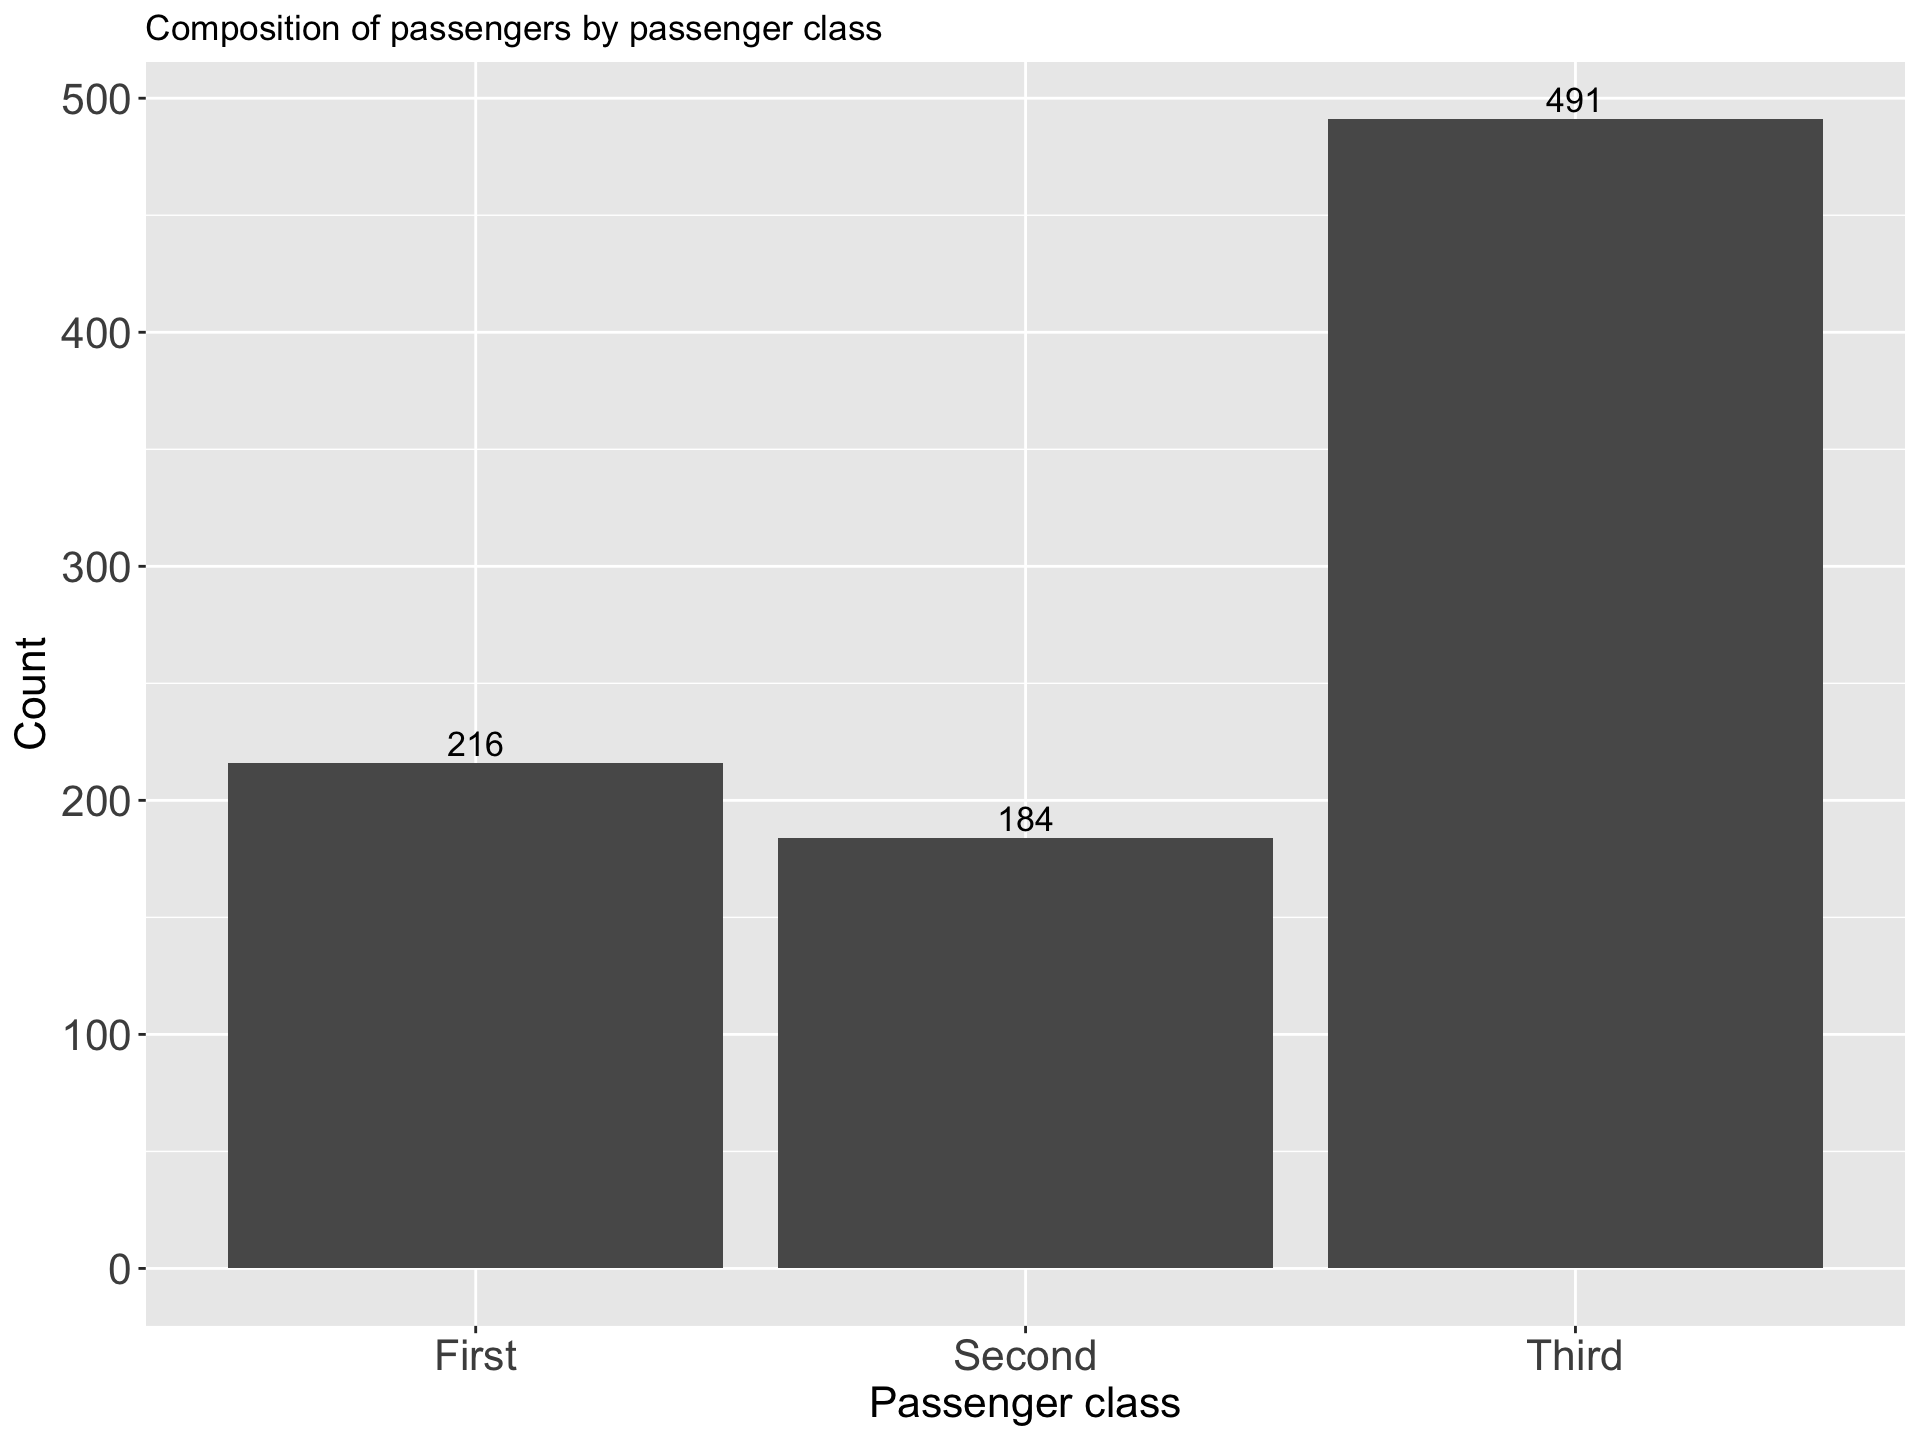
\includegraphics[width=0.8\linewidth]{figure/box8-1} \end{center}

\begin{center}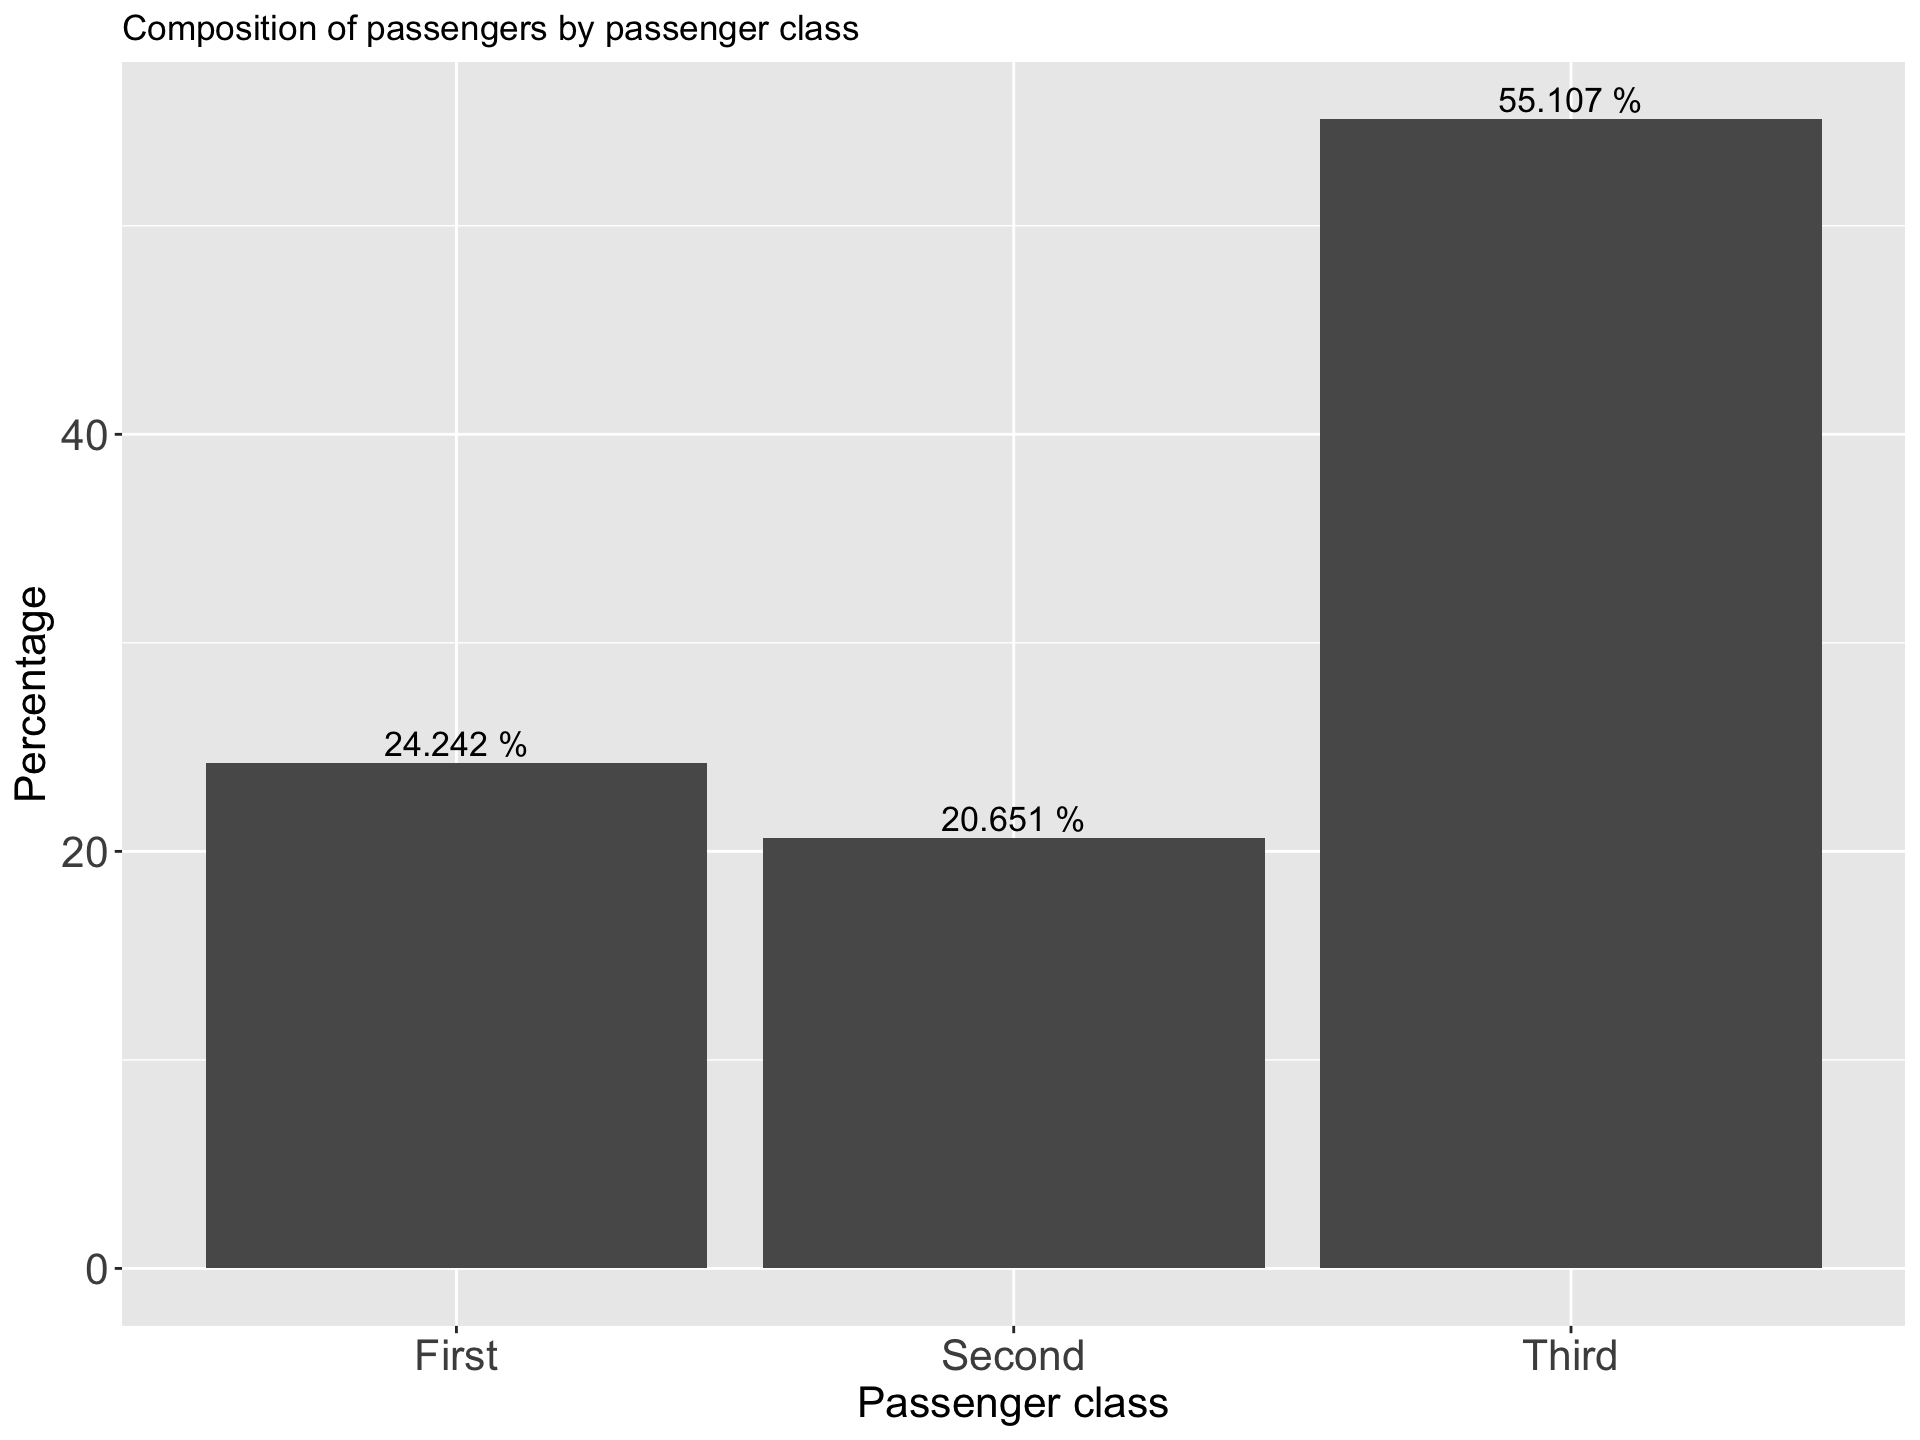
\includegraphics[width=0.8\linewidth]{figure/box9-1} \end{center}

\textbf{ii Component Bar Chart }

\begin{itemize}
\tightlist
\item
  \textbf{Sub divided bar chart/ Stacked bar chart}
\item
  Use to compare two or more qualitative variables (nominal or ordinal)
\item
  Often used in conjunction with two way tables
\item
  Start by drawing a simple bar chart with the total figures.
\item
  The bars are then divided into the component parts
\item
  Can be drawn on absolute figures or percentages
\item
  The various components should be kept in the same order in each bar
\item
  To distinguish different components from one another, different colours or shades can be used
\end{itemize}

\begin{tabular}{l|r|r|r}
\hline
Survived & First & Second & Third\\
\hline
died & 80 & 97 & 372\\
\hline
Survived & 136 & 87 & 119\\
\hline
\end{tabular}

\begin{center}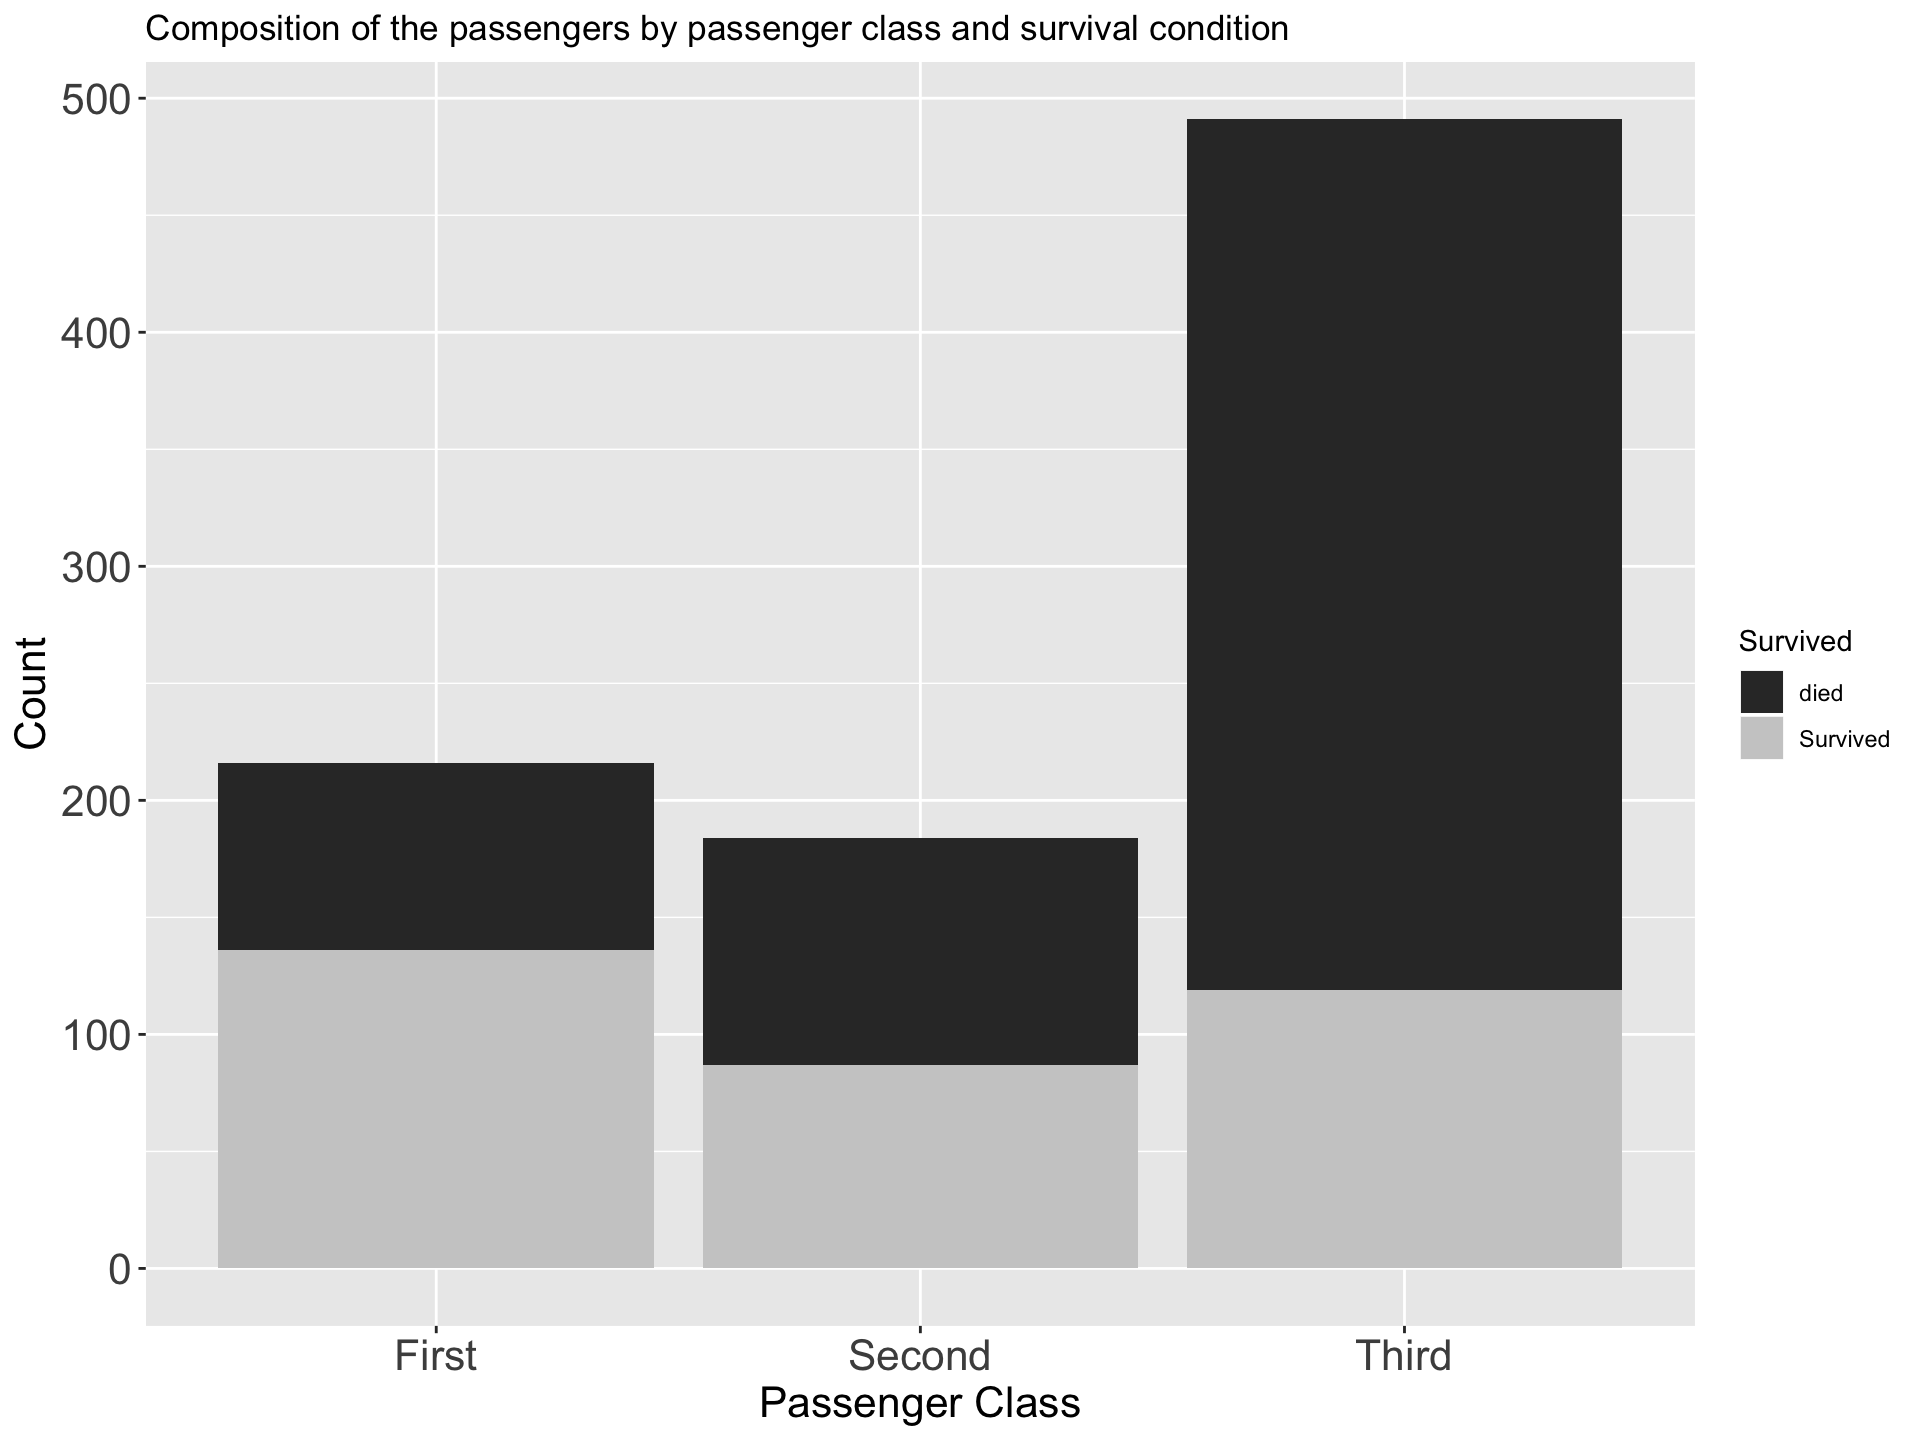
\includegraphics[width=0.8\linewidth]{figure/box10-1} \end{center}

\textbf{Percentage component bar chart}

\begin{itemize}
\tightlist
\item
  When sub-divided bar chart is drawn on percentage basis it is called percentage bar chart
\item
  The various components are expressed as percentage to the total
\item
  All bars are equal in height
\end{itemize}

\begin{tabular}{l|r|r|r}
\hline
Survived & First & Second & Third\\
\hline
died & 0.3703704 & 0.5271739 & 0.7576375\\
\hline
Survived & 0.6296296 & 0.4728261 & 0.2423625\\
\hline
\end{tabular}

\begin{center}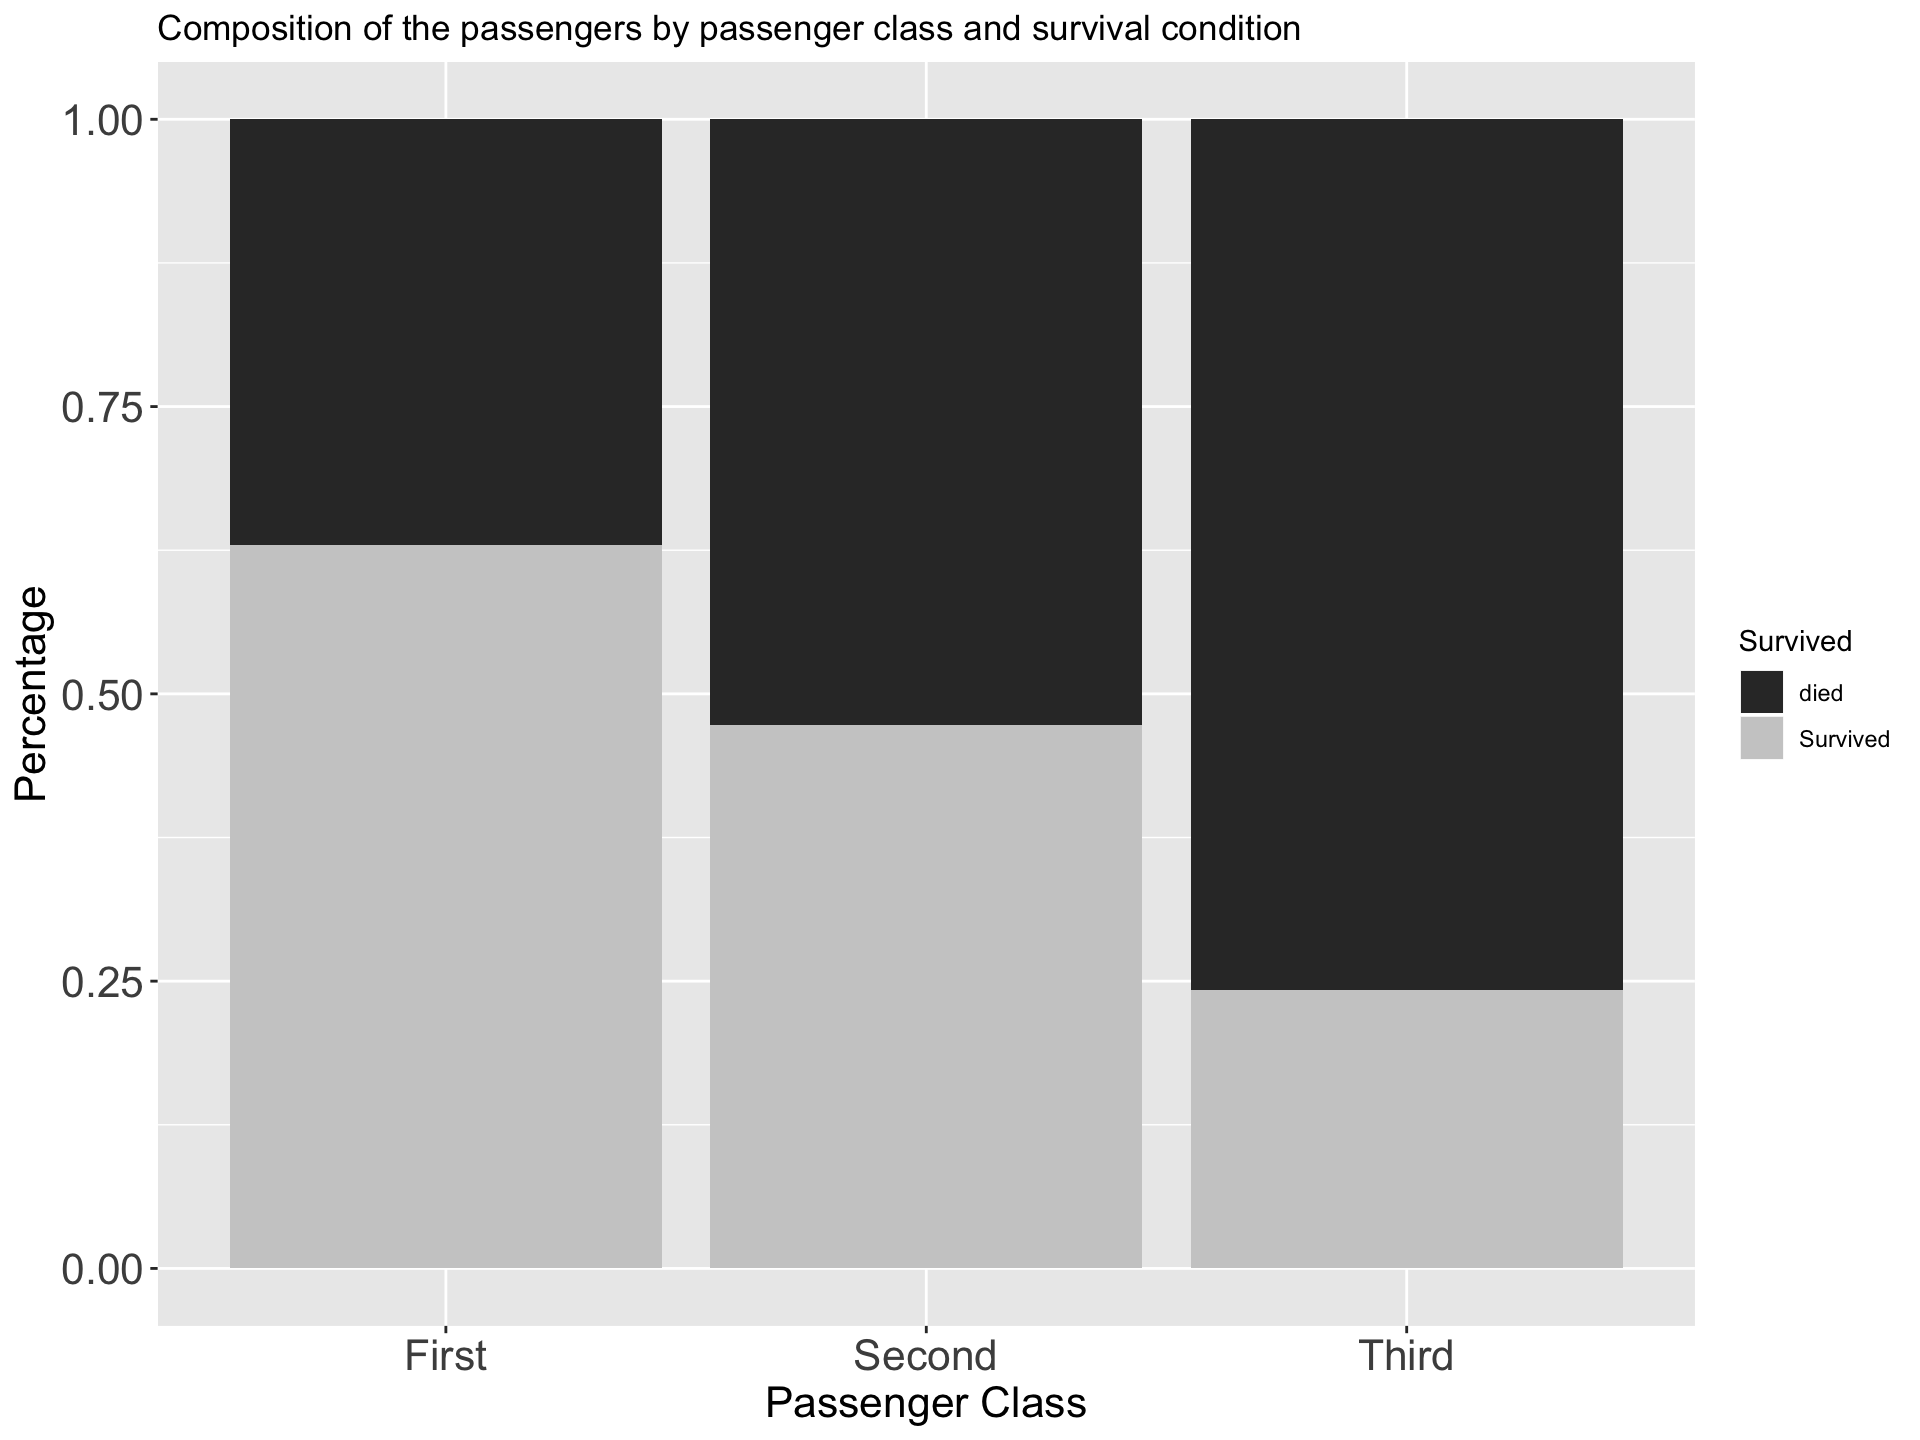
\includegraphics[width=0.8\linewidth]{figure/box11-1} \end{center}

\textbf{iii Multiple Bar Chart}

\begin{itemize}
\tightlist
\item
  Compound bar chart/ Cluster bar chart
\item
  Use to compare two or more qualitative variables (nominal or ordinal)
\item
  Often used in conjunction with two way tables
\item
  These bar charts are drawn side by side
\end{itemize}

\begin{tabular}{l|r|r|r}
\hline
Survived & First & Second & Third\\
\hline
died & 37.04 & 52.72 & 75.76\\
\hline
Survived & 62.96 & 47.28 & 24.24\\
\hline
\end{tabular}

\begin{center}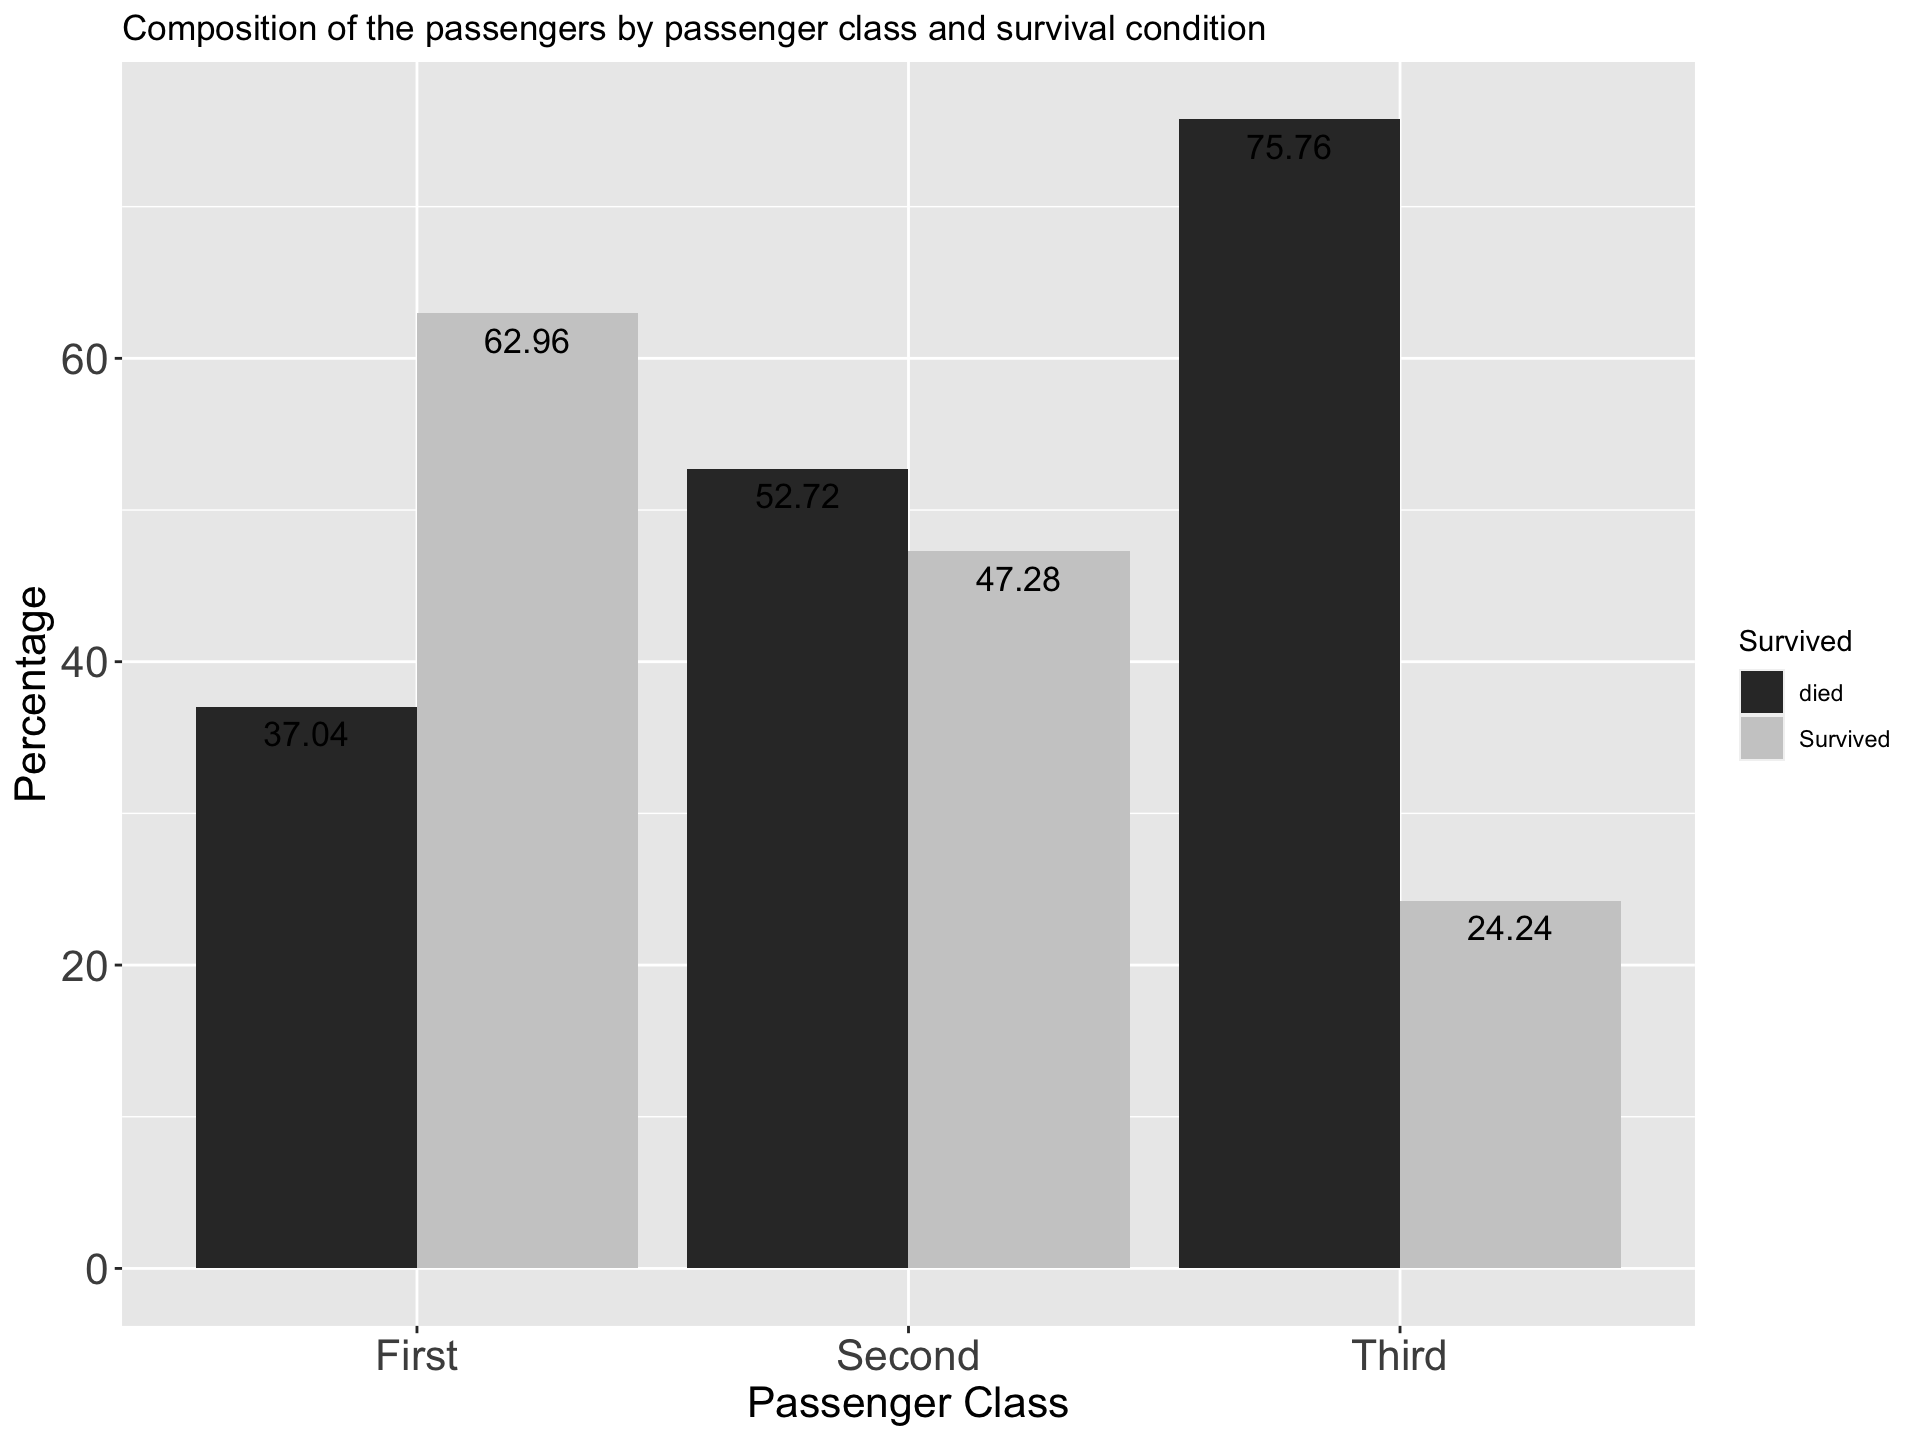
\includegraphics[width=0.8\linewidth]{figure/box12-1} \end{center}

\hypertarget{describing-quantitative-data}{%
\subsubsection{Describing Quantitative Data}\label{describing-quantitative-data}}

\begin{itemize}
\tightlist
\item
  Histogram/ Dot plot / Box plot/ Scatter plot
\end{itemize}

\textbf{II Histogram}

\begin{itemize}
\tightlist
\item
  Histogram looks similar to bar chart since it also has bars.
\item
  However, it is different from a bar chart in a number of aspects.
\item
  One main difference is that in the histogram, the bars are drawn attached to each other; there are no gaps between bars like in a bar chart.
\item
  Histogram is used to show the shape of the distribution of a \textbf{continuous variable}.
\item
  However, the histogram is also used for discrete variables when the data are grouped in to class intervals.
\item
  In a histogram, \textbf{the area of a bar should be proportional to the frequency of the corresponding class.}
\item
  If all the bars have the same width, then the height of a bar can represent the frequency.
\item
  The bar corresponding to a class interval should be drawn from the lower class boundary to the upper class boundary. In this way there will be no gaps between the bars.
\end{itemize}

Example: The marks(out of 50) of a group of students are recorded in the accompanying table. Draw a histogram for the data

\begin{longtable}[]{@{}ll@{}}
\toprule
Marks & Number of students\tabularnewline
\midrule
\endhead
10 - 14 & 4\tabularnewline
15 - 19 & 5\tabularnewline
20 - 24 & 11\tabularnewline
25 - 29 & 9\tabularnewline
30 - 34 & 6\tabularnewline
35 - 39 & 3\tabularnewline
40 - 44 & 2\tabularnewline
Total & 40\tabularnewline
\bottomrule
\end{longtable}

\begin{center}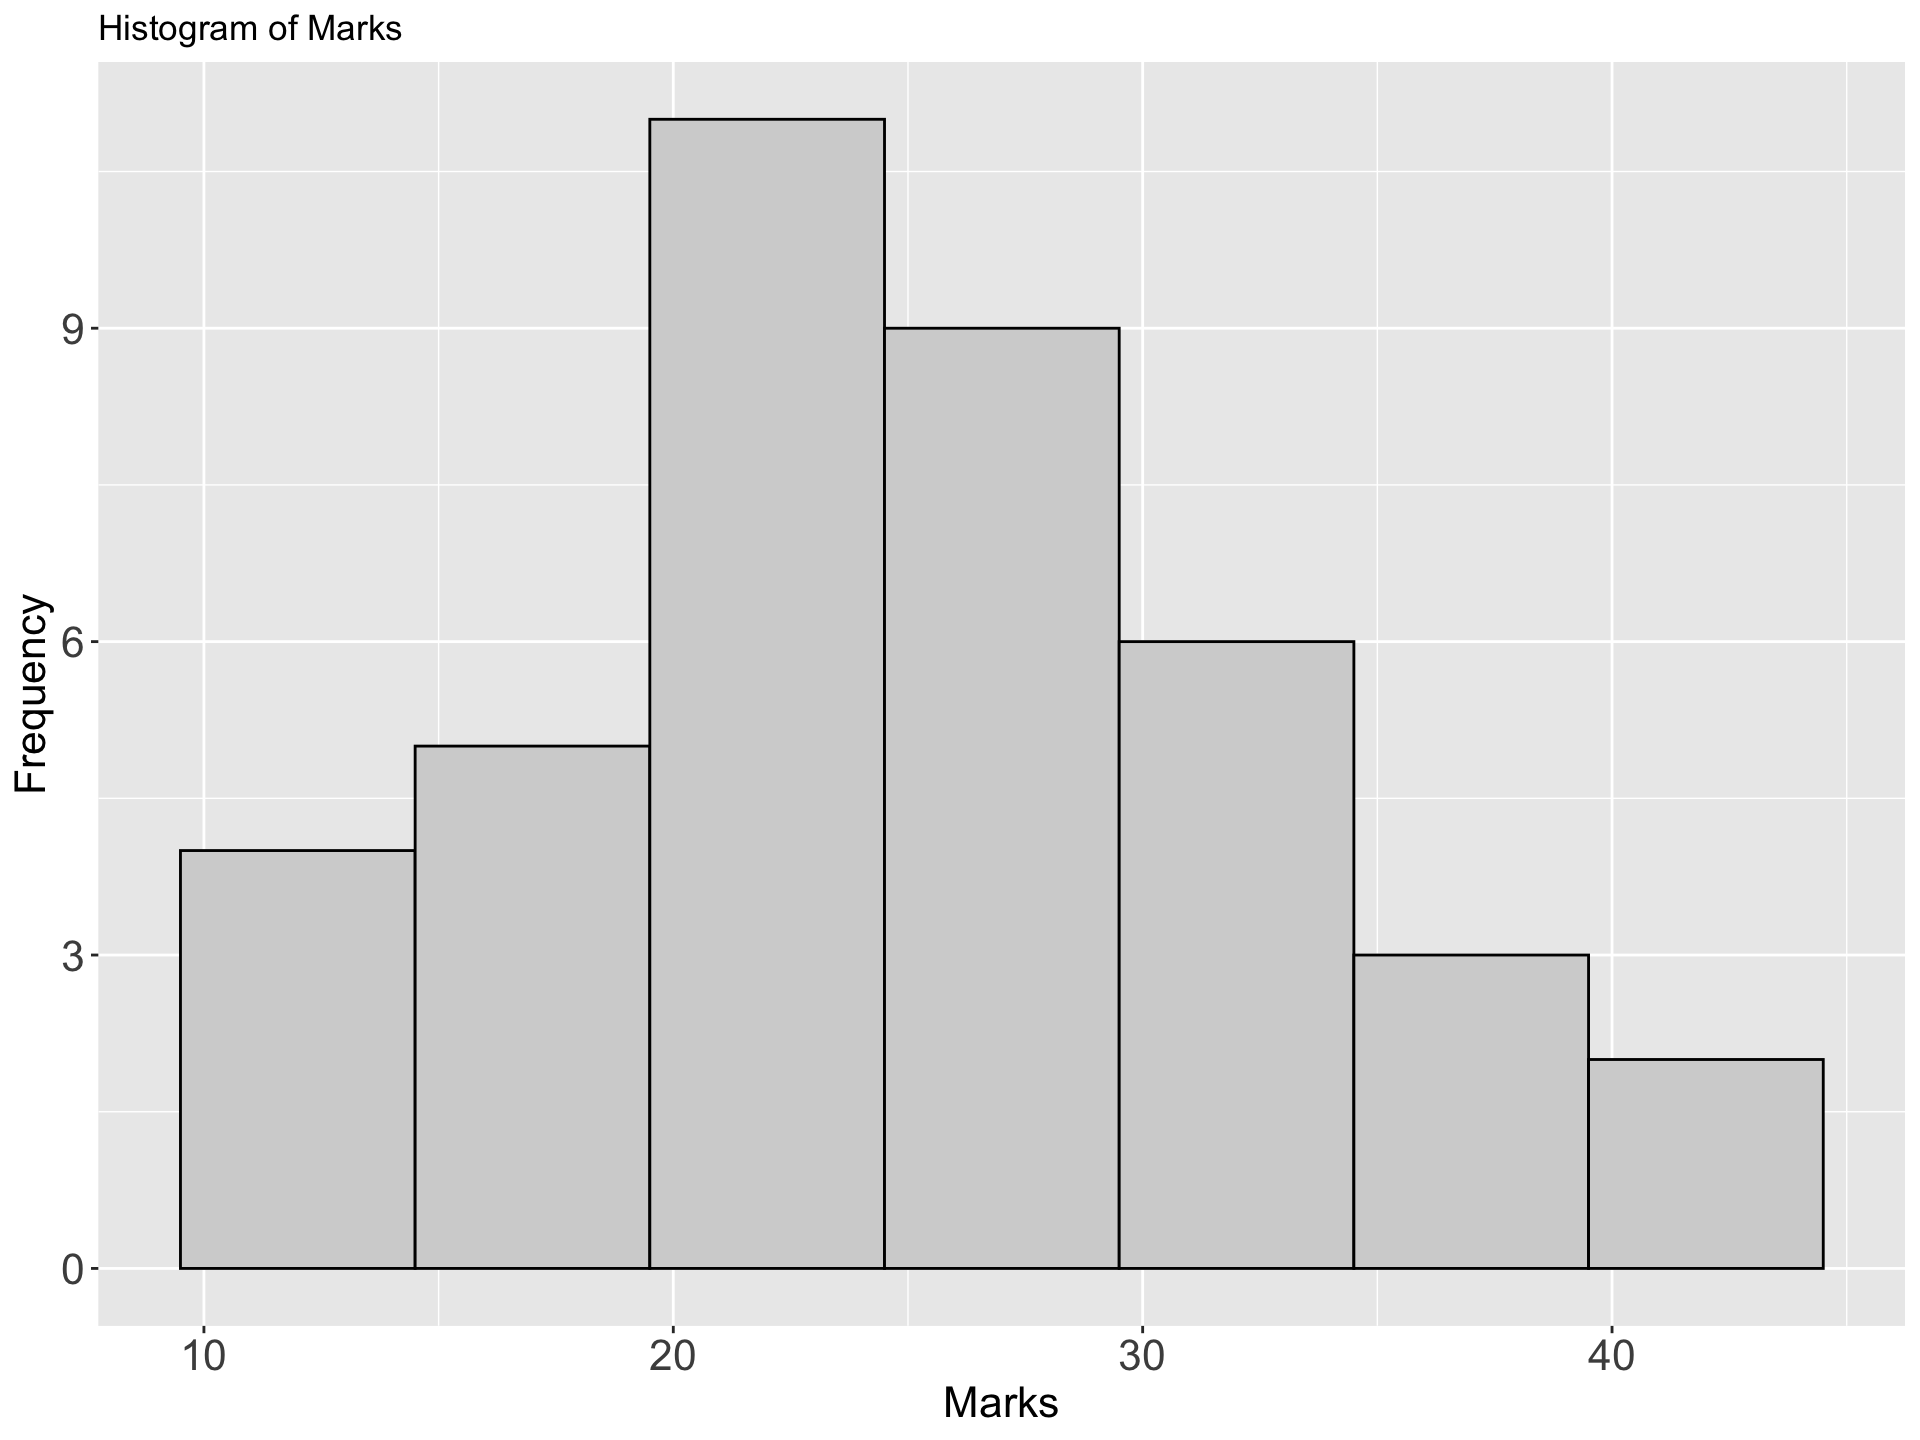
\includegraphics[width=0.8\linewidth]{figure/hist-1} \end{center}

Example 2

\begin{center}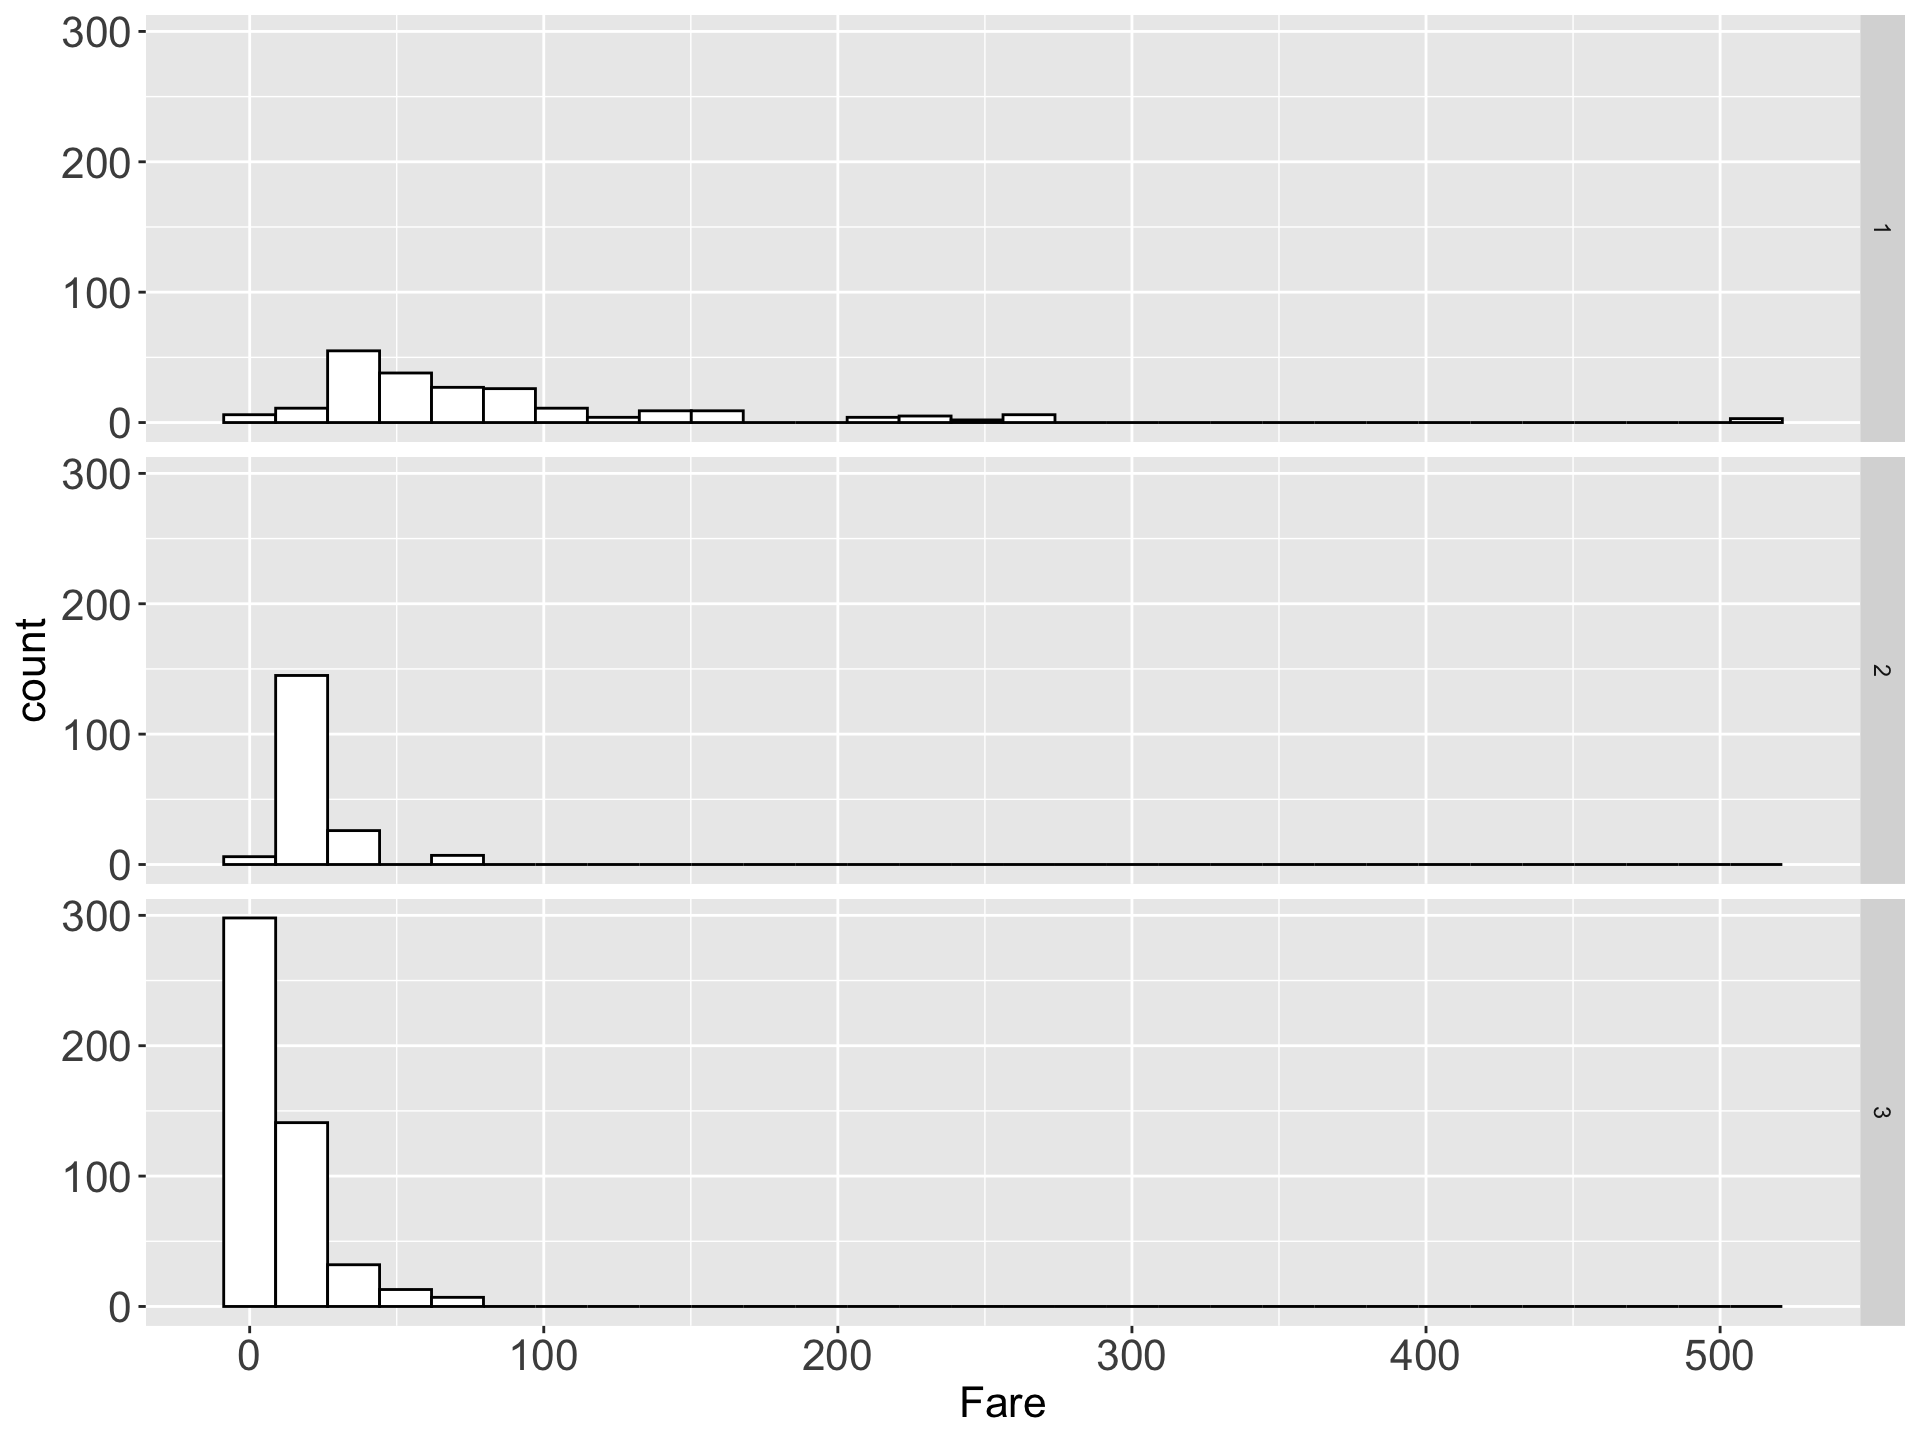
\includegraphics[width=0.8\linewidth]{figure/box18-1} \end{center}

\textbf{III Frequency polygon}

\begin{itemize}
\tightlist
\item
  If the mid-point of the top of each block in a histogram is joined by a straight line, a frequency polygon is produced.
\item
  This is done under the assumption that the frequencies in a class-interval are evenly distributed throughout the class
\end{itemize}

Example: The marks(out of 50) of a group of students are recorded in the accompanying table. Draw a frequency polygon for the data

\begin{longtable}[]{@{}ll@{}}
\toprule
Marks & Number of students\tabularnewline
\midrule
\endhead
10 - 14 & 4\tabularnewline
15 - 19 & 5\tabularnewline
20 - 24 & 11\tabularnewline
25 - 29 & 9\tabularnewline
30 - 34 & 6\tabularnewline
35 - 39 & 3\tabularnewline
40 - 44 & 2\tabularnewline
Total & 40\tabularnewline
\bottomrule
\end{longtable}

\begin{center}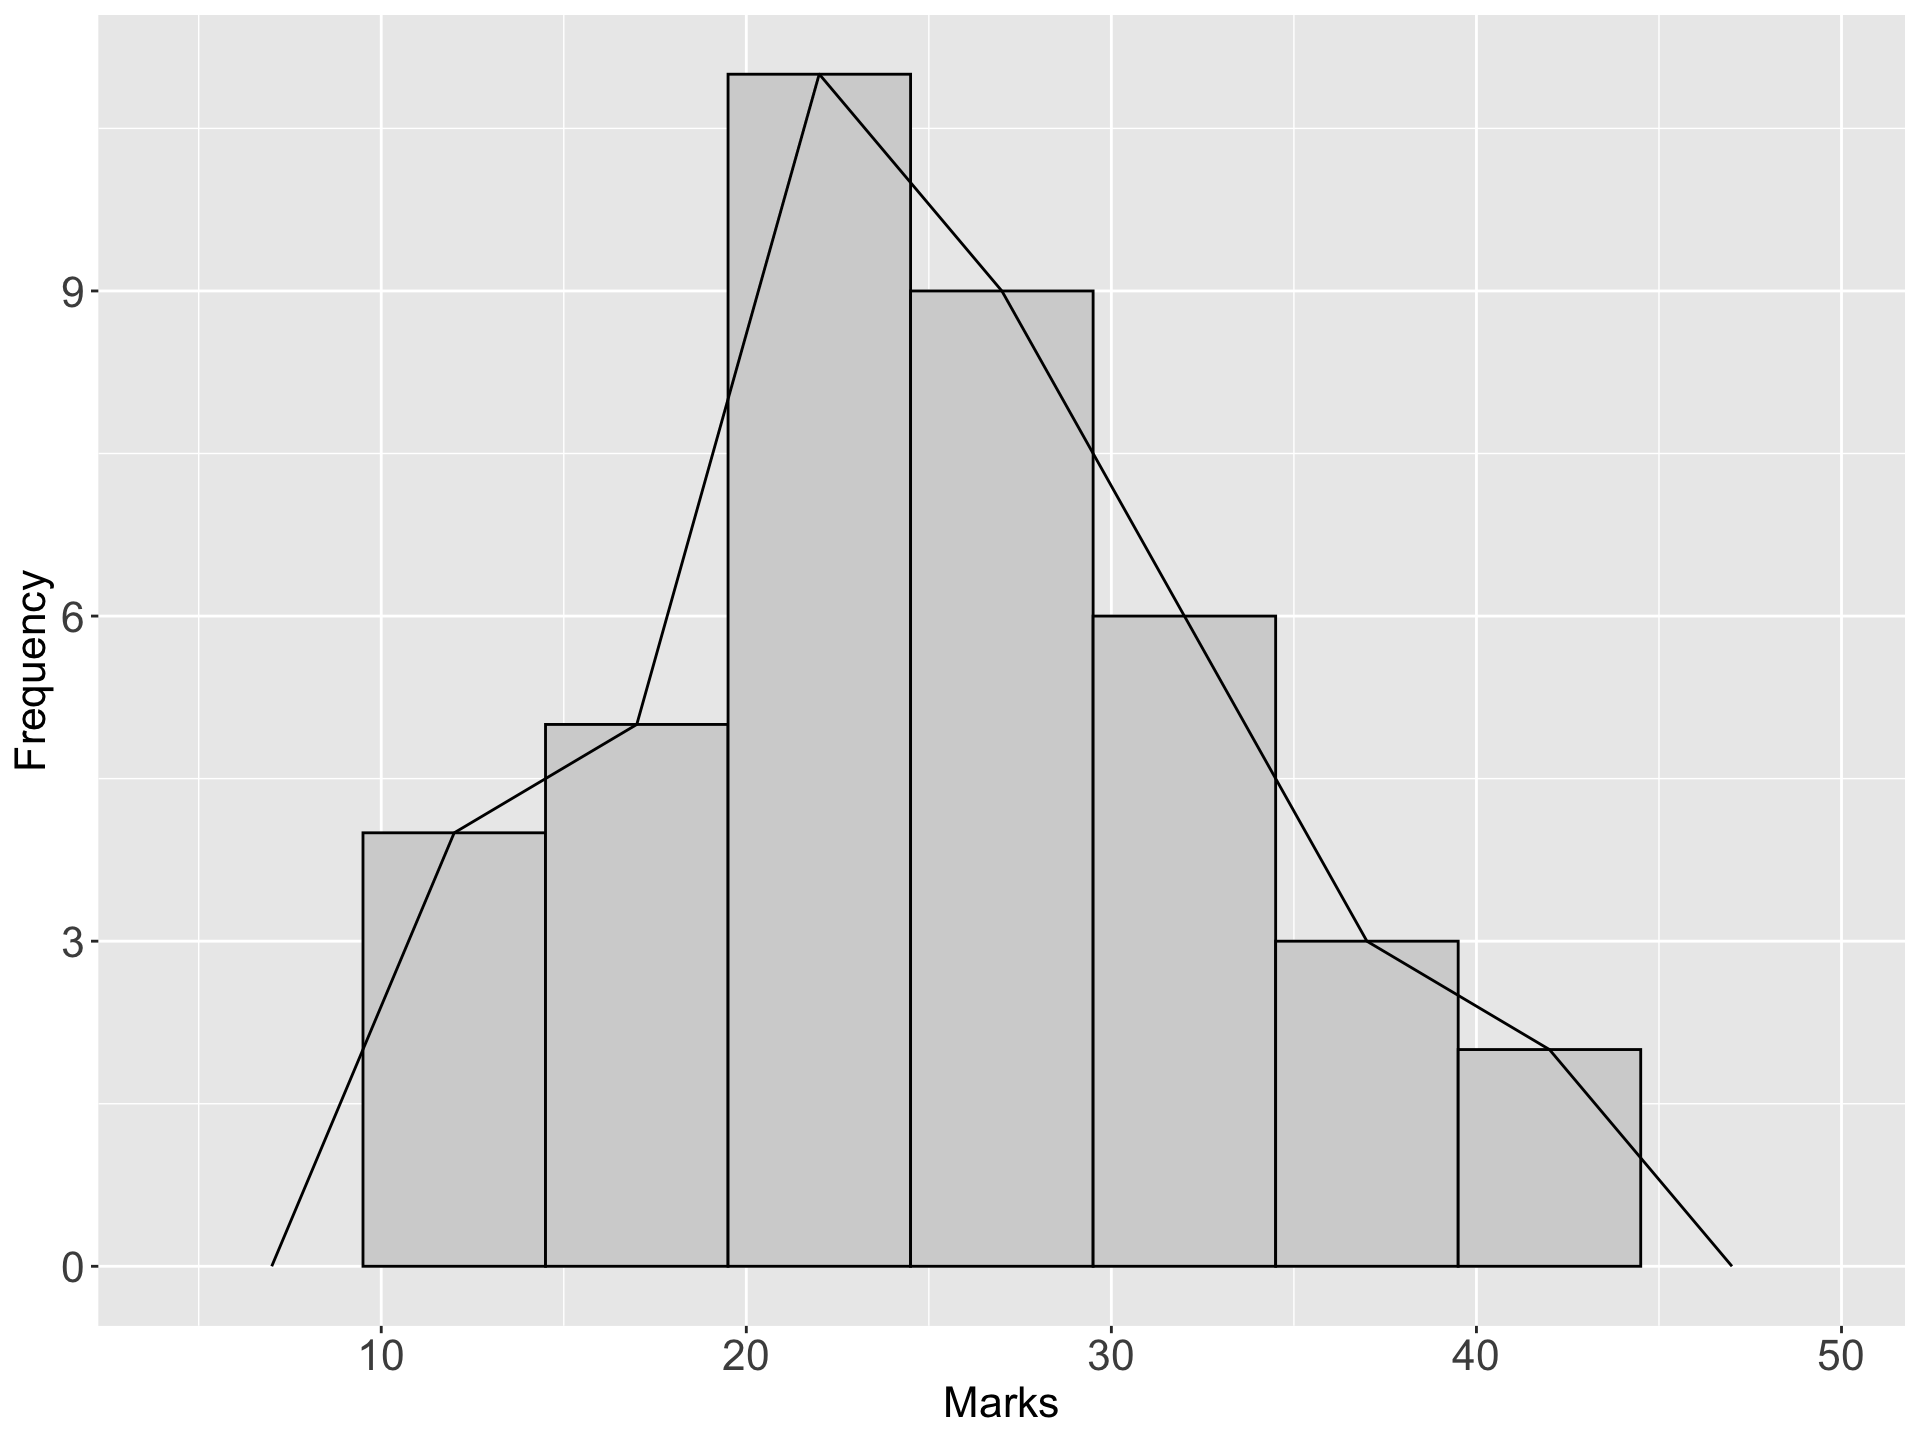
\includegraphics[width=0.8\linewidth]{figure/hist2-1} \end{center}

\textbf{IV Frequency curve}

\begin{itemize}
\tightlist
\item
  A frequency curve is drawn by smoothing the frequency polygon.
\item
  It is smooth in such a way that the sharp turns are avoided
\end{itemize}

Example: The marks(out of 50) of a group of students are recorded in the accompanying table. Draw a frequency curve for the data

\begin{longtable}[]{@{}ll@{}}
\toprule
Marks & Number of students\tabularnewline
\midrule
\endhead
10 - 14 & 4\tabularnewline
15 - 19 & 5\tabularnewline
20 - 24 & 11\tabularnewline
25 - 29 & 9\tabularnewline
30 - 34 & 6\tabularnewline
35 - 39 & 3\tabularnewline
40 - 44 & 2\tabularnewline
Total & 40\tabularnewline
\bottomrule
\end{longtable}

\begin{center}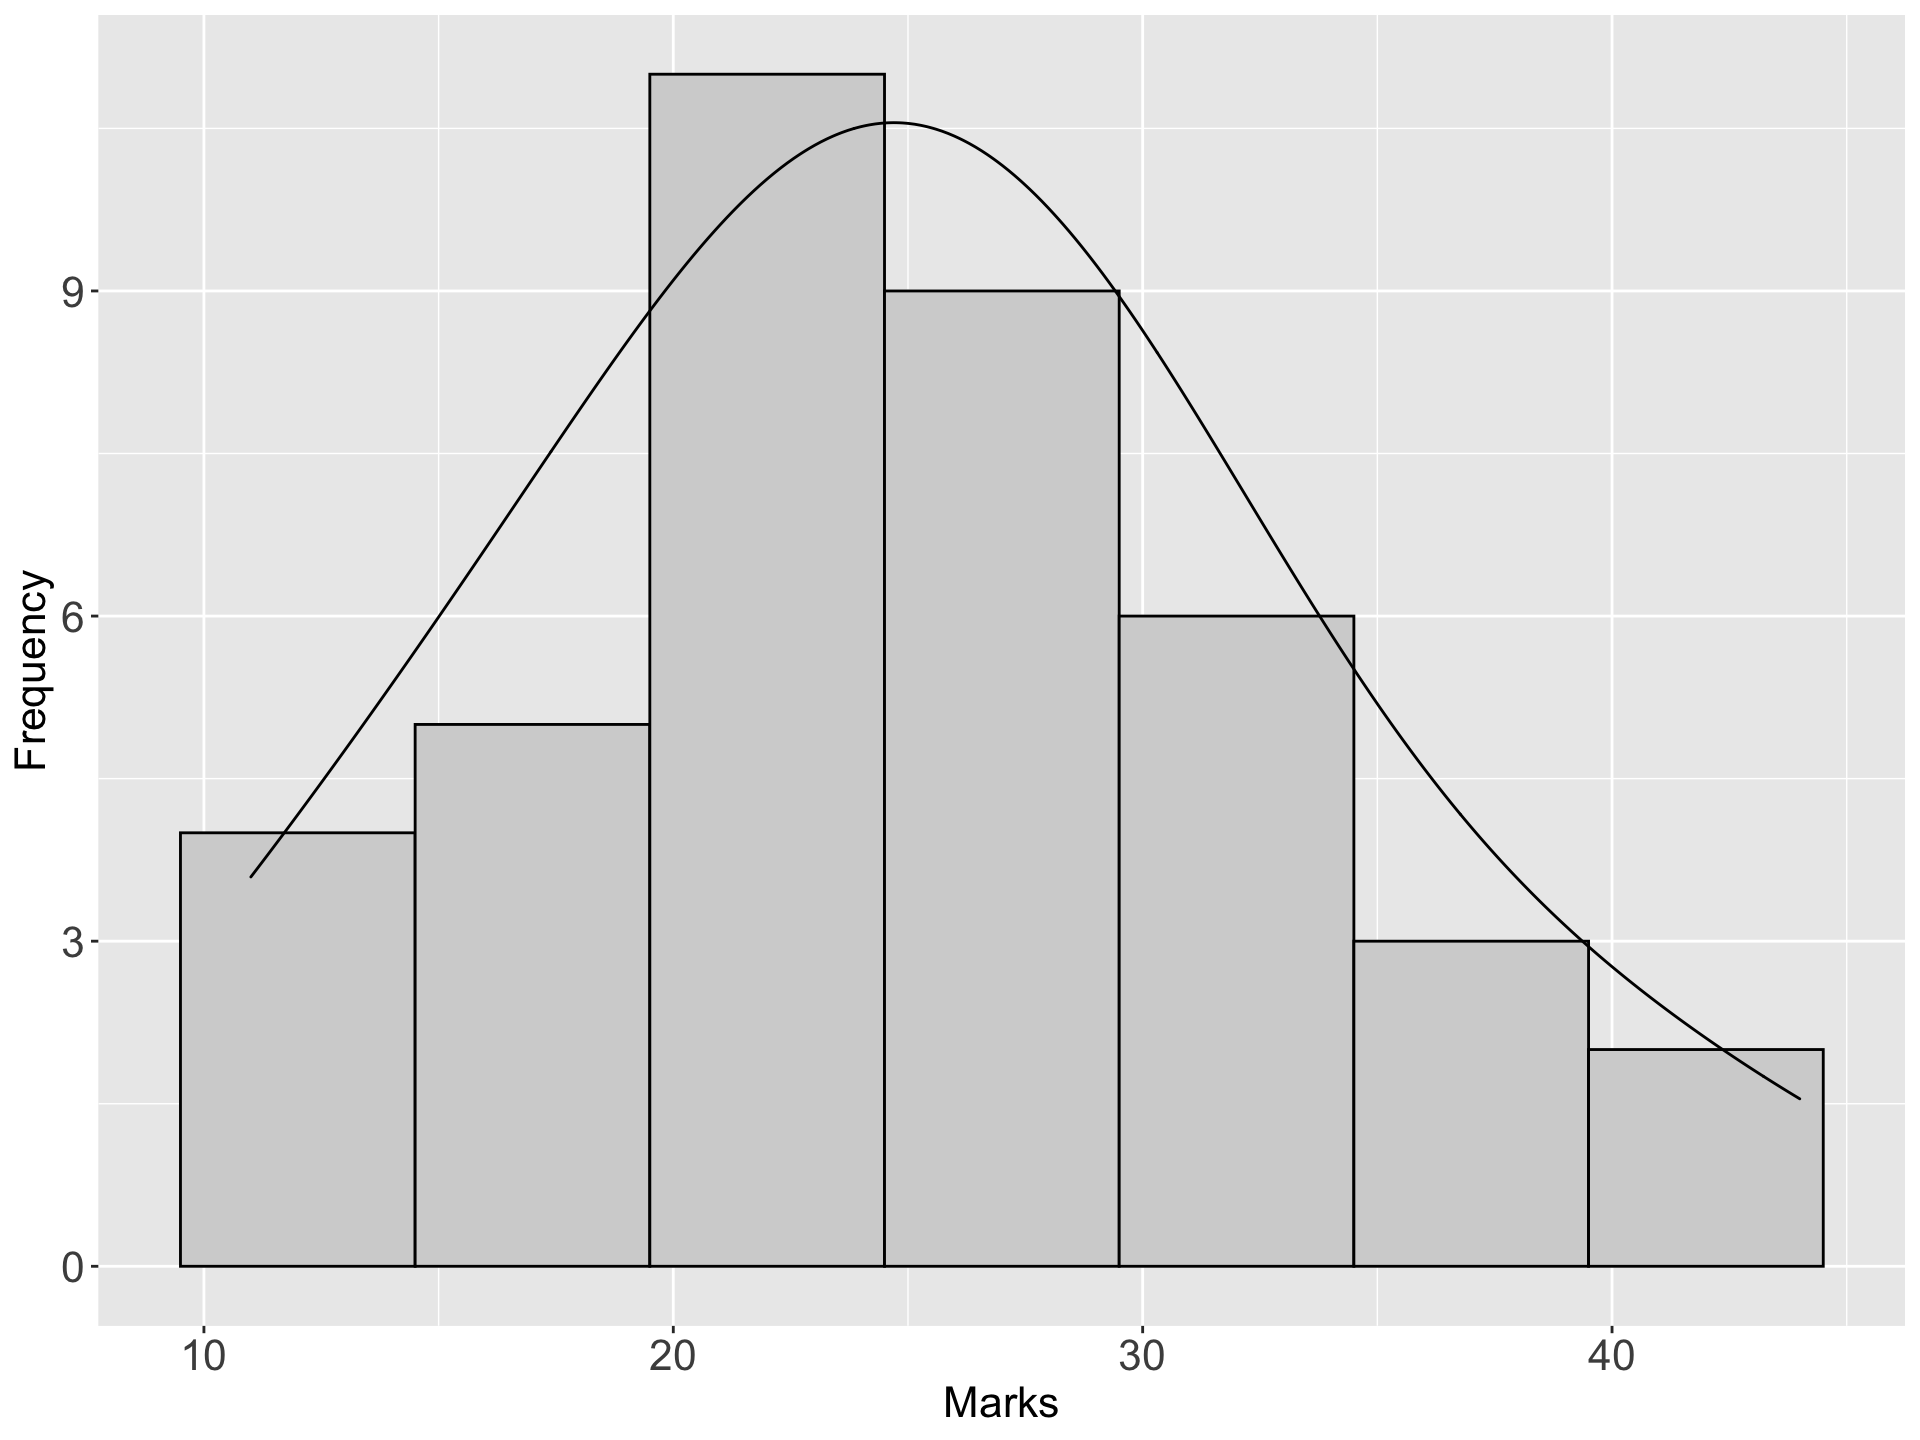
\includegraphics[width=0.8\linewidth]{figure/hist3-1} \end{center}

frequency curves arising in practice take on certain characteristics shapes as shown bellow

\begin{center}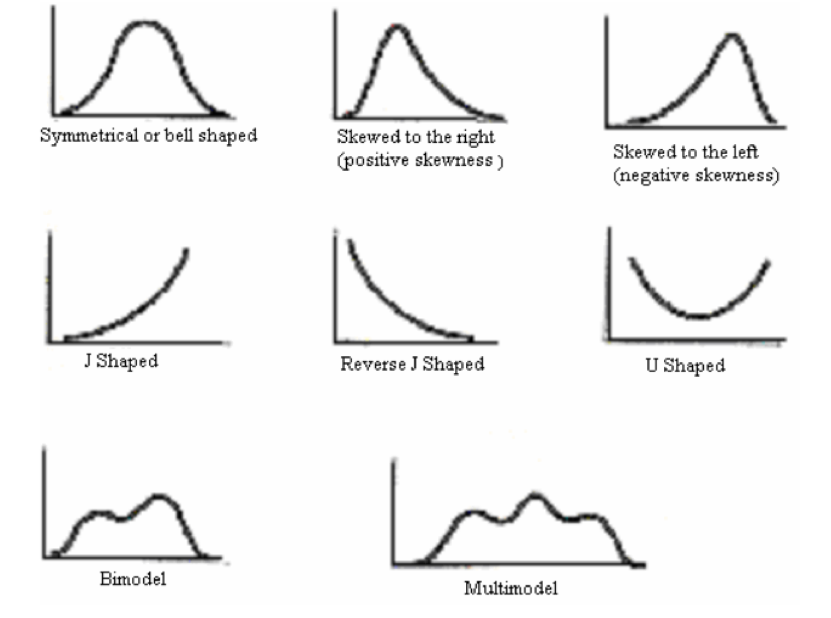
\includegraphics[width=1\linewidth]{figure/shapes} \end{center}

\begin{enumerate}
\def\labelenumi{\arabic{enumi}.}
\tightlist
\item
  The \textbf{symmetrical} or \textbf{bell shaped} frequency curves are characterized by the fact that observations equidistant from the central maximum have the same frequency. An important example is the normal curve.
\item
  In the \textbf{moderately asymmetrical} or \textbf{skewed} frequency curves the tail of the curve to one side of the central maximum is longer than that to the other. If the longer tail occurs to the right the curve is said to be \textbf{skewed to the right} or to have \textbf{positive skewness}.While if the reverse is true the curve is said to be \textbf{skewed to the left} or to have \textbf{negative skewness}.
\item
  In a \textbf{J shaped} or \textbf{reverse J shaped} curve a maximum occurs at one end.
\item
  A \textbf{U shaped} frequency curve has maxima at both ends.
\item
  A \textbf{bimodal} frequency curve has two maxima. These appear as two distinct peaks (local maxima) in the frequency curve.When the two modes are unequal the larger mode is known as the major mode and the other as the minor mode.
\item
  A \textbf{multimodal} frequency curve has more than two maxima.
\end{enumerate}

\textbf{V Dot Plot}

\begin{itemize}
\tightlist
\item
  A dot plot is a method of presenting data which gives a rough but rapid visual appreciation of the way in which the data are distributed
\item
  It consists of a horizontal line marked out with divisions of the scale on which the variable is being measured
  -This graph can be used to represent only the numerical data.
\end{itemize}

\begin{center}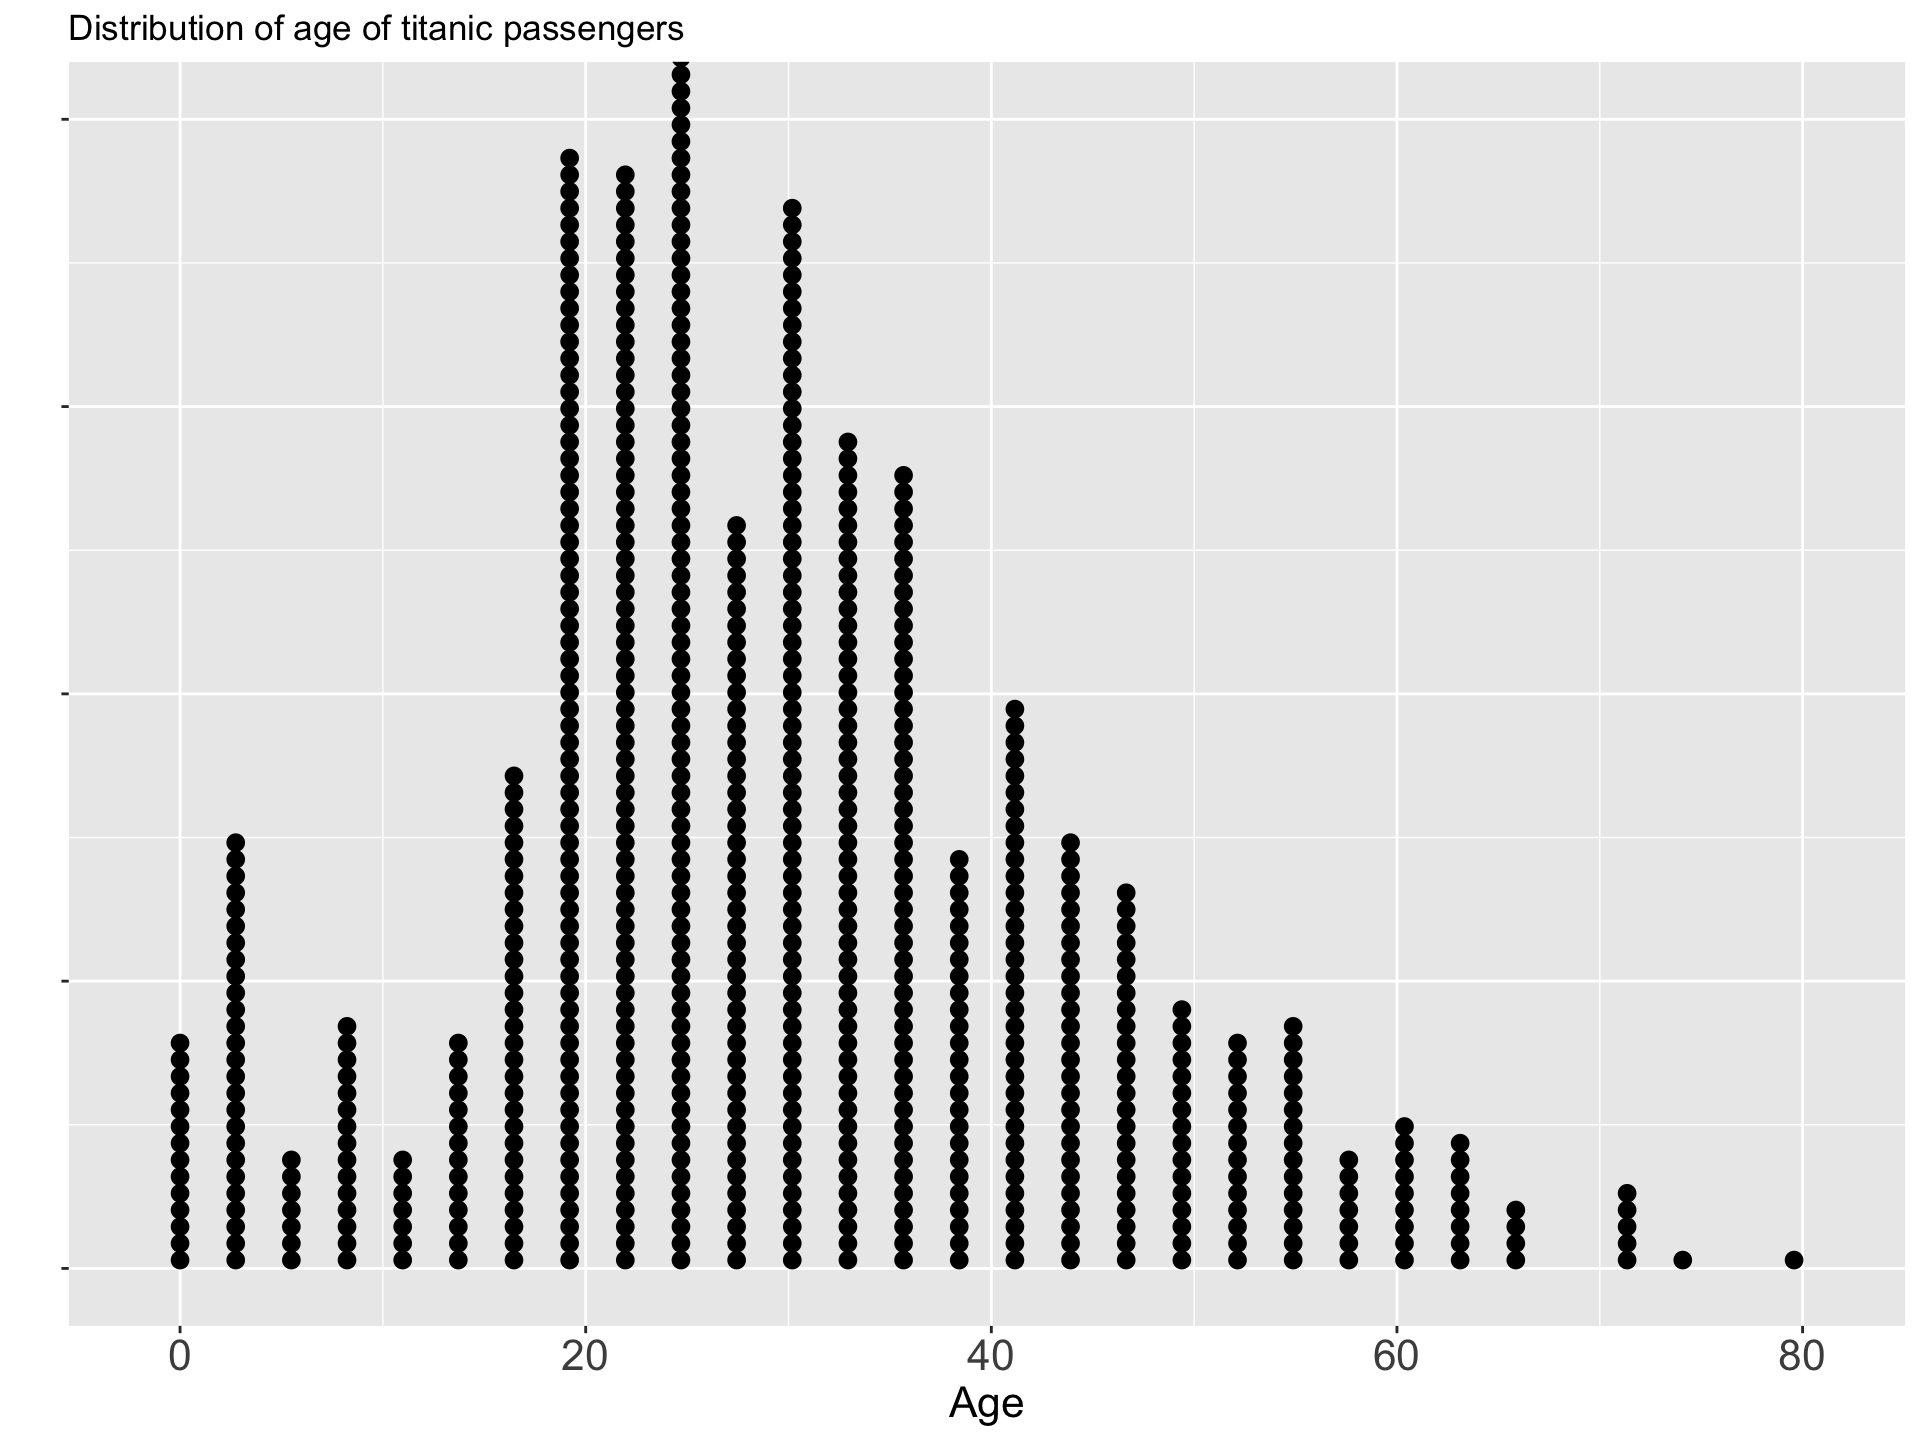
\includegraphics[width=0.8\linewidth]{figure/dotplot-1} \end{center}

\textbf{VI Box plot (Box and whisker plot)}

\begin{itemize}
\tightlist
\item
  Box plot is also a useful method of representing the behavior of a data set or comparing two or more data sets.
\item
  Box plot is constructed by identifying five statistics from the data set as largest value, smallest values, median, Q1 and Q3.
\end{itemize}

\begin{center}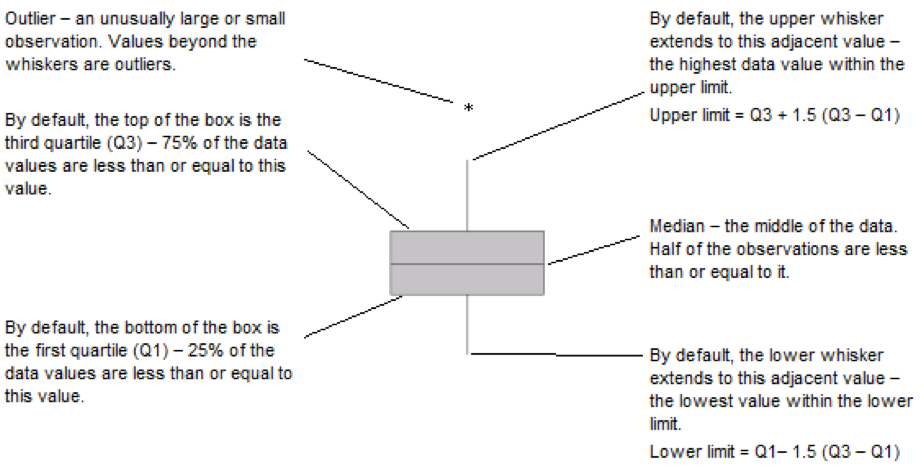
\includegraphics[width=1\linewidth]{figure/boxplot} \end{center}

Example:

Construct a box plot for the following data set (Marks of students)

\[\text{52, 88, 56, 79, 72, 91,  85, 88, 68, 63, 76, 73, 86, 95, 12, 69}\]

Xmin = 12 Xmax = 95 Q1 =64.25 Q2 = Median = 74.5 Q3 = 87.5

\begin{center}
\includegraphics[width=1\linewidth]{figure/box61-1} \end{center}

\begin{center}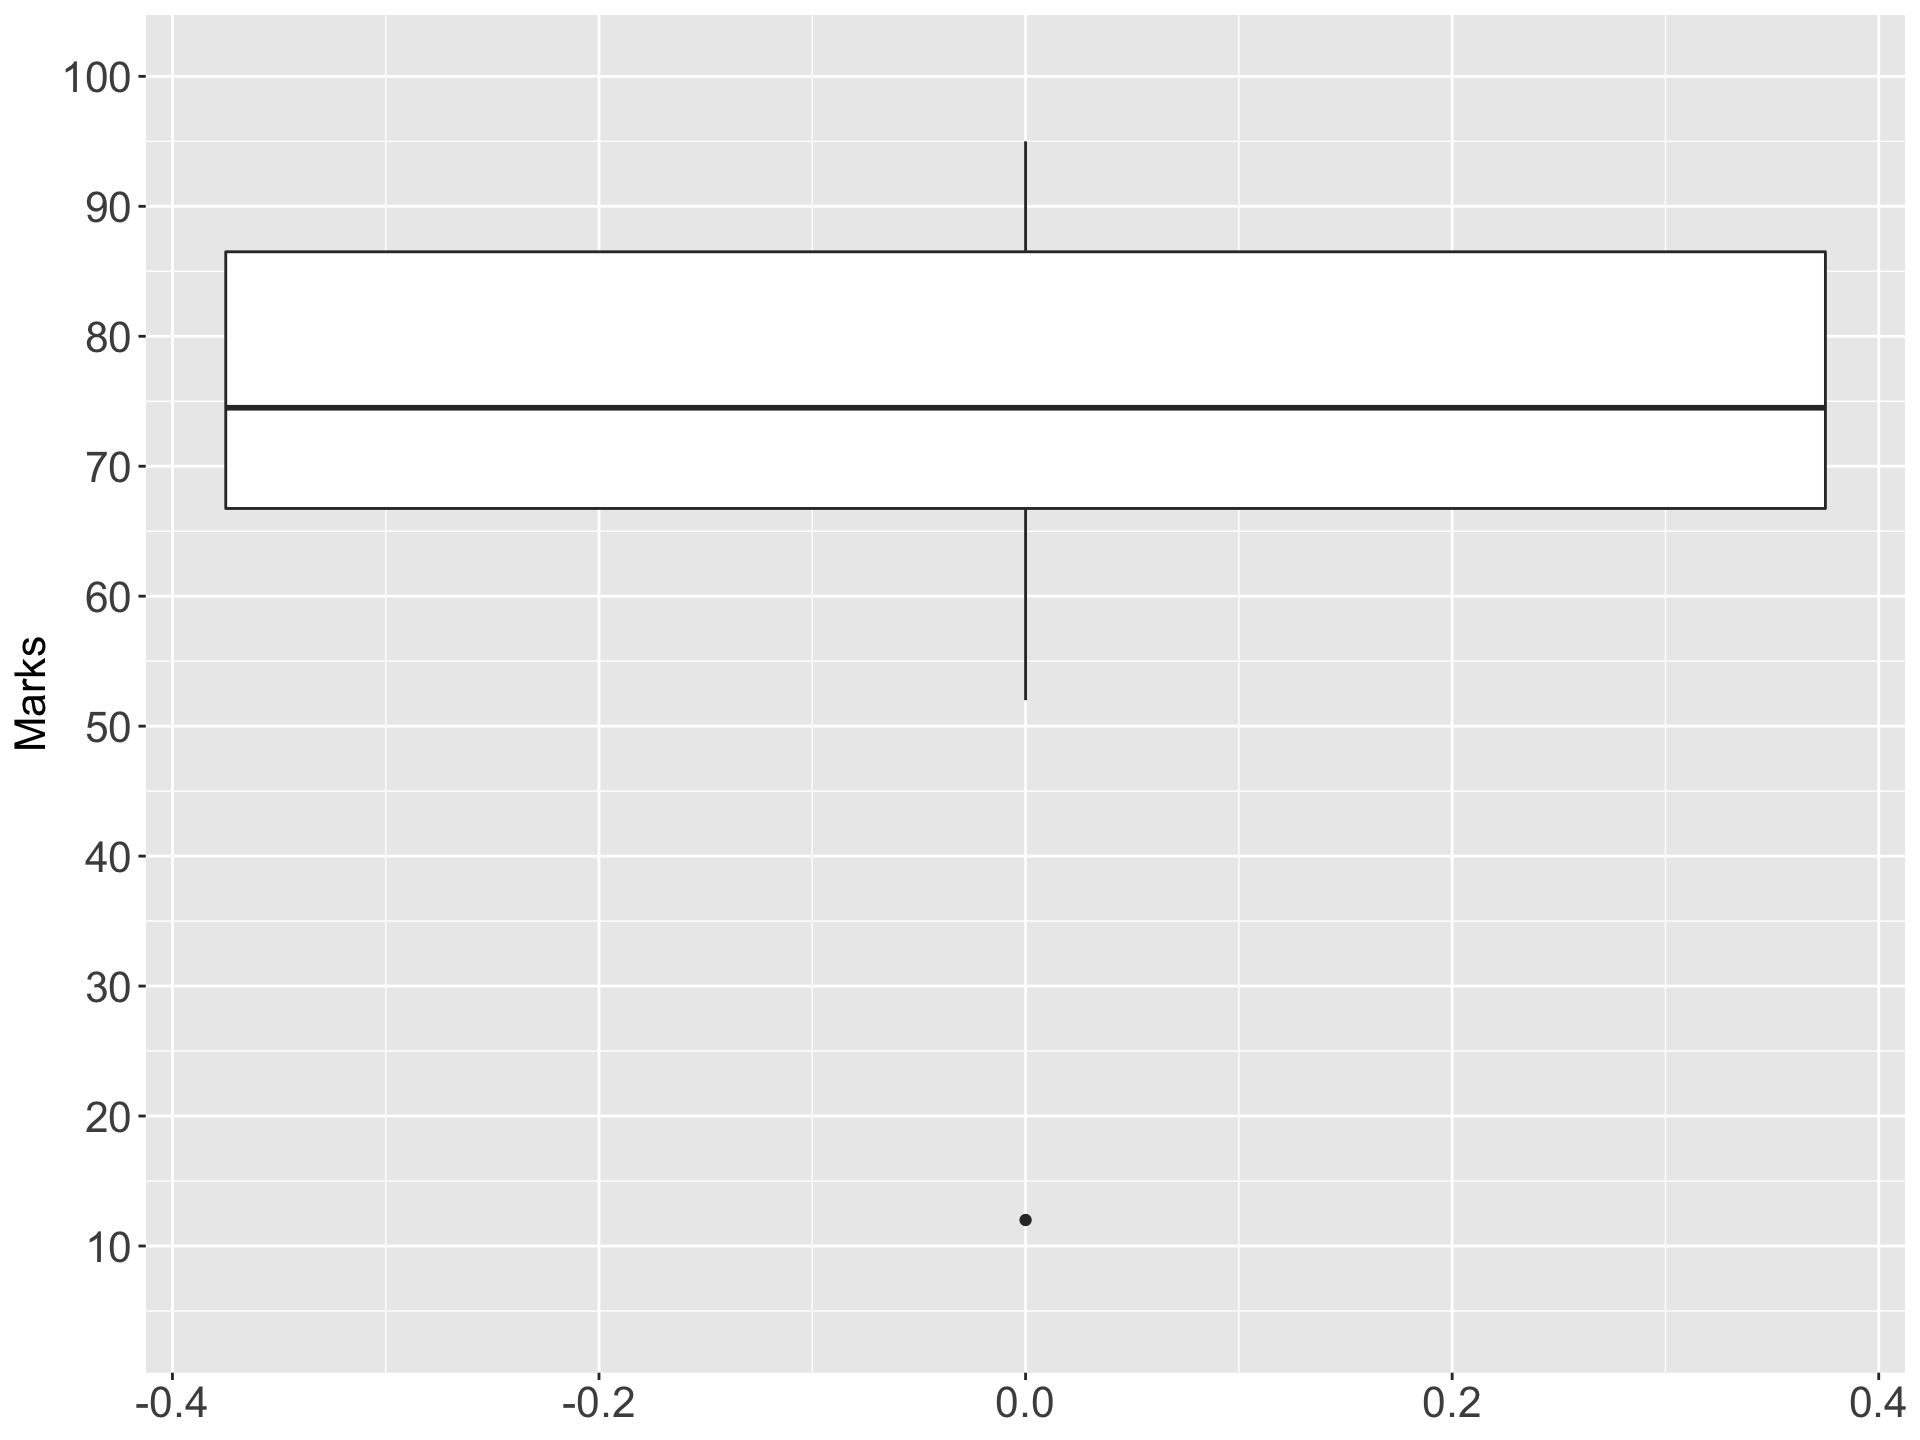
\includegraphics[width=0.8\linewidth]{figure/boxplot-1} \end{center}

\begin{center}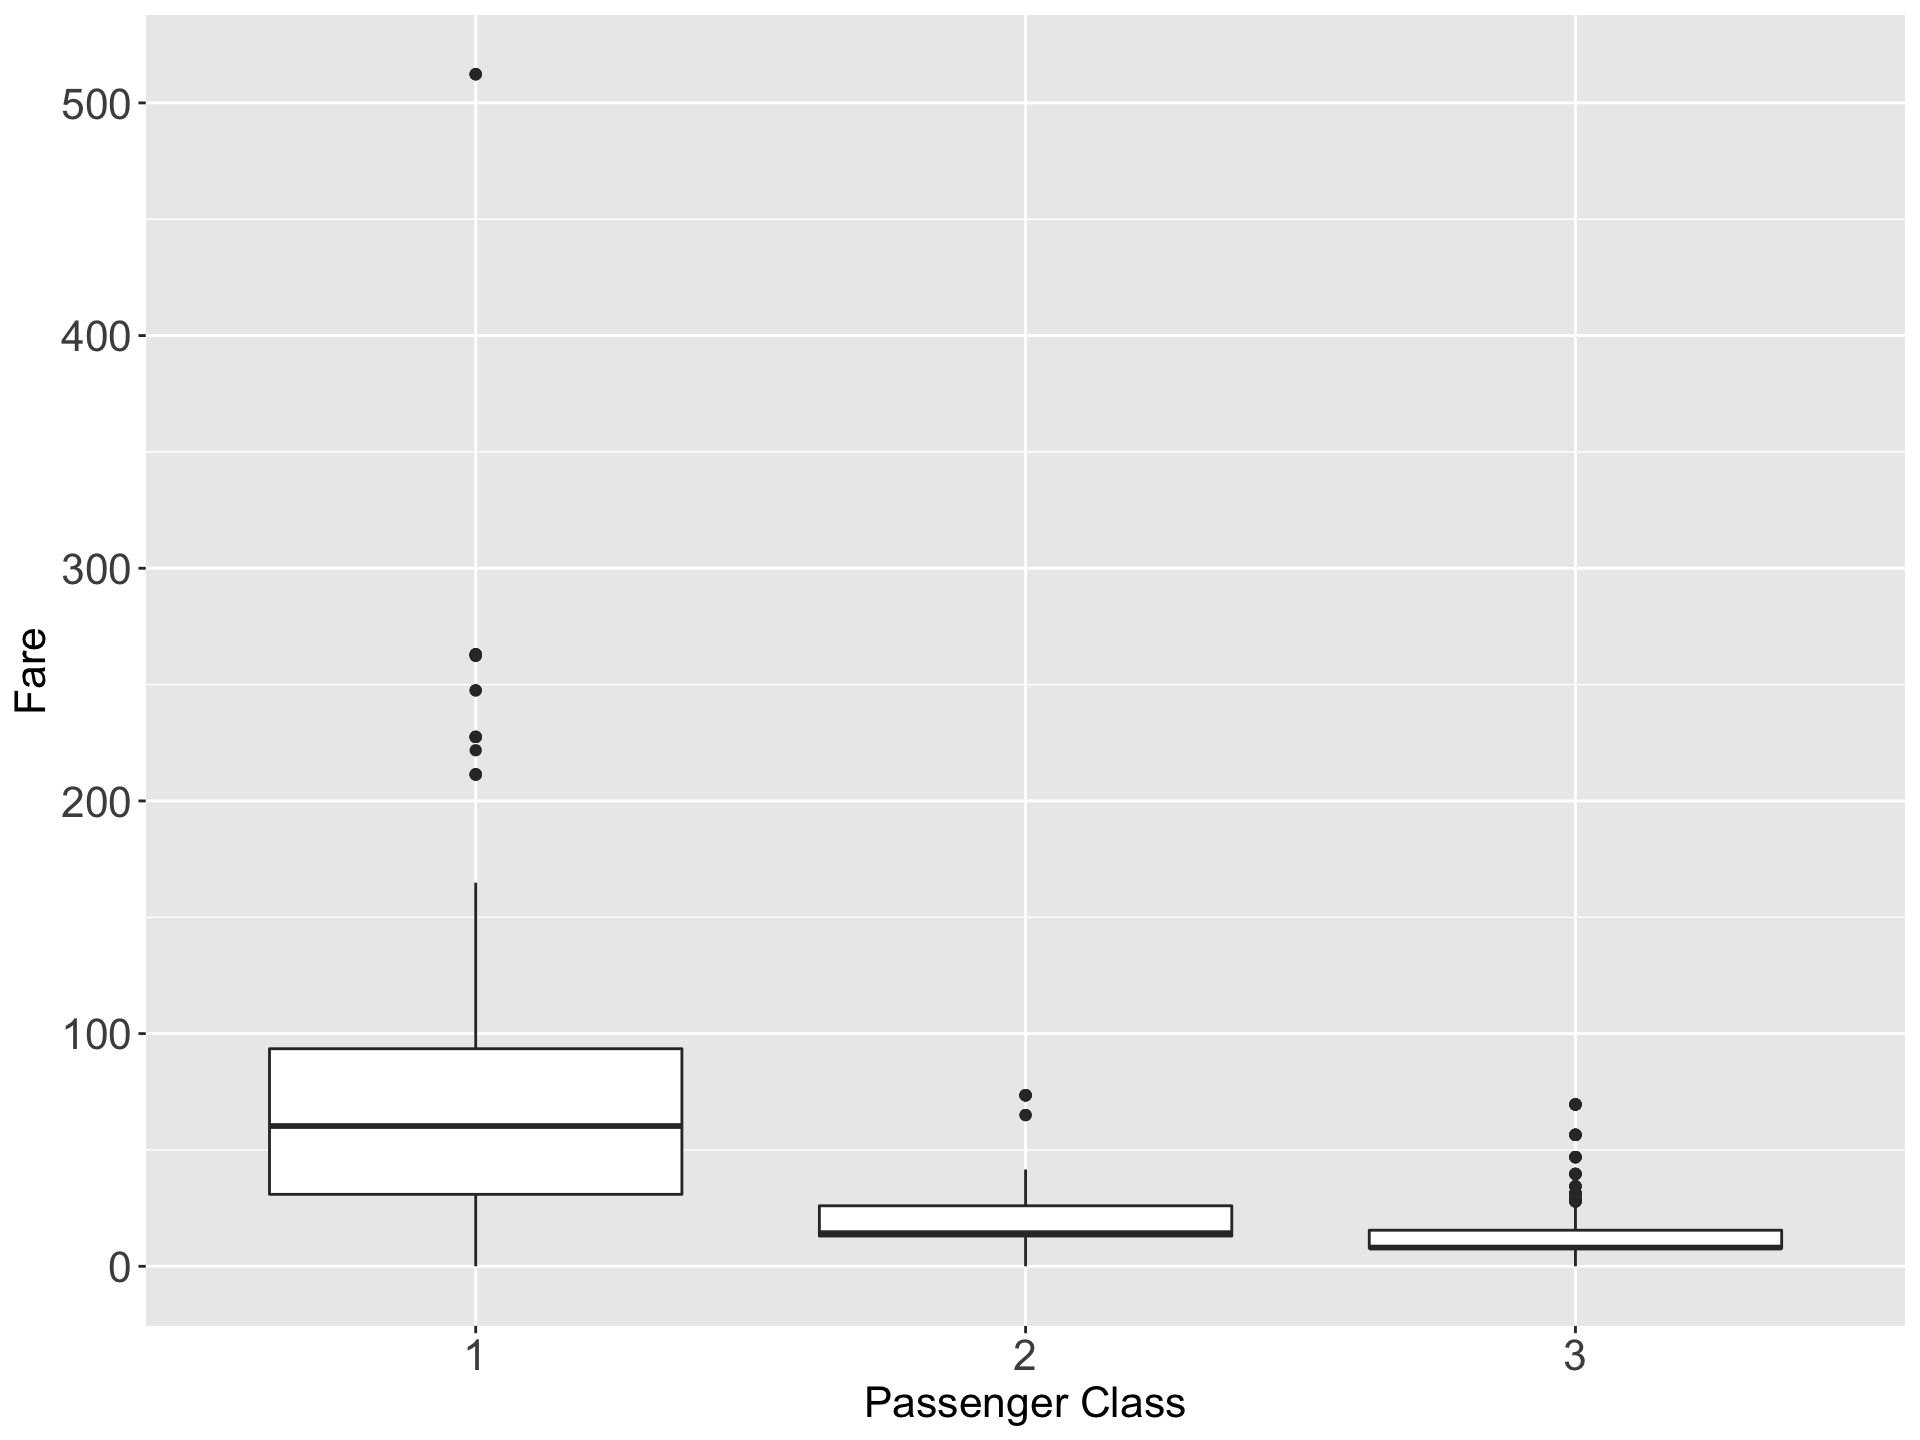
\includegraphics[width=0.8\linewidth]{figure/boxplot2-1} \end{center}

\begin{center}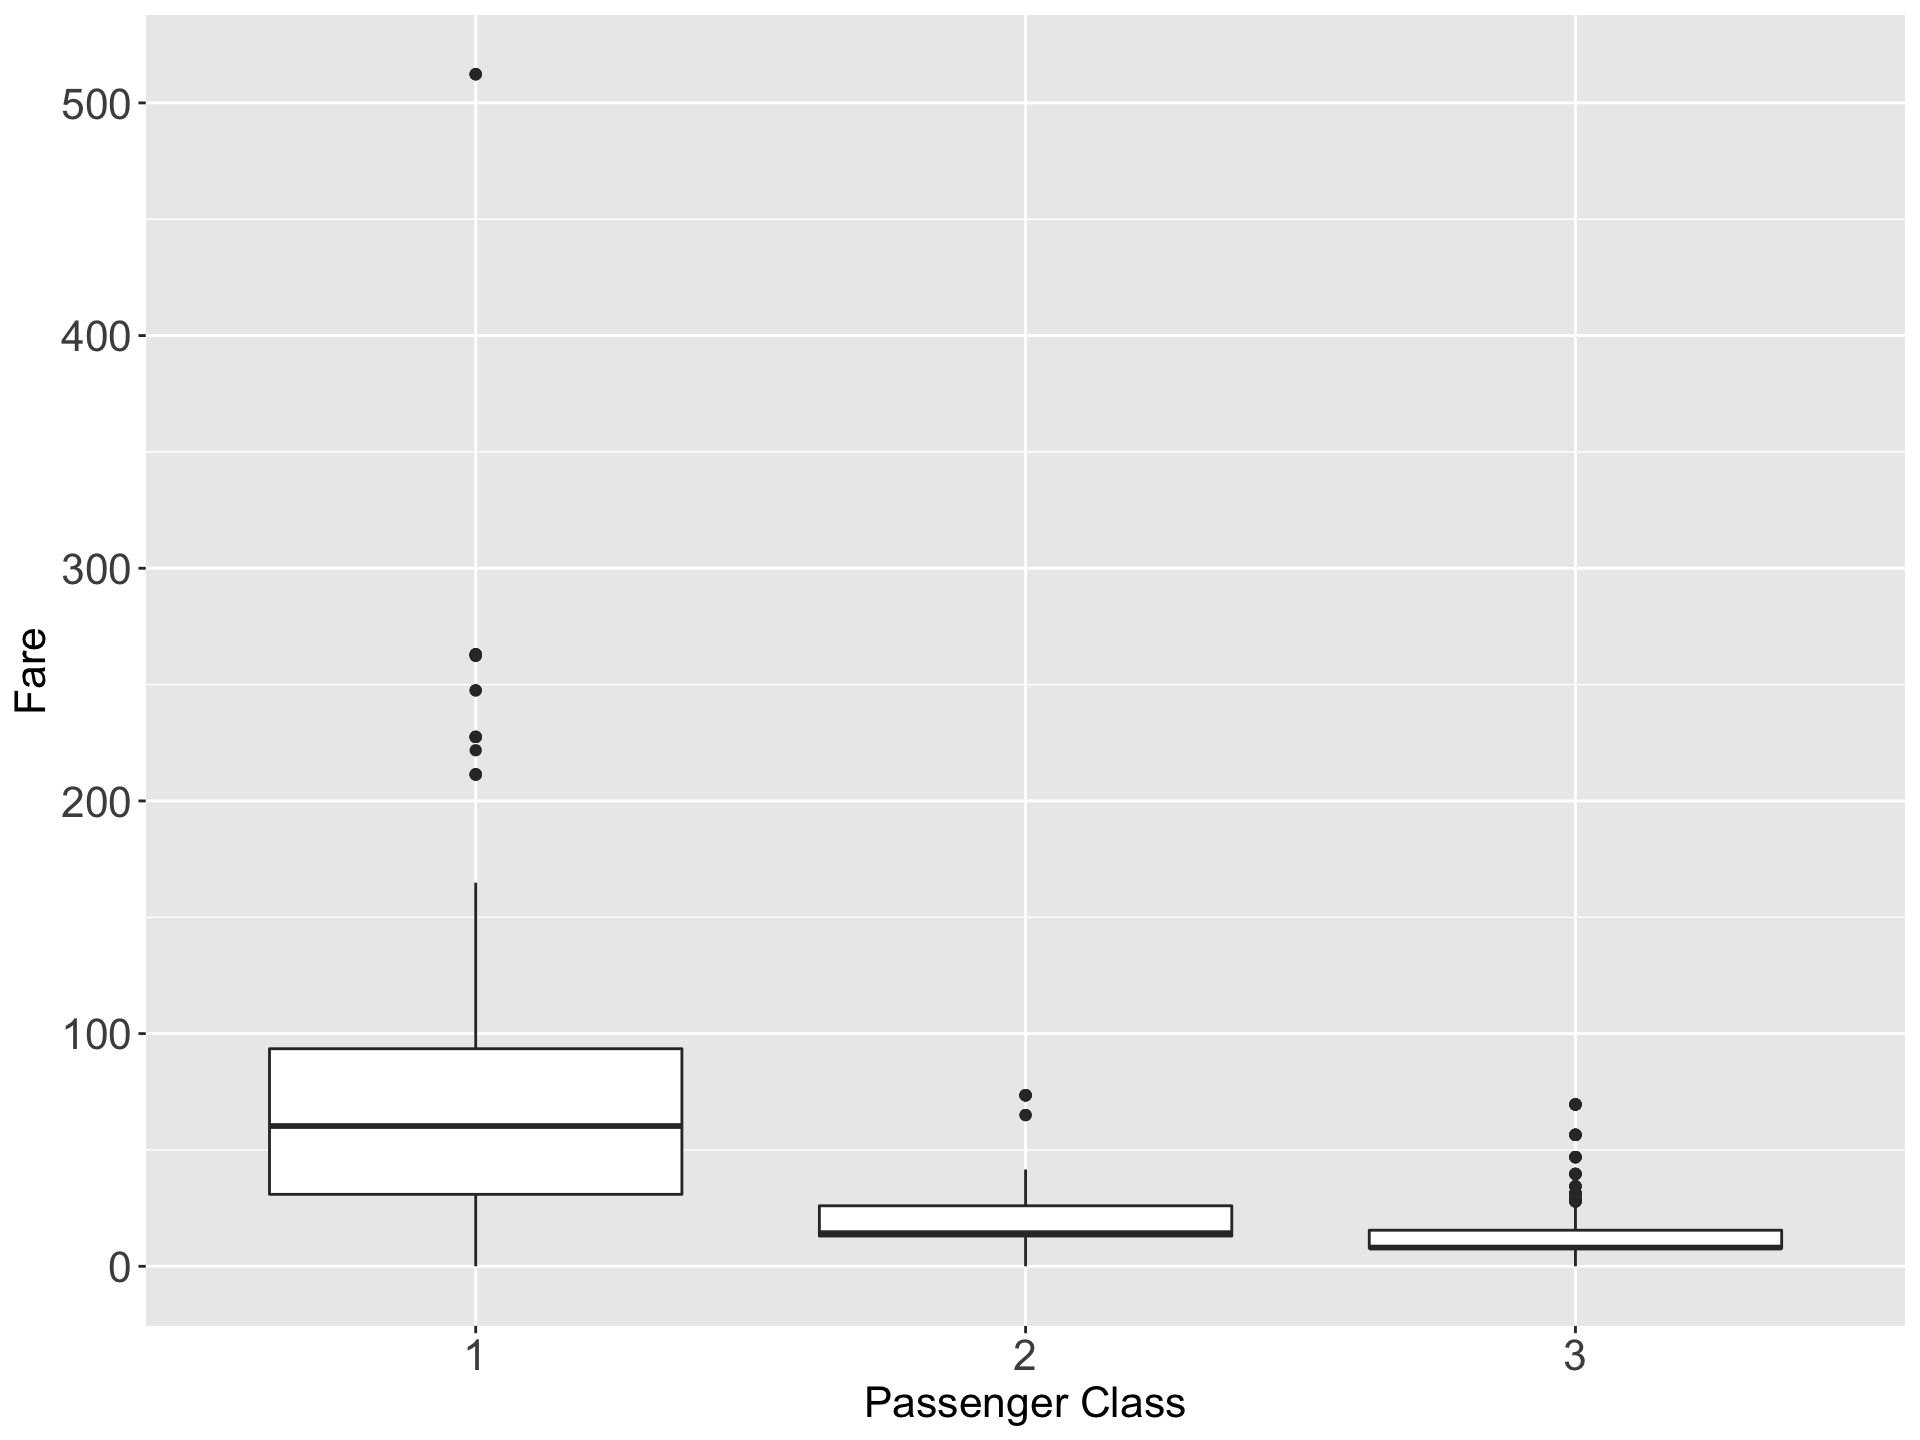
\includegraphics[width=0.8\linewidth]{figure/boxplot3-1} \end{center}

\textbf{VII Violin plot}

\begin{itemize}
\tightlist
\item
  A violin plot is a method of plotting quantitative data.
\item
  It is similar to a box plot, with the addition of a rotated kernel density plot on each side.
\item
  Violin plots are similar to box plots, except that they also show the probability density of the data at different values, usually smoothed by a kernel density estimator.
\end{itemize}

\begin{center}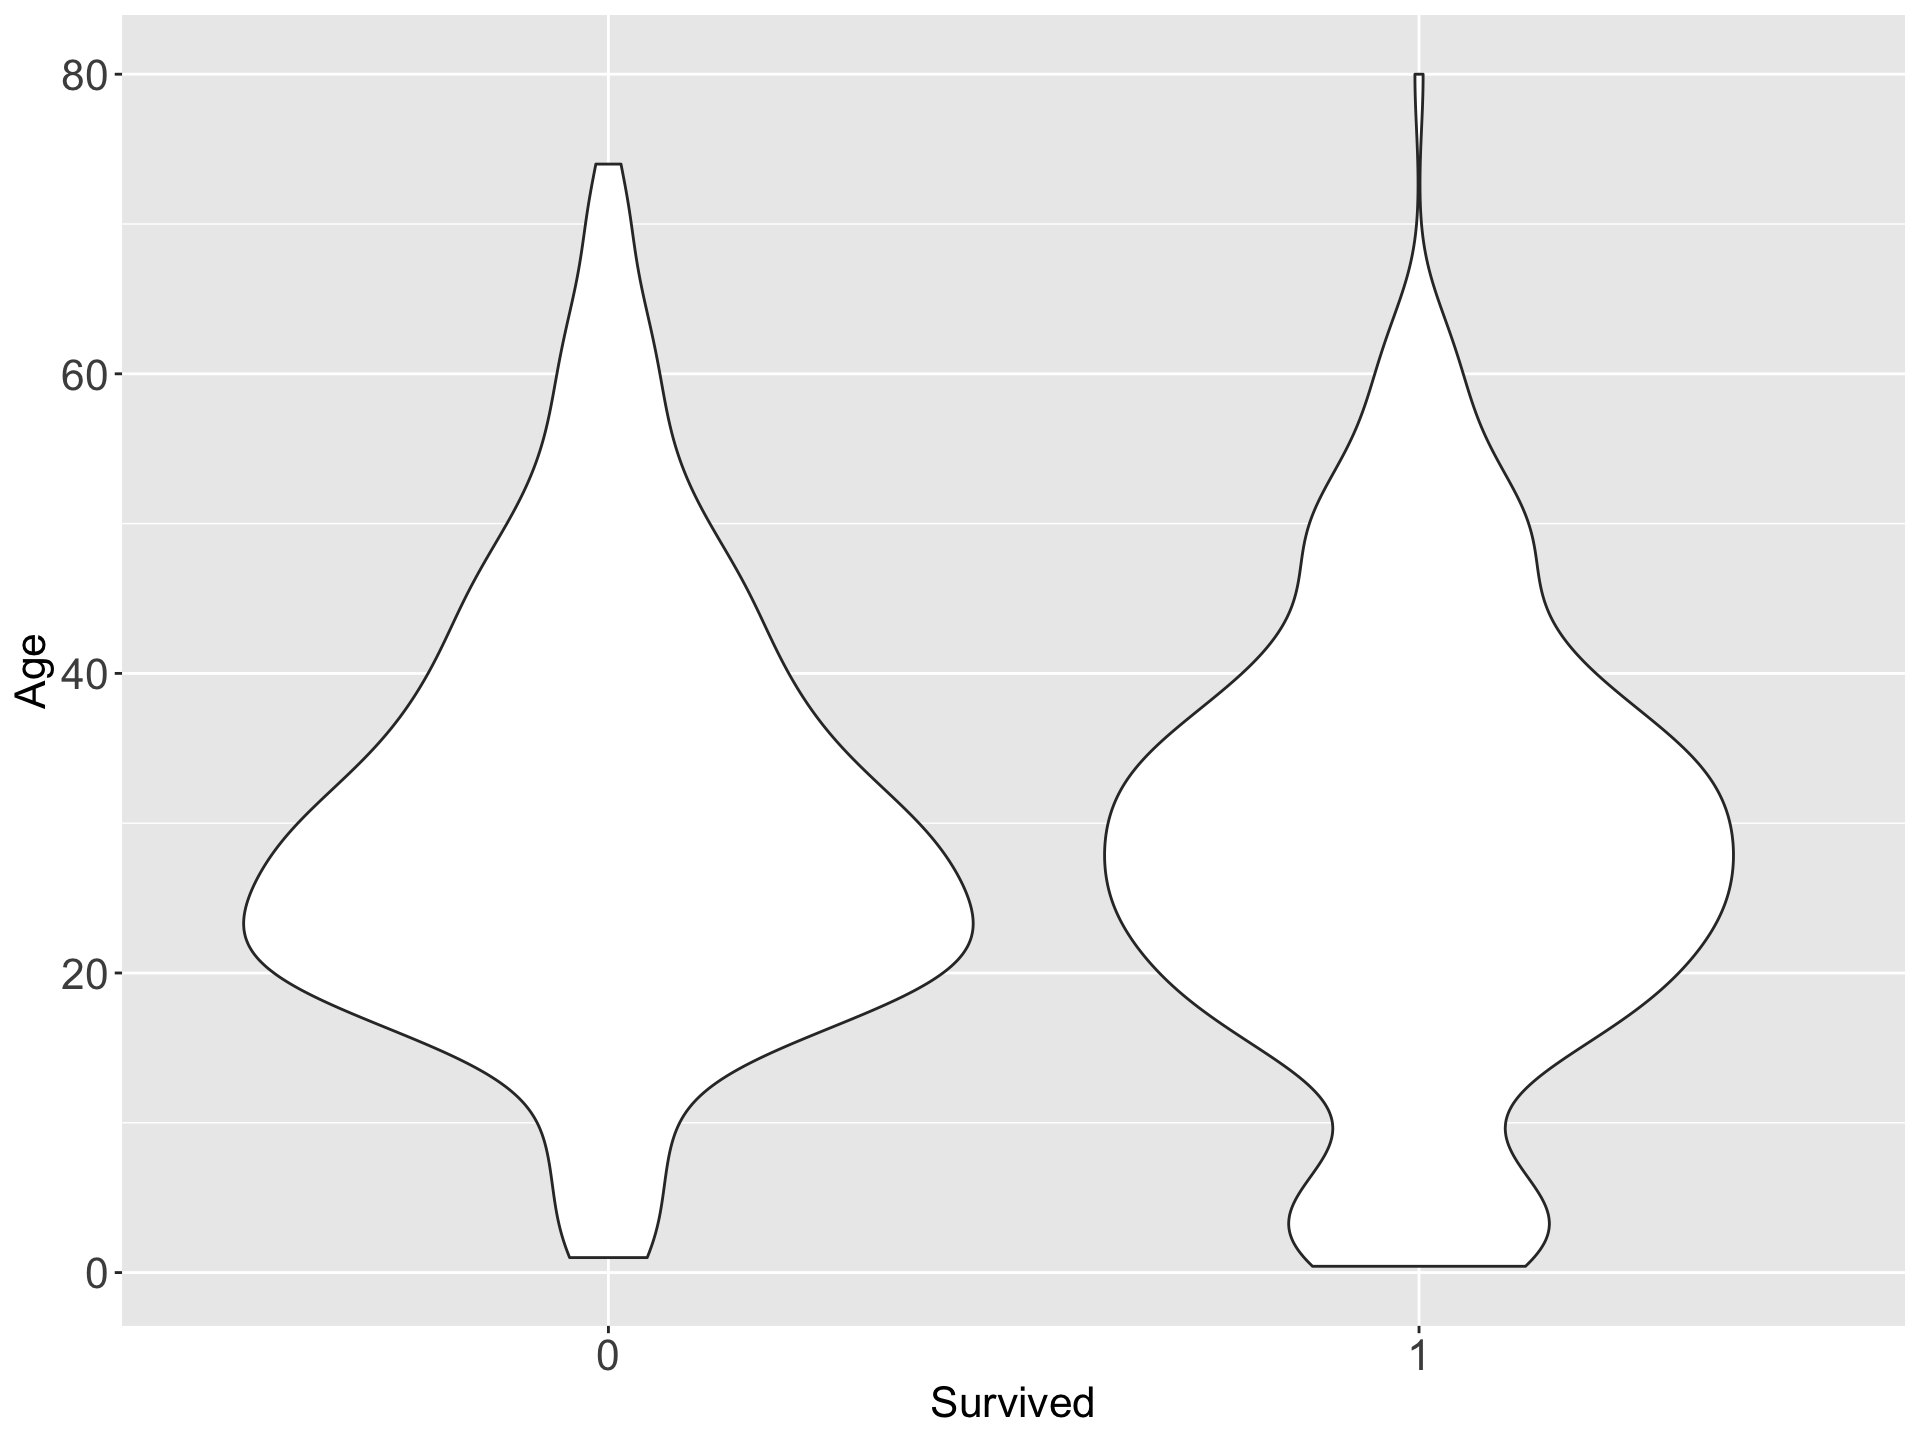
\includegraphics[width=0.8\linewidth]{figure/violin1-1} \end{center}

\begin{center}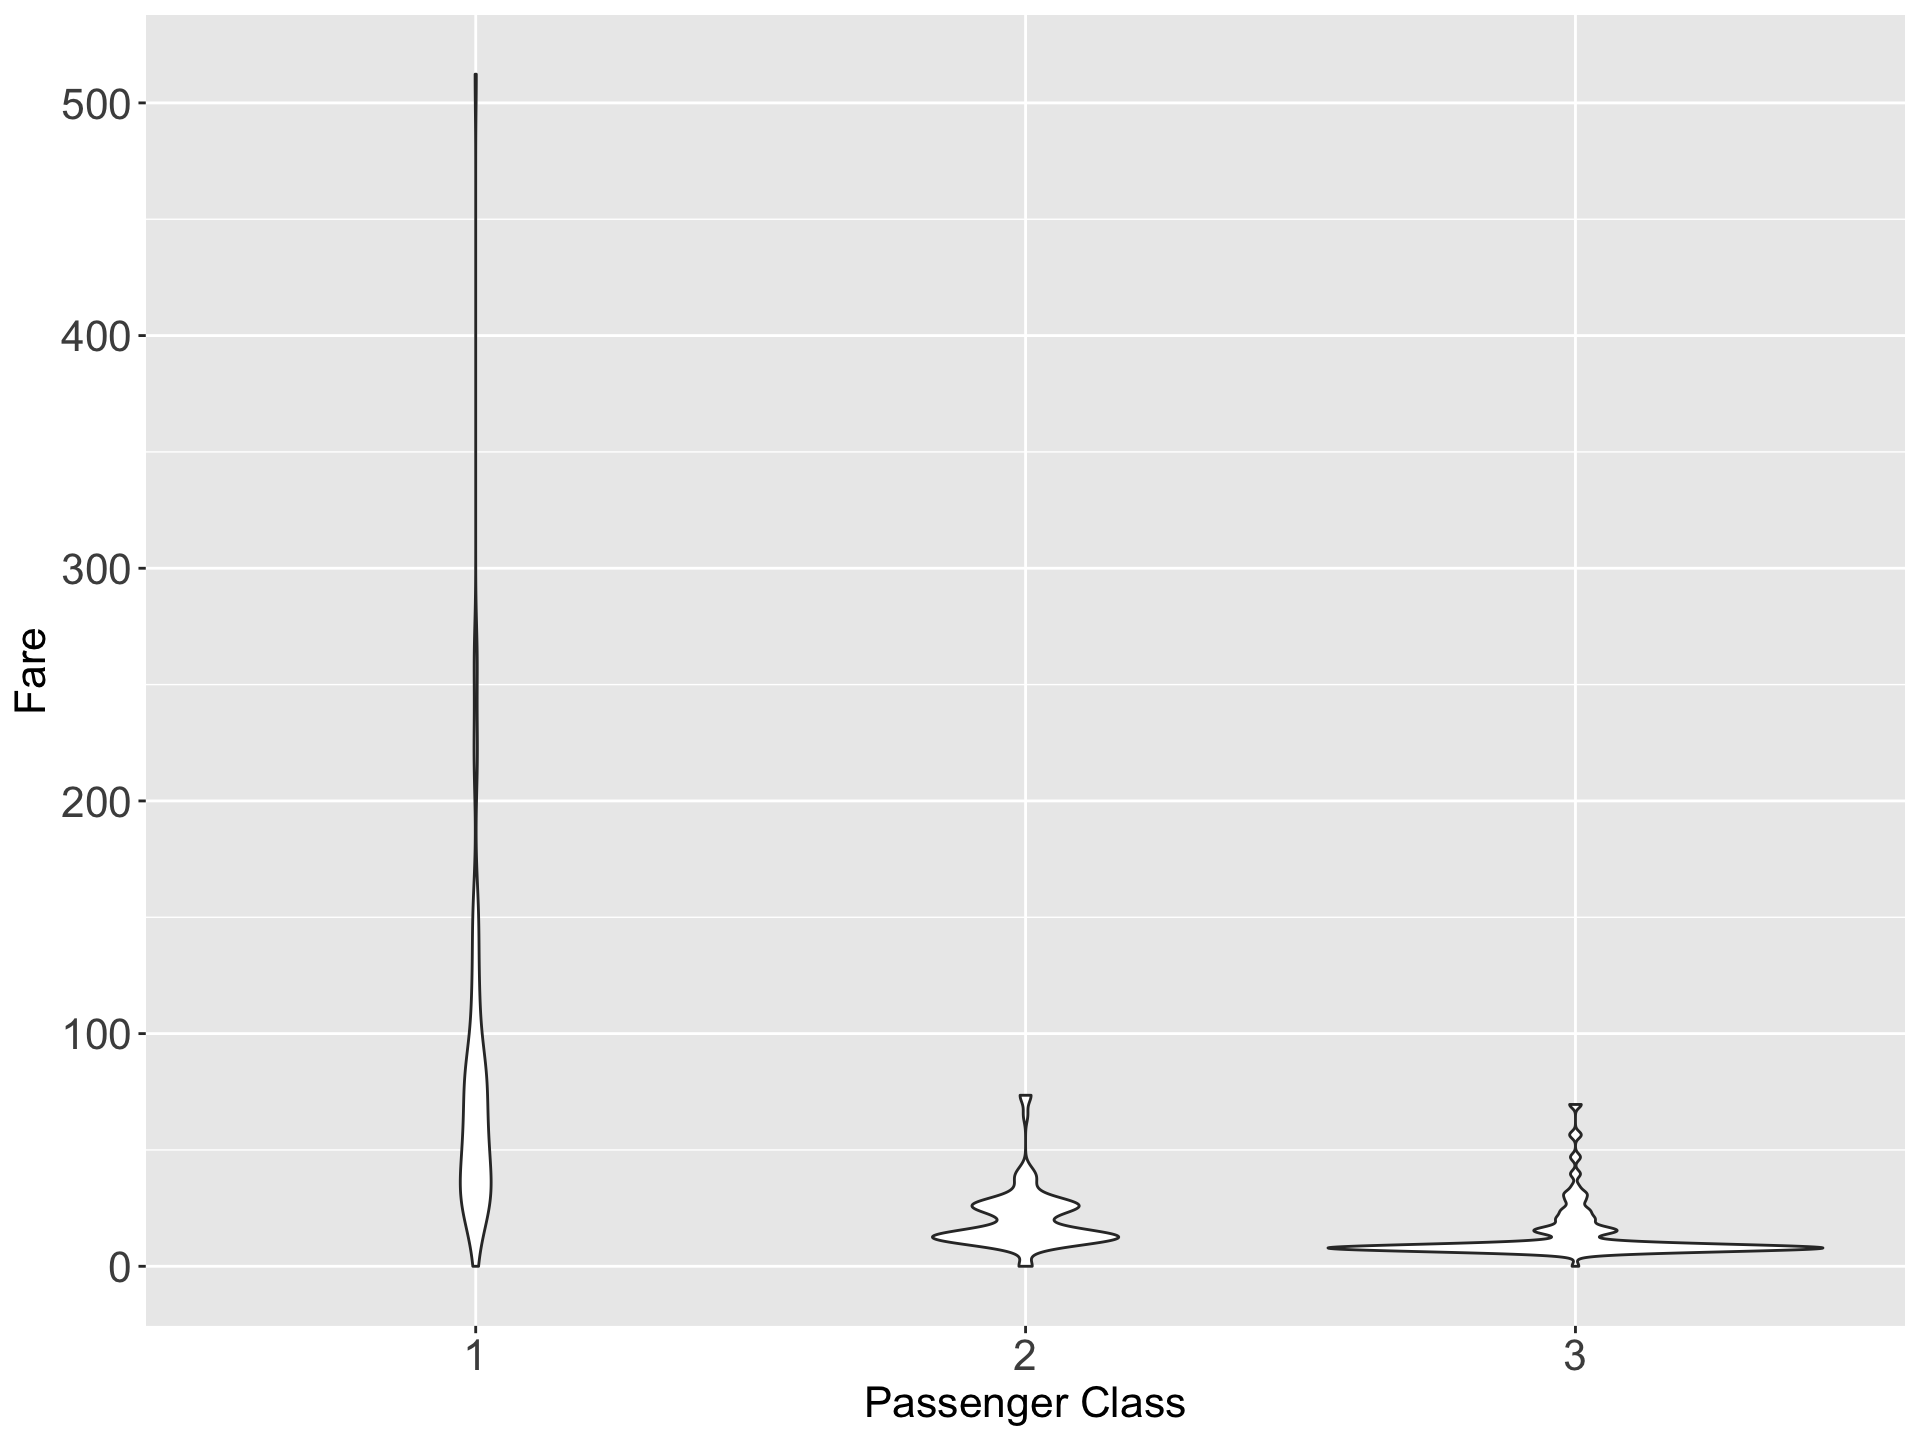
\includegraphics[width=0.8\linewidth]{figure/violin2-1} \end{center}

\newpage

\hypertarget{summary-measures}{%
\section{Summary Measures}\label{summary-measures}}

\hypertarget{measures-of-central-tendency}{%
\subsection{Measures of Central Tendency}\label{measures-of-central-tendency}}

\begin{itemize}
\item
  \textbf{Measure of central tendency} yield information about the center, or middle part, of a group of numbers.
\item
  Eg: Mode, Median, Arithmetic Mean, Geometric mean, Harmonic Mean, Quadratic Mean, Quartiles, Deciles, and Percentiles
\end{itemize}

\hypertarget{mode}{%
\subsubsection{Mode}\label{mode}}

\begin{itemize}
\item
  The Mode is the most frequently occuring value In a set of data
\item
  Organizing the data into an ordered array (an ordering of the numbers from smallest to largest) helps to locate the mode.
\item
  In the case of a tie for the most frequent occuring value, two modes are listed. Then the data are set to be \textbf{bimodal}
\item
  If a set of data is not exactly bimodal but contains two values that are more dominant than others, some researchers take the liberty of referring to the data set as bimodal even without an \emph{exact tie} for the mode.
\item
  Data sets with more than two modes are referred to as \textbf{multimodal}.
\item
  The mode is an appropriate measure of central tendency for nominal-level data.
\item
  The mode can be used to determine which category occurs most frequently.
\item
  Advantages and disadvantages of mode
\end{itemize}

\begin{center}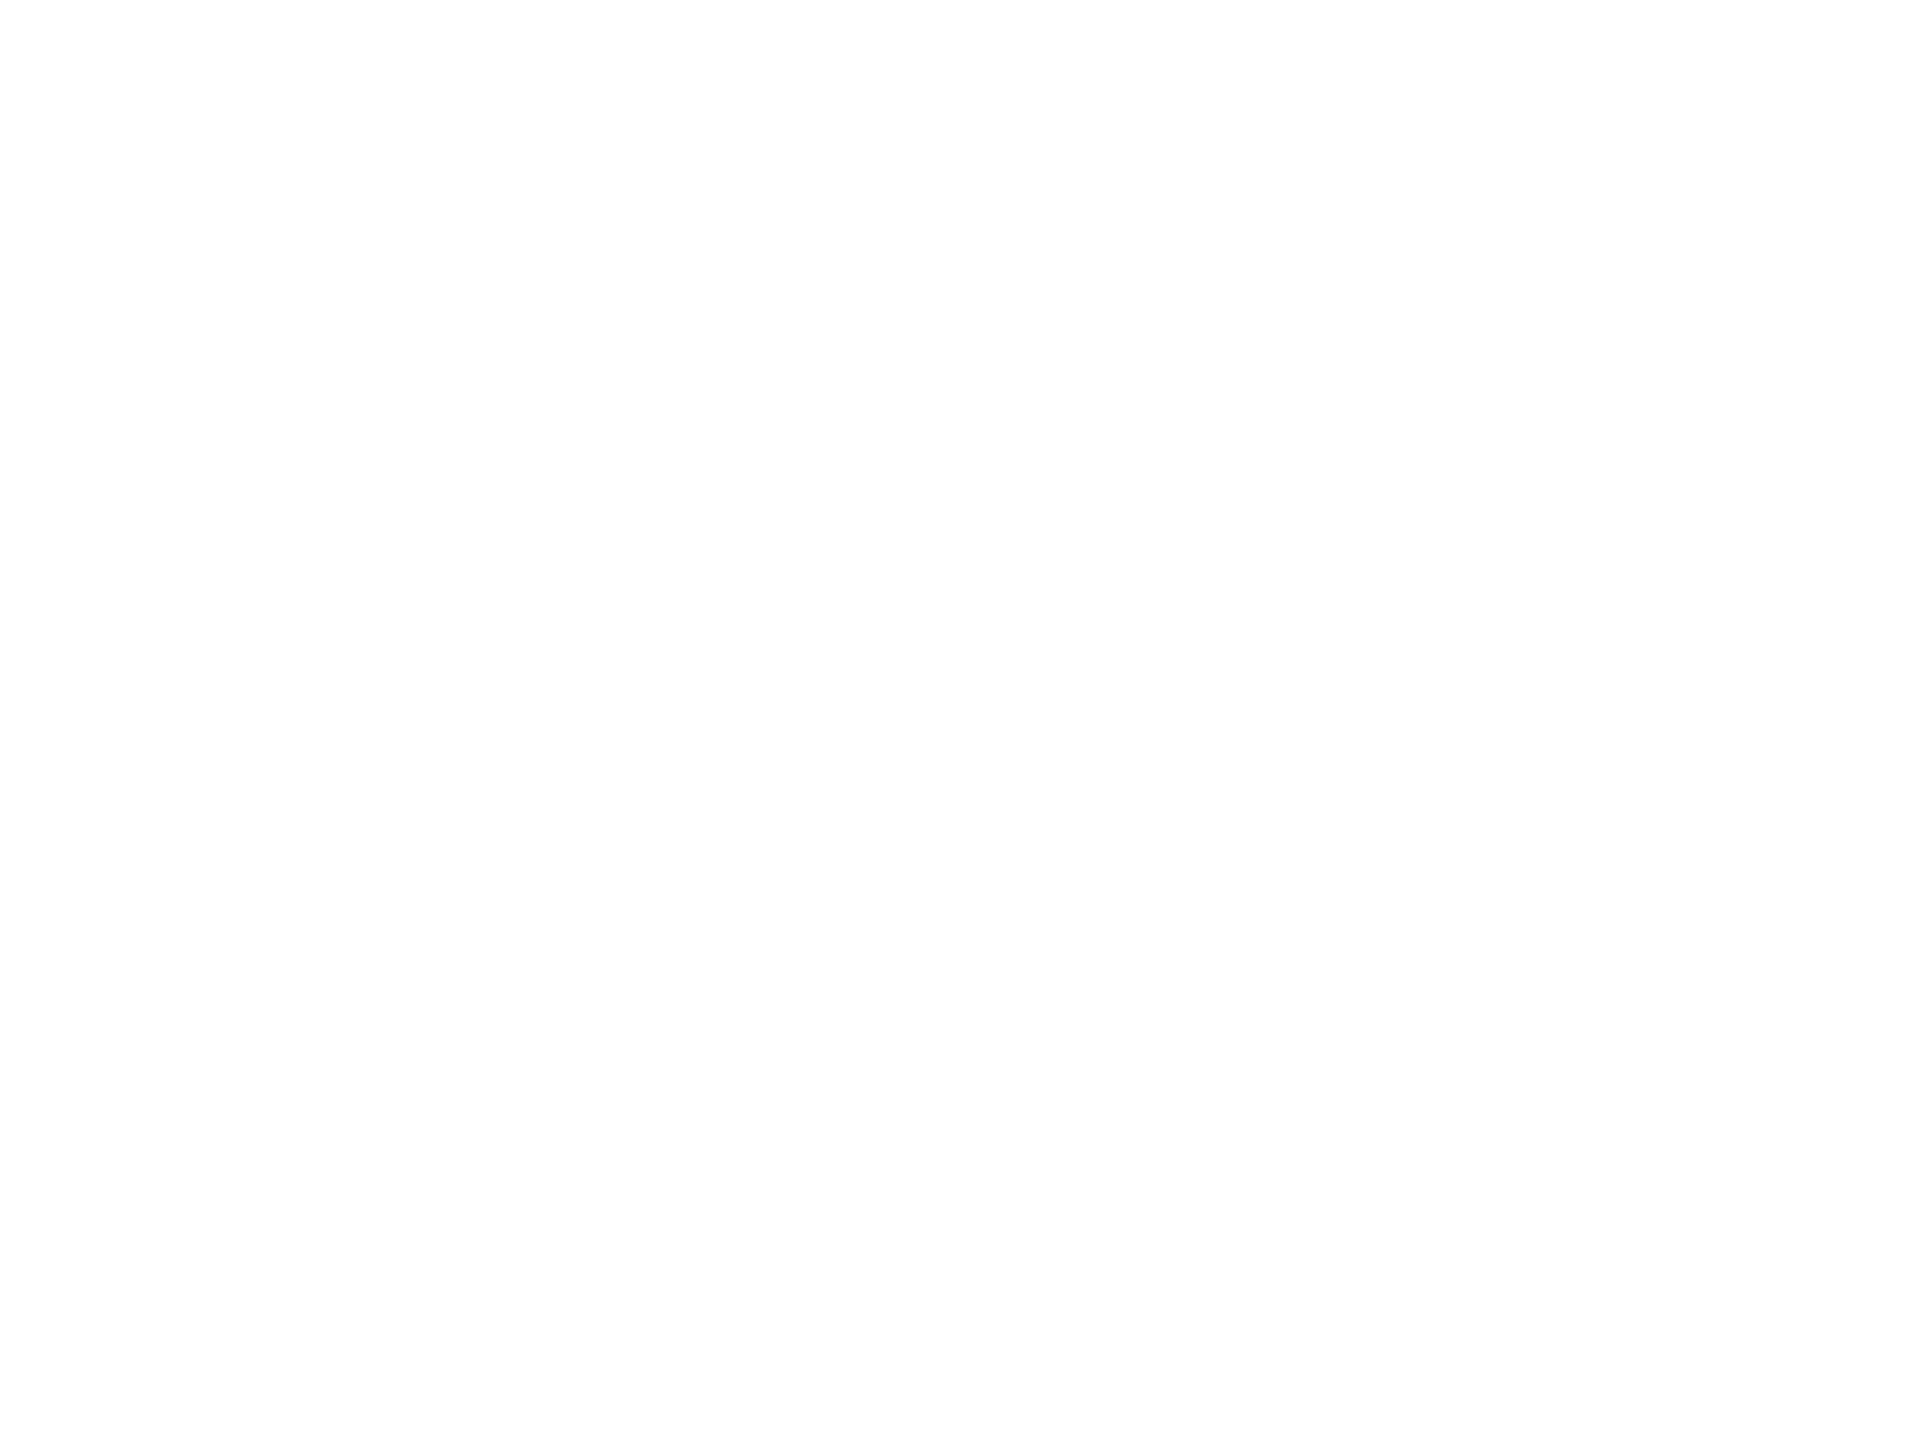
\includegraphics[width=1\linewidth]{figure/box21-1} \end{center}

\hypertarget{median}{%
\subsubsection{Median}\label{median}}

\begin{itemize}
\item
  The median is the middle value in an ordered array of numbers.
\item
  Median divides the series into equal parts
\item
  The following steps are used to determine the median.
\item
  STEP 1: Arrange the observations in an ordered data array.
\item
  STEP 2: For an \textbf{odd number} of terms, find the middle term of the ordered array. It is the median.
\item
  STEP 3: For an \textbf{even number} of terms, find the arithmetic mean of the middle two terms. This arithmetic mean is the median.
\end{itemize}

\[Median = \text{the }(\frac{n+1}{2})\text{th item in the data array} \]

\begin{itemize}
\item
  The level of data measurement must be at least ordinal for a median to be meaningful.
\item
  Advantages and disadvantages of median
\end{itemize}

\begin{center}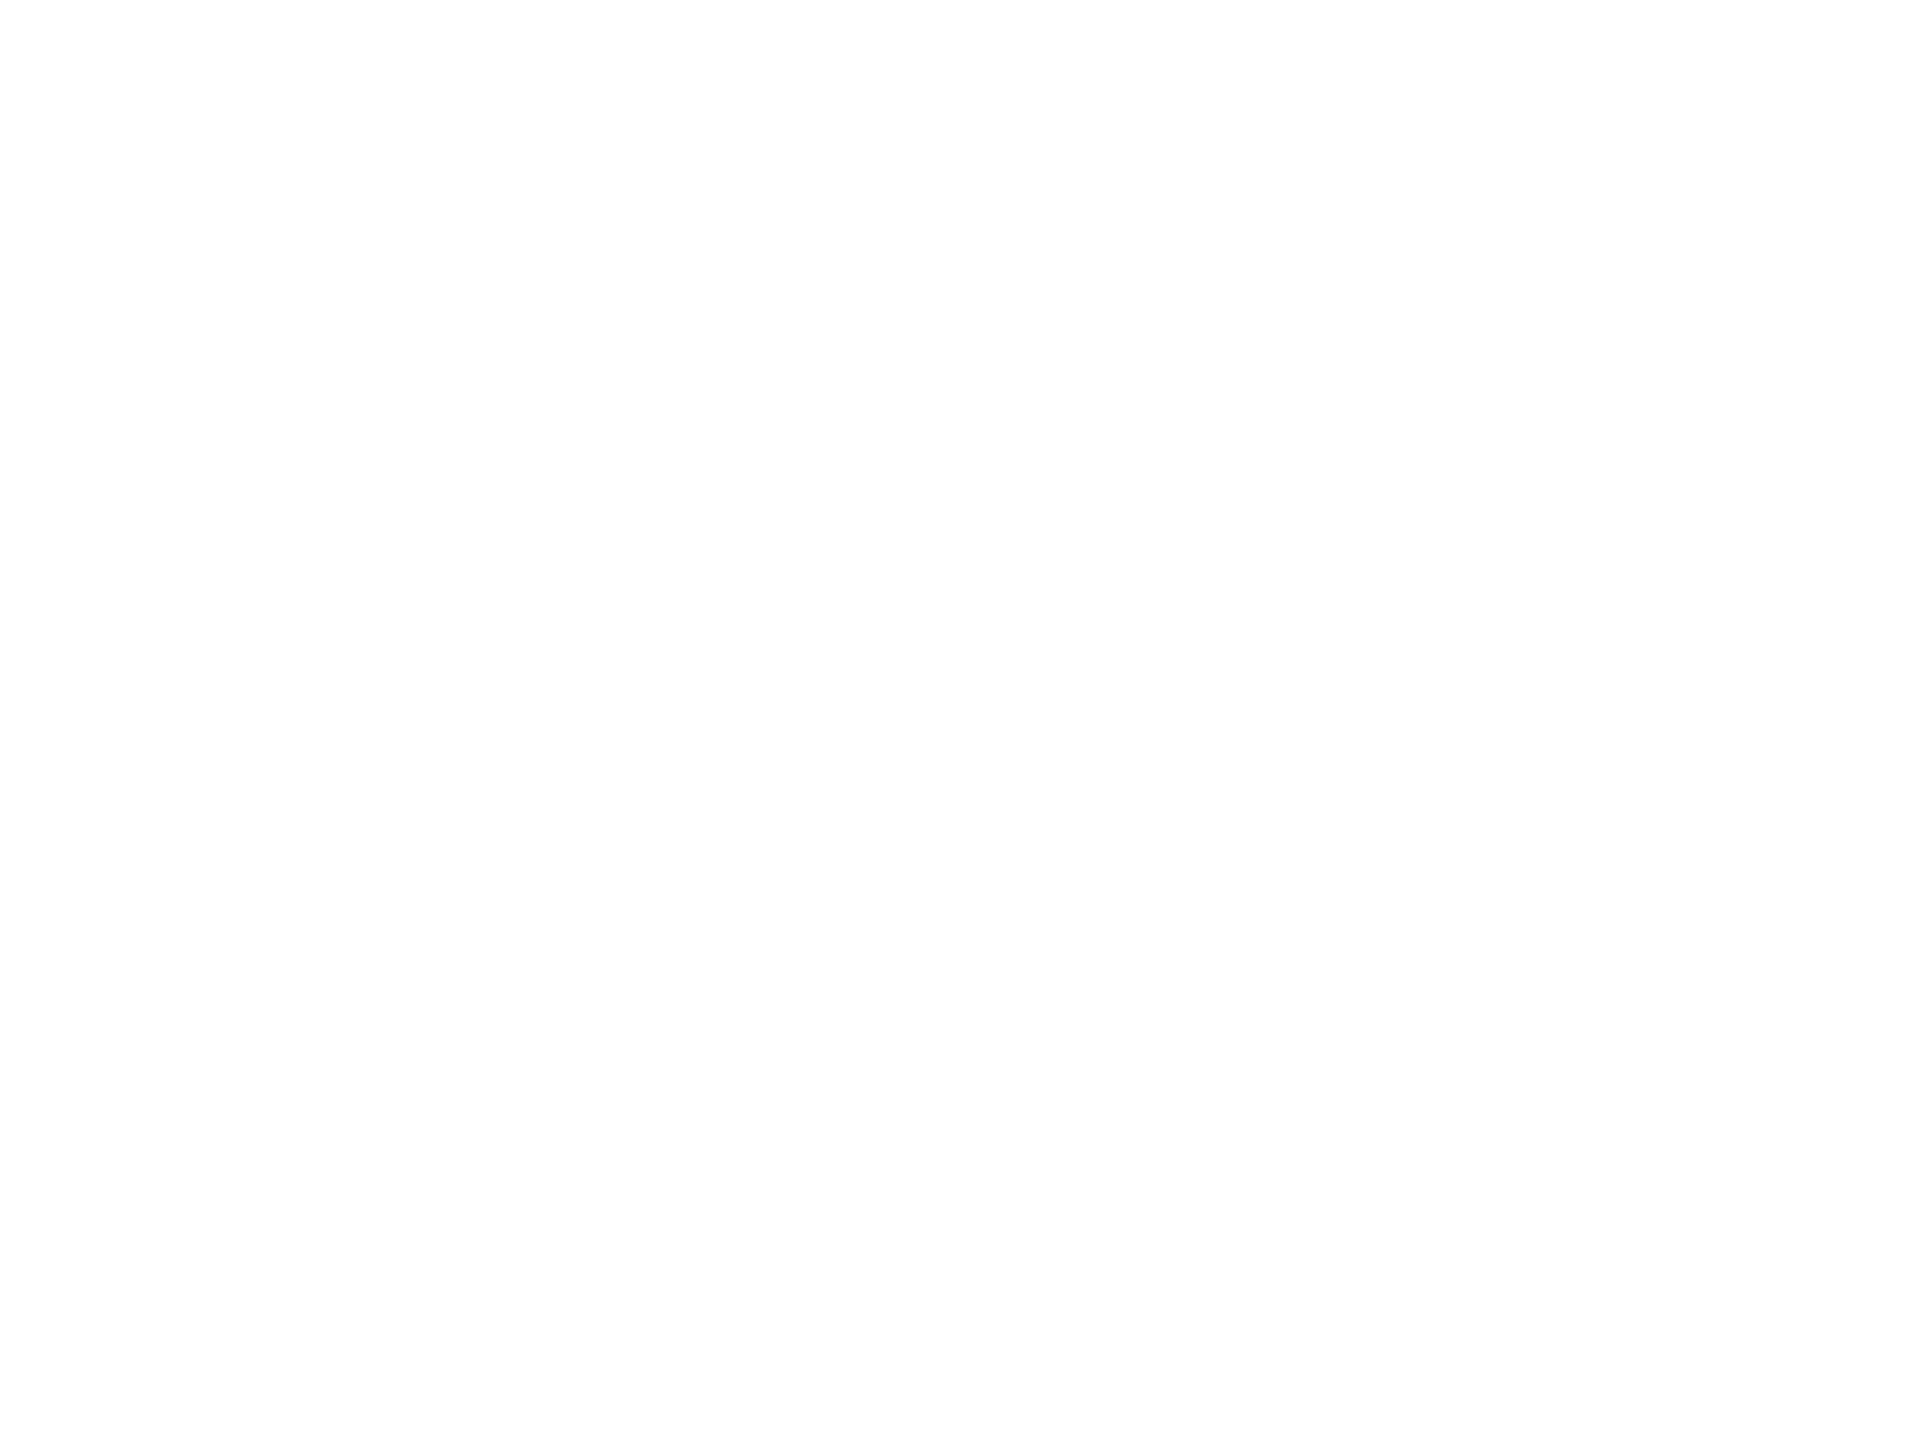
\includegraphics[width=1\linewidth]{figure/box22-1} \end{center}

\hypertarget{arithmetic-mean}{%
\subsubsection{Arithmetic Mean}\label{arithmetic-mean}}

\begin{itemize}
\item
  The arithmetic mean (usually called mean) is the sum of all observations divided by the total number of observations.
\item
  Population Mean

  \begin{itemize}
  \item
    The poupulation mean us represented by the Greek letter \(mu\) (\(\mu\)).
  \item
    Let, \(N\) is the number of terms in the population.
  \end{itemize}
\end{itemize}

\[\mu = \frac{\sum{x}}{N}=\frac{x_1+x_2+x_3+...+x_N}{N}\]

\begin{itemize}
\item
  Sample Mean

  \begin{itemize}
  \tightlist
  \item
    The sample mean is represented by \(\bar{x}\)
  \item
    Let, \(n\) is the number of terms in the sample
    \[\bar{x} = \frac{\sum{x}}{n}=\frac{x_1+x_2+x_3+...+x_n}{n}\]
  \end{itemize}
\item
  It is appropriate to use the mean to analyse data that are not at least interval level in measurement.
\item
  Advantages and disadvantages of arithmetic mean
\end{itemize}

\begin{center}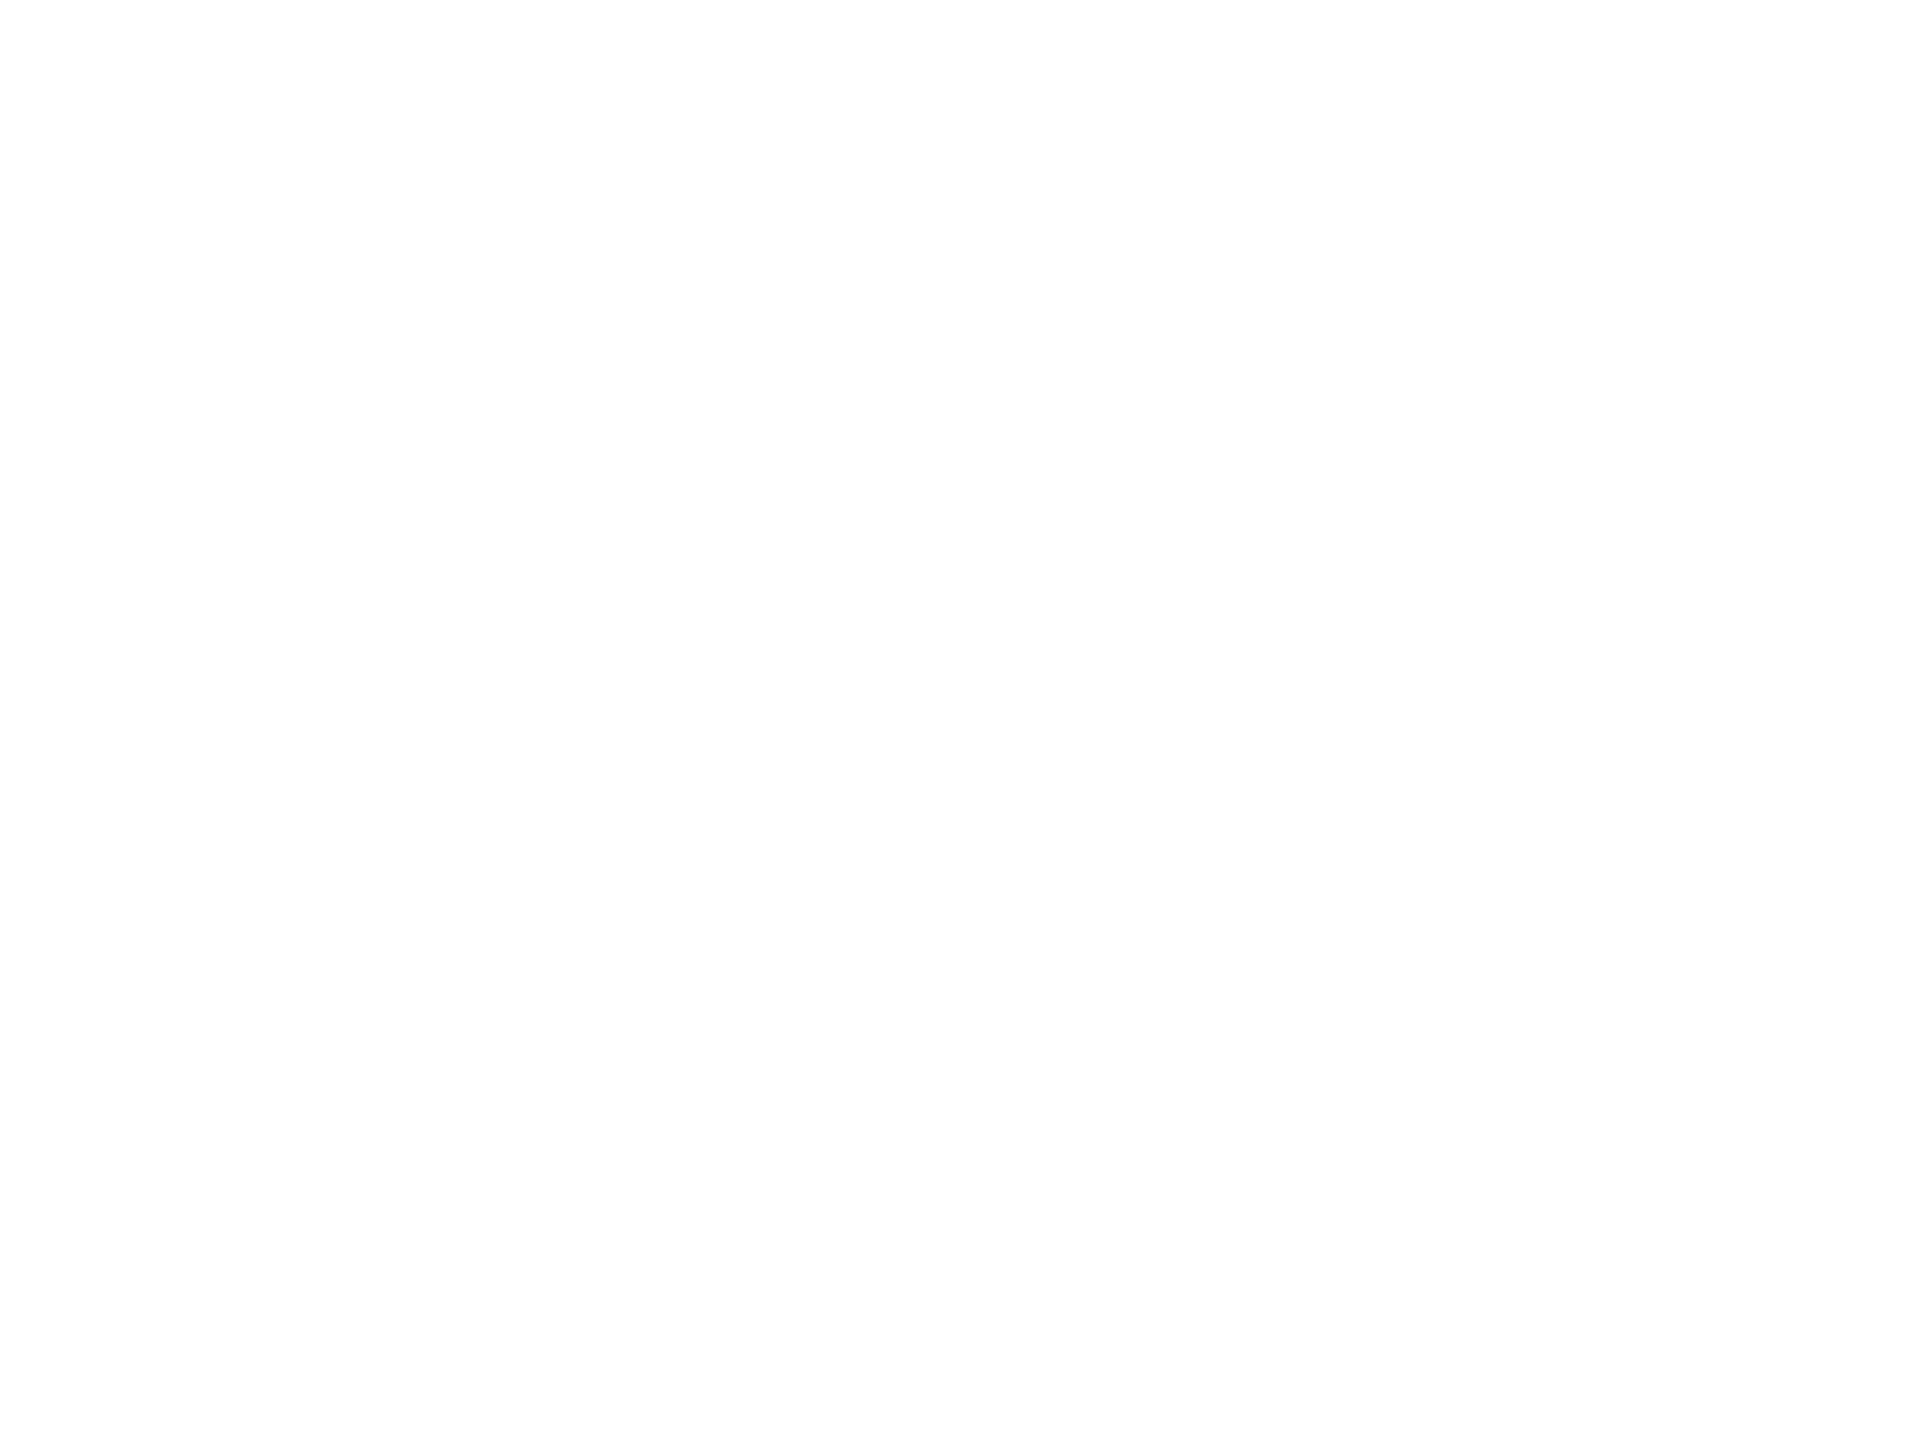
\includegraphics[width=1\linewidth]{figure/box23 -1} \end{center}

\textbf{Empirical relationship between mean, mode, median}

\begin{itemize}
\tightlist
\item
  In case of symmetrical distribution, mean, median and mode coincide \((mean = meadian= mode)\)
\end{itemize}

\begin{center}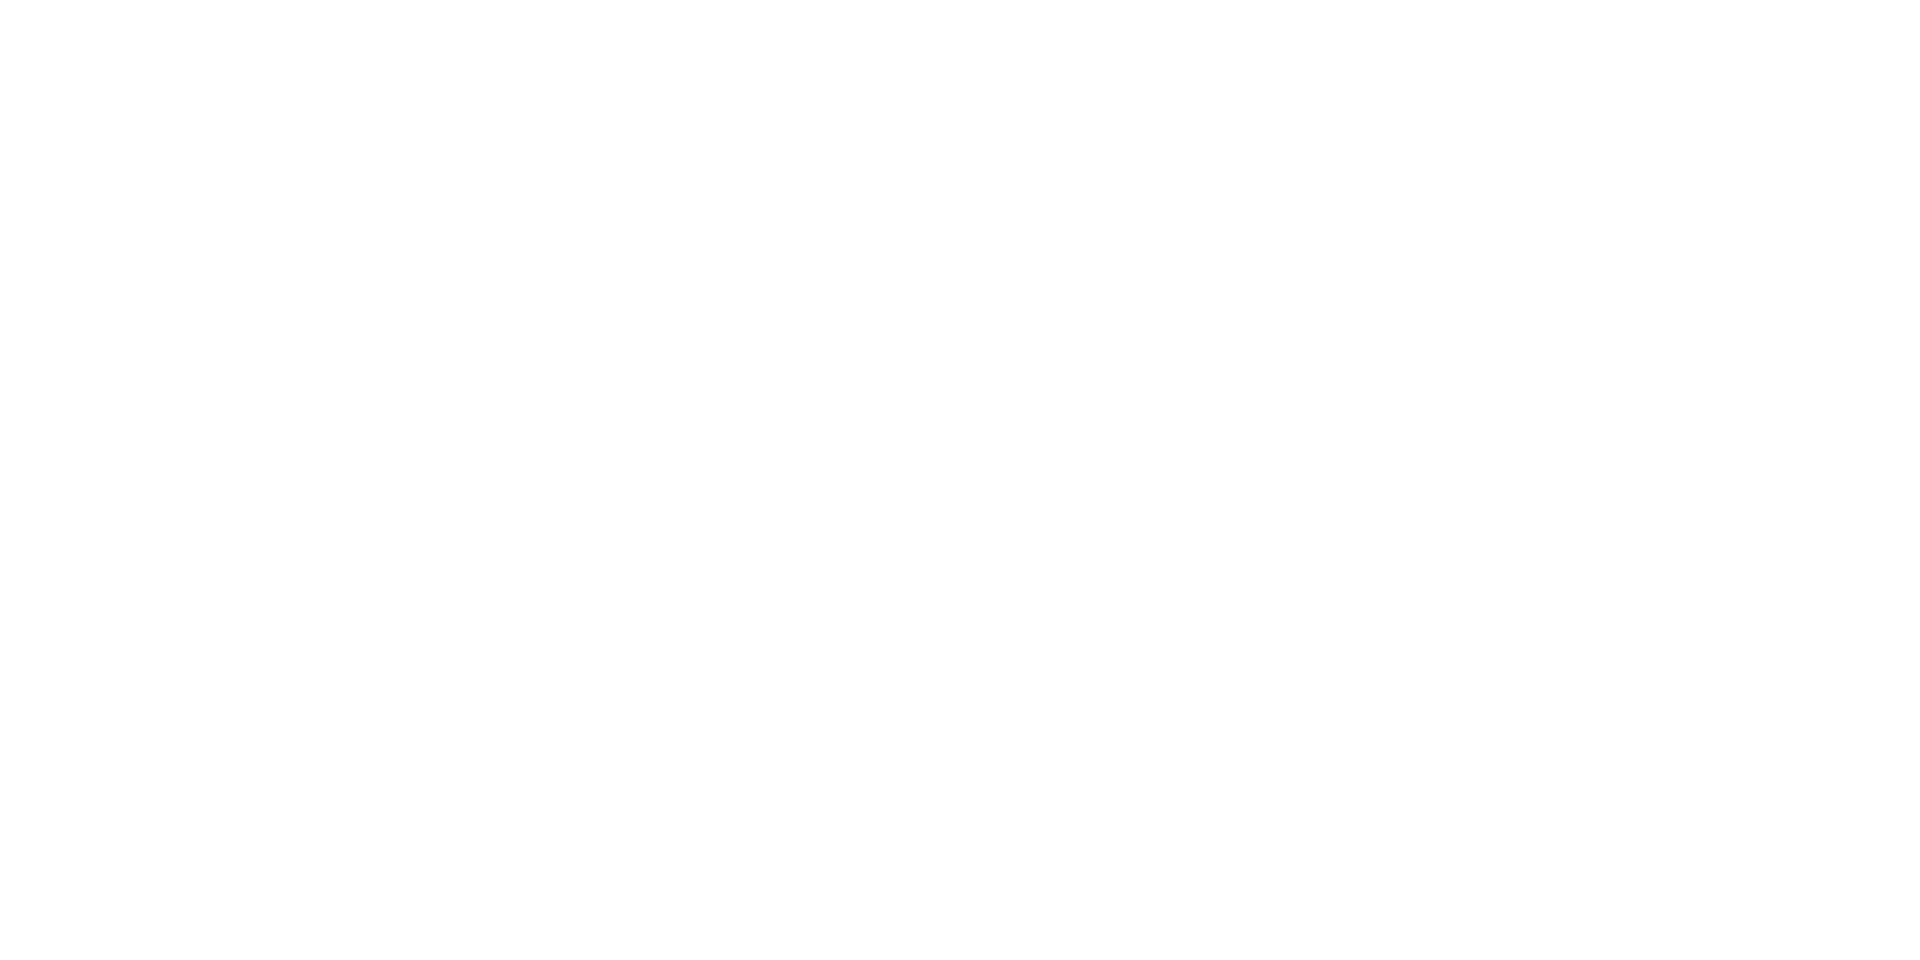
\includegraphics[width=1\linewidth]{figure/box24 -1} \end{center}

\begin{itemize}
\tightlist
\item
  For a moderately asymmetrical distribution, the following relationship exists \(Mean – Mode = 3(Mean - Median)\)
\end{itemize}

\begin{center}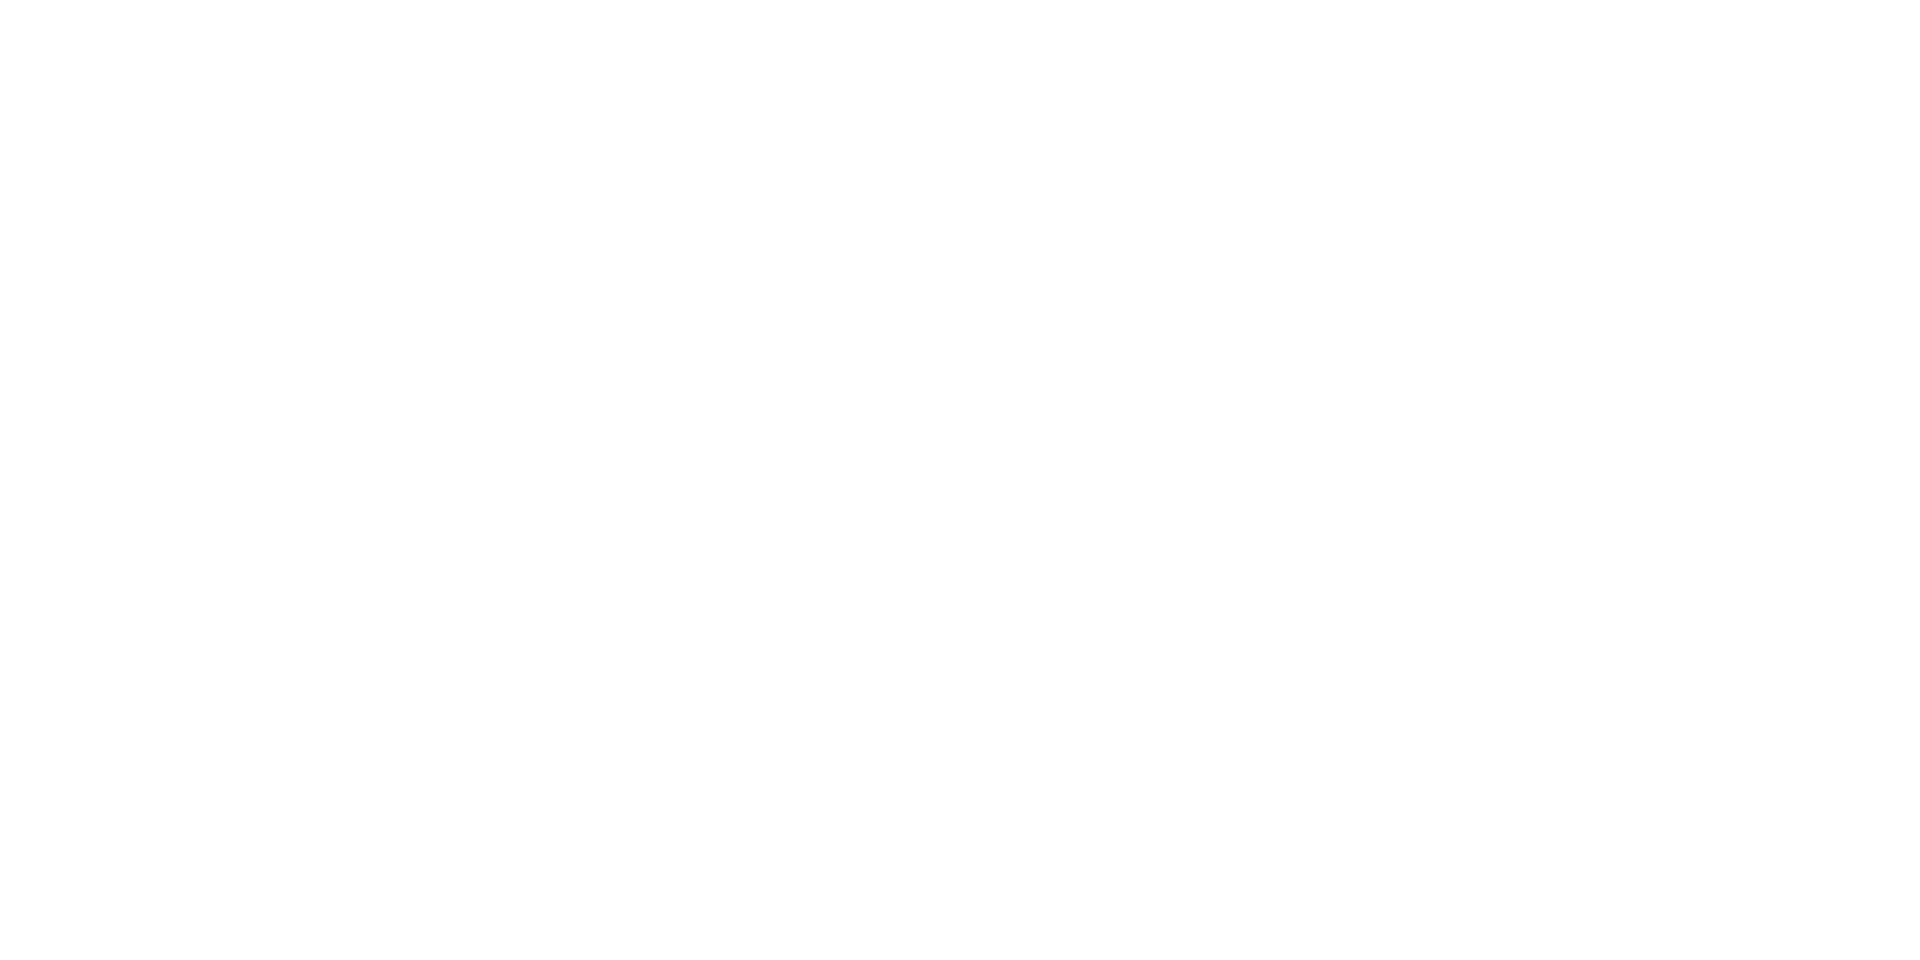
\includegraphics[width=1\linewidth]{figure/box25 -1} \end{center}

\textbf{Choice between mean and median}

\begin{itemize}
\tightlist
\item
  Mean is very sensitive to outliers.Median is not sensitive to outliers
\item
  When there are outliers in a data set, median is more appropriate than mean
\end{itemize}

\hypertarget{quartiles-deciles-and-percentiles}{%
\subsubsection{Quartiles, Deciles and Percentiles}\label{quartiles-deciles-and-percentiles}}

\begin{itemize}
\tightlist
\item
  Median divides the data set into two equal parts.
\item
  There are other values which divide the data set into a number of equal parts
\item
  Those are Quartiles, Deciles and Percentiles
\end{itemize}

\textbf{\emph{(a) Quartiles (Q) -- Quartiles divide an array into four equal parts}}

\[Q_i = \text{the }\frac{i}{4}(n+1)\text{th item in the data array} \]

\textbf{\emph{(b) Deciles (D) -- Deciles divide an array into ten equal parts}}

\[D_i = \text{the }\frac{i}{10}(n+1)\text{th item in the data array} \]

\textbf{\emph{(c) Percentiles (P) -- Percentiles divide an array into 100 equal parts}}

\[P_i = \text{the }\frac{i}{100}(n+1)\text{th item in the data array} \]

\hypertarget{measures-of-variability}{%
\subsection{Measures of Variability}\label{measures-of-variability}}

\begin{itemize}
\item
  Statistics that describe the spread or dispersion of a set of data.
\item
  Measure of central tendency yield information about particular points of a data set.
\item
  However, business researchers can use another group of analytic tools to describe a set of data.
\item
  These tools are measures of variability, which describe the spread of the dispersion of a set of data.
\item
  Using measures of variability in conjunction with measures of central tendency makes possible a more complete numerical description of the data.
\item
  This section focuses on seven measures of variability for ungrouped data: range, interquartile range, variance, standard deviation, z score and coefficient of variation.
\end{itemize}

\hypertarget{range}{%
\subsubsection{Range}\label{range}}

\begin{itemize}
\tightlist
\item
  The range is the difference between the largest value of a data set and the smallest value.
\end{itemize}

\[Range = Maximum - Minimum\]

\begin{itemize}
\item
  One important use of the range is in quality assurance, where the range is used to construct control charts
\item
  Advantages and disadvantages of range
\end{itemize}

\begin{center}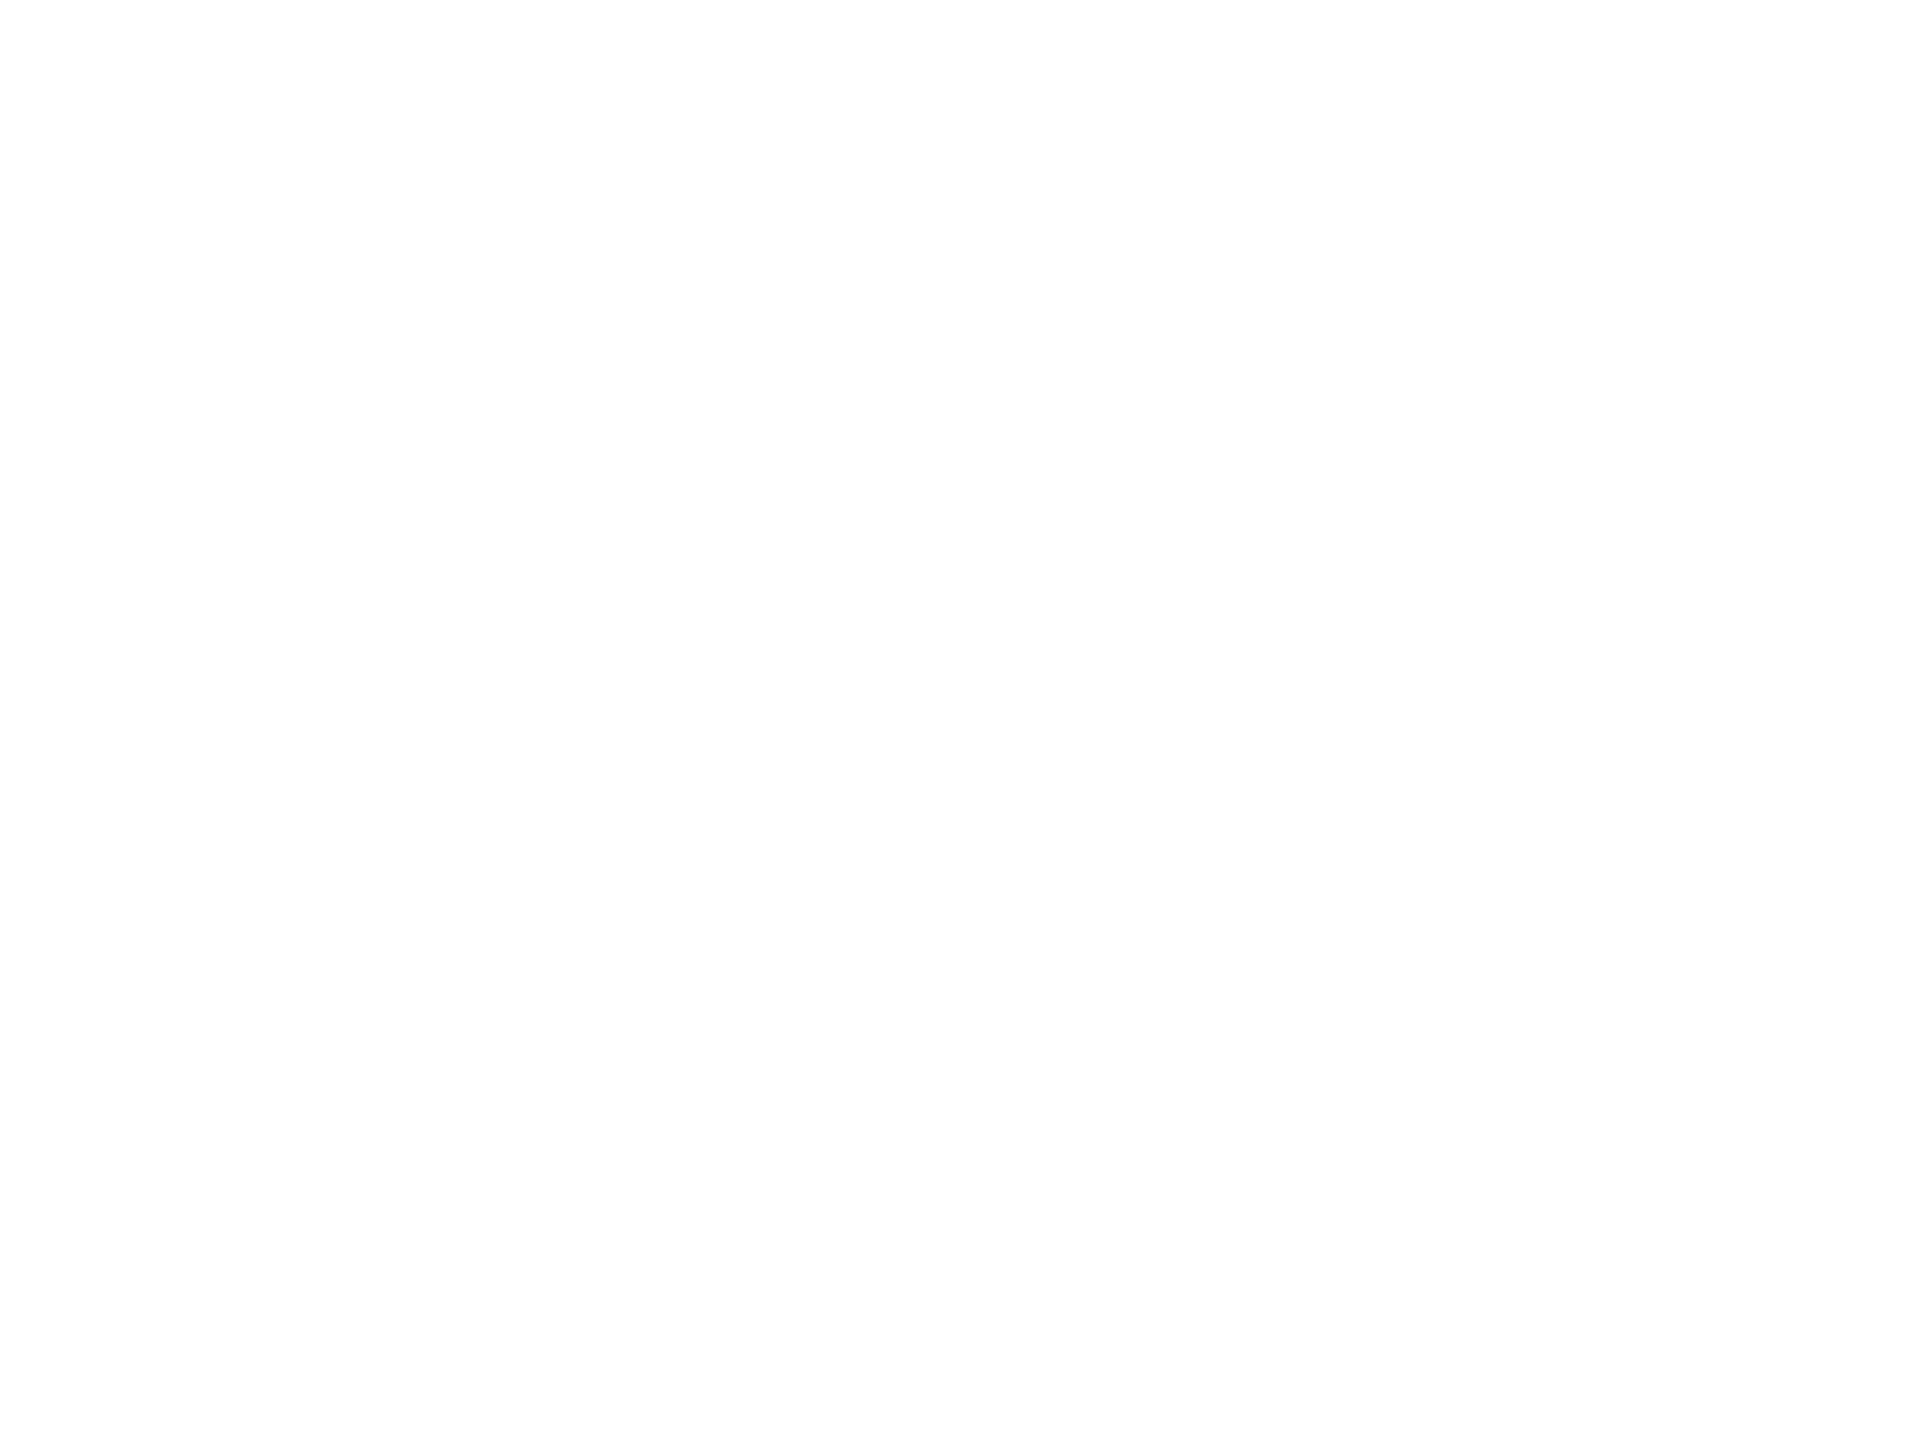
\includegraphics[width=1\linewidth]{figure/box26 -1} \end{center}

\hypertarget{interquartile-range-iqr}{%
\subsubsection{Interquartile Range (IQR)}\label{interquartile-range-iqr}}

\begin{itemize}
\item
  We use the interquartile range (IQR) to measure the spread of a data around the median (M).
\item
  The interquartile range is the range of values between the first and third quartile.
\item
  Essentially it is the range of the middle 50\% of the data and is determined by computing the value of \(Q_3 - Q_1\).
\item
  The interquartile range is especially useful in situations where data users are more interested in values towards the middle and less interested in extremes.
\item
  The interquartile range is used in the construction of box and whisker plots.
\item
  By eliminating the lowest 25\% and the highest 25\% of the items in a series, we are left with the central 50\% , which are ordinarily free of extreme values.
\end{itemize}

\begin{center}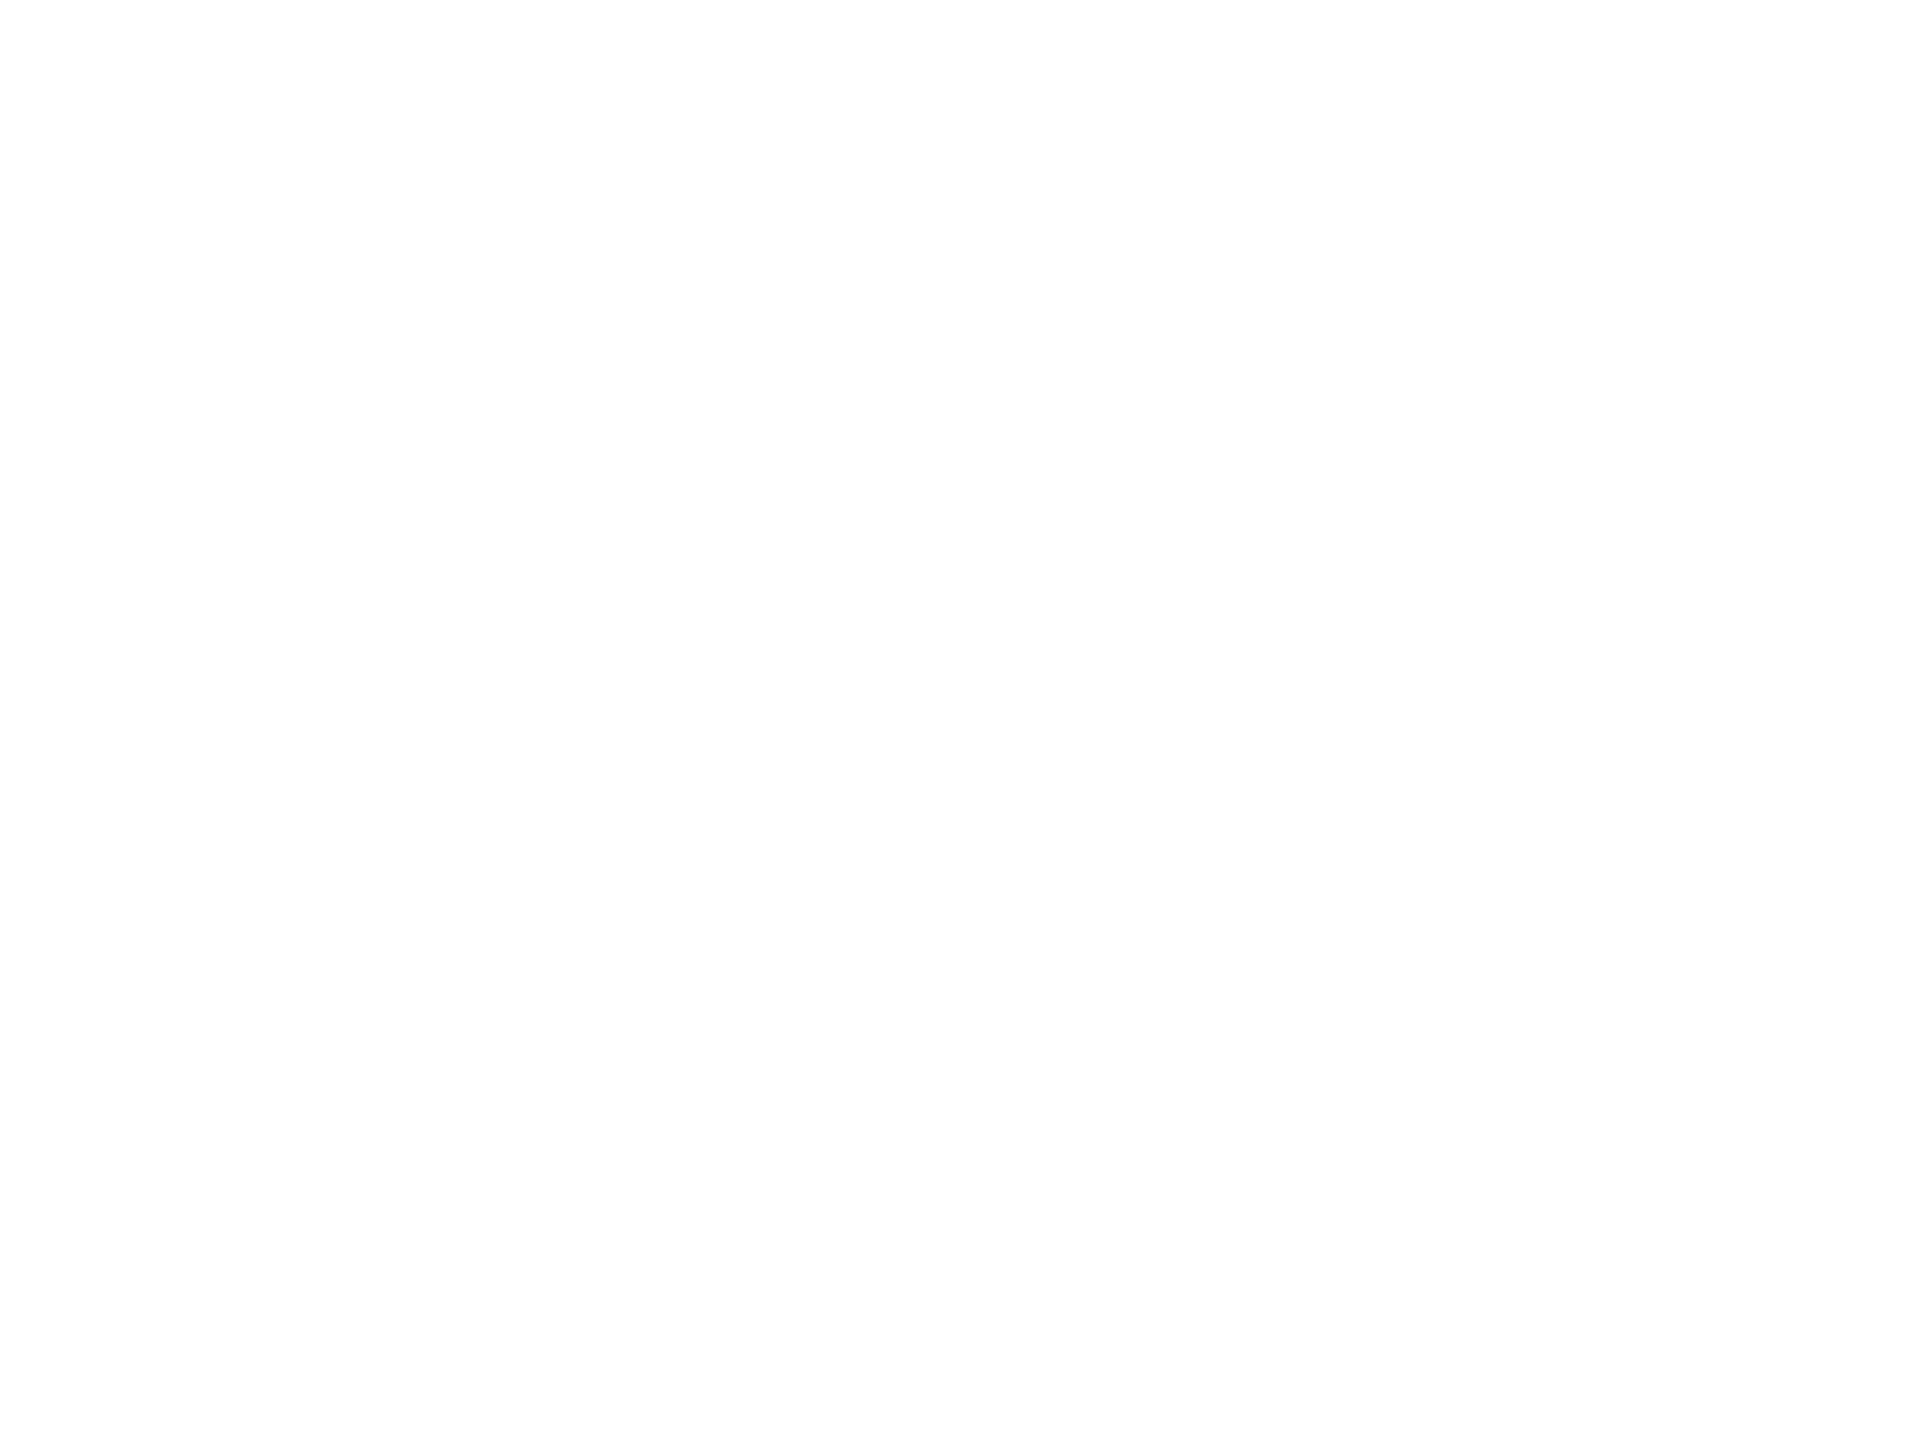
\includegraphics[width=1\linewidth]{figure/box27 -1} \end{center}

\hypertarget{variance-and-standard-deviation}{%
\subsubsection{Variance and Standard Deviation}\label{variance-and-standard-deviation}}

\hypertarget{measures-of-skewness-and-kurtosis}{%
\subsection{Measures of Skewness and Kurtosis}\label{measures-of-skewness-and-kurtosis}}

\hypertarget{measures-of-association}{%
\subsection{Measures of Association}\label{measures-of-association}}

\hypertarget{references}{%
\subsection*{References}\label{references}}
\addcontentsline{toc}{subsection}{References}

Black, K., Asafu-Adjaye, J., Khan, N., Perera, N., Edwards, P., \& Harris, M. (2007). \emph{Australasian business statistics}. John Wiley \& Sons.

\hypertarget{sets-and-relations}{%
\chapter{Sets and Relations}\label{sets-and-relations}}

\hypertarget{probability}{%
\chapter{Probability}\label{probability}}

\hypertarget{correlation-and-regression}{%
\chapter{Correlation and Regression}\label{correlation-and-regression}}

\bibliography{book.bib,packages.bib}


\end{document}
